% Options for packages loaded elsewhere
\PassOptionsToPackage{unicode}{hyperref}
\PassOptionsToPackage{hyphens}{url}
\PassOptionsToPackage{dvipsnames,svgnames,x11names}{xcolor}
%
\documentclass[
  letterpaper,
  DIV=11,
  numbers=noendperiod,
  oneside]{scrreprt}

\usepackage{amsmath,amssymb}
\usepackage{iftex}
\ifPDFTeX
  \usepackage[T1]{fontenc}
  \usepackage[utf8]{inputenc}
  \usepackage{textcomp} % provide euro and other symbols
\else % if luatex or xetex
  \usepackage{unicode-math}
  \defaultfontfeatures{Scale=MatchLowercase}
  \defaultfontfeatures[\rmfamily]{Ligatures=TeX,Scale=1}
\fi
\usepackage{lmodern}
\ifPDFTeX\else  
    % xetex/luatex font selection
\fi
% Use upquote if available, for straight quotes in verbatim environments
\IfFileExists{upquote.sty}{\usepackage{upquote}}{}
\IfFileExists{microtype.sty}{% use microtype if available
  \usepackage[]{microtype}
  \UseMicrotypeSet[protrusion]{basicmath} % disable protrusion for tt fonts
}{}
\makeatletter
\@ifundefined{KOMAClassName}{% if non-KOMA class
  \IfFileExists{parskip.sty}{%
    \usepackage{parskip}
  }{% else
    \setlength{\parindent}{0pt}
    \setlength{\parskip}{6pt plus 2pt minus 1pt}}
}{% if KOMA class
  \KOMAoptions{parskip=half}}
\makeatother
\usepackage{xcolor}
\usepackage[left=1in,marginparwidth=2.0666666666667in,textwidth=4.1333333333333in,marginparsep=0.3in]{geometry}
\usepackage{soul}
\setlength{\emergencystretch}{3em} % prevent overfull lines
\setcounter{secnumdepth}{5}
% Make \paragraph and \subparagraph free-standing
\ifx\paragraph\undefined\else
  \let\oldparagraph\paragraph
  \renewcommand{\paragraph}[1]{\oldparagraph{#1}\mbox{}}
\fi
\ifx\subparagraph\undefined\else
  \let\oldsubparagraph\subparagraph
  \renewcommand{\subparagraph}[1]{\oldsubparagraph{#1}\mbox{}}
\fi

\usepackage{color}
\usepackage{fancyvrb}
\newcommand{\VerbBar}{|}
\newcommand{\VERB}{\Verb[commandchars=\\\{\}]}
\DefineVerbatimEnvironment{Highlighting}{Verbatim}{commandchars=\\\{\}}
% Add ',fontsize=\small' for more characters per line
\usepackage{framed}
\definecolor{shadecolor}{RGB}{241,243,245}
\newenvironment{Shaded}{\begin{snugshade}}{\end{snugshade}}
\newcommand{\AlertTok}[1]{\textcolor[rgb]{0.68,0.00,0.00}{#1}}
\newcommand{\AnnotationTok}[1]{\textcolor[rgb]{0.37,0.37,0.37}{#1}}
\newcommand{\AttributeTok}[1]{\textcolor[rgb]{0.40,0.45,0.13}{#1}}
\newcommand{\BaseNTok}[1]{\textcolor[rgb]{0.68,0.00,0.00}{#1}}
\newcommand{\BuiltInTok}[1]{\textcolor[rgb]{0.00,0.23,0.31}{#1}}
\newcommand{\CharTok}[1]{\textcolor[rgb]{0.13,0.47,0.30}{#1}}
\newcommand{\CommentTok}[1]{\textcolor[rgb]{0.37,0.37,0.37}{#1}}
\newcommand{\CommentVarTok}[1]{\textcolor[rgb]{0.37,0.37,0.37}{\textit{#1}}}
\newcommand{\ConstantTok}[1]{\textcolor[rgb]{0.56,0.35,0.01}{#1}}
\newcommand{\ControlFlowTok}[1]{\textcolor[rgb]{0.00,0.23,0.31}{#1}}
\newcommand{\DataTypeTok}[1]{\textcolor[rgb]{0.68,0.00,0.00}{#1}}
\newcommand{\DecValTok}[1]{\textcolor[rgb]{0.68,0.00,0.00}{#1}}
\newcommand{\DocumentationTok}[1]{\textcolor[rgb]{0.37,0.37,0.37}{\textit{#1}}}
\newcommand{\ErrorTok}[1]{\textcolor[rgb]{0.68,0.00,0.00}{#1}}
\newcommand{\ExtensionTok}[1]{\textcolor[rgb]{0.00,0.23,0.31}{#1}}
\newcommand{\FloatTok}[1]{\textcolor[rgb]{0.68,0.00,0.00}{#1}}
\newcommand{\FunctionTok}[1]{\textcolor[rgb]{0.28,0.35,0.67}{#1}}
\newcommand{\ImportTok}[1]{\textcolor[rgb]{0.00,0.46,0.62}{#1}}
\newcommand{\InformationTok}[1]{\textcolor[rgb]{0.37,0.37,0.37}{#1}}
\newcommand{\KeywordTok}[1]{\textcolor[rgb]{0.00,0.23,0.31}{#1}}
\newcommand{\NormalTok}[1]{\textcolor[rgb]{0.00,0.23,0.31}{#1}}
\newcommand{\OperatorTok}[1]{\textcolor[rgb]{0.37,0.37,0.37}{#1}}
\newcommand{\OtherTok}[1]{\textcolor[rgb]{0.00,0.23,0.31}{#1}}
\newcommand{\PreprocessorTok}[1]{\textcolor[rgb]{0.68,0.00,0.00}{#1}}
\newcommand{\RegionMarkerTok}[1]{\textcolor[rgb]{0.00,0.23,0.31}{#1}}
\newcommand{\SpecialCharTok}[1]{\textcolor[rgb]{0.37,0.37,0.37}{#1}}
\newcommand{\SpecialStringTok}[1]{\textcolor[rgb]{0.13,0.47,0.30}{#1}}
\newcommand{\StringTok}[1]{\textcolor[rgb]{0.13,0.47,0.30}{#1}}
\newcommand{\VariableTok}[1]{\textcolor[rgb]{0.07,0.07,0.07}{#1}}
\newcommand{\VerbatimStringTok}[1]{\textcolor[rgb]{0.13,0.47,0.30}{#1}}
\newcommand{\WarningTok}[1]{\textcolor[rgb]{0.37,0.37,0.37}{\textit{#1}}}

\providecommand{\tightlist}{%
  \setlength{\itemsep}{0pt}\setlength{\parskip}{0pt}}\usepackage{longtable,booktabs,array}
\usepackage{calc} % for calculating minipage widths
% Correct order of tables after \paragraph or \subparagraph
\usepackage{etoolbox}
\makeatletter
\patchcmd\longtable{\par}{\if@noskipsec\mbox{}\fi\par}{}{}
\makeatother
% Allow footnotes in longtable head/foot
\IfFileExists{footnotehyper.sty}{\usepackage{footnotehyper}}{\usepackage{footnote}}
\makesavenoteenv{longtable}
\usepackage{graphicx}
\makeatletter
\def\maxwidth{\ifdim\Gin@nat@width>\linewidth\linewidth\else\Gin@nat@width\fi}
\def\maxheight{\ifdim\Gin@nat@height>\textheight\textheight\else\Gin@nat@height\fi}
\makeatother
% Scale images if necessary, so that they will not overflow the page
% margins by default, and it is still possible to overwrite the defaults
% using explicit options in \includegraphics[width, height, ...]{}
\setkeys{Gin}{width=\maxwidth,height=\maxheight,keepaspectratio}
% Set default figure placement to htbp
\makeatletter
\def\fps@figure{htbp}
\makeatother

\usepackage{booktabs}
\usepackage{longtable}
\usepackage{array}
\usepackage{multirow}
\usepackage{wrapfig}
\usepackage{float}
\usepackage{colortbl}
\usepackage{pdflscape}
\usepackage{tabu}
\usepackage{threeparttable}
\usepackage{threeparttablex}
\usepackage[normalem]{ulem}
\usepackage{makecell}
\usepackage{xcolor}
\KOMAoption{captions}{tableheading}
\makeatletter
\@ifpackageloaded{tcolorbox}{}{\usepackage[skins,breakable]{tcolorbox}}
\@ifpackageloaded{fontawesome5}{}{\usepackage{fontawesome5}}
\definecolor{quarto-callout-color}{HTML}{909090}
\definecolor{quarto-callout-note-color}{HTML}{0758E5}
\definecolor{quarto-callout-important-color}{HTML}{CC1914}
\definecolor{quarto-callout-warning-color}{HTML}{EB9113}
\definecolor{quarto-callout-tip-color}{HTML}{00A047}
\definecolor{quarto-callout-caution-color}{HTML}{FC5300}
\definecolor{quarto-callout-color-frame}{HTML}{acacac}
\definecolor{quarto-callout-note-color-frame}{HTML}{4582ec}
\definecolor{quarto-callout-important-color-frame}{HTML}{d9534f}
\definecolor{quarto-callout-warning-color-frame}{HTML}{f0ad4e}
\definecolor{quarto-callout-tip-color-frame}{HTML}{02b875}
\definecolor{quarto-callout-caution-color-frame}{HTML}{fd7e14}
\makeatother
\makeatletter
\makeatother
\makeatletter
\@ifpackageloaded{bookmark}{}{\usepackage{bookmark}}
\makeatother
\makeatletter
\@ifpackageloaded{caption}{}{\usepackage{caption}}
\AtBeginDocument{%
\ifdefined\contentsname
  \renewcommand*\contentsname{Table of contents}
\else
  \newcommand\contentsname{Table of contents}
\fi
\ifdefined\listfigurename
  \renewcommand*\listfigurename{List of Figures}
\else
  \newcommand\listfigurename{List of Figures}
\fi
\ifdefined\listtablename
  \renewcommand*\listtablename{List of Tables}
\else
  \newcommand\listtablename{List of Tables}
\fi
\ifdefined\figurename
  \renewcommand*\figurename{Figure}
\else
  \newcommand\figurename{Figure}
\fi
\ifdefined\tablename
  \renewcommand*\tablename{Table}
\else
  \newcommand\tablename{Table}
\fi
}
\@ifpackageloaded{float}{}{\usepackage{float}}
\floatstyle{ruled}
\@ifundefined{c@chapter}{\newfloat{codelisting}{h}{lop}}{\newfloat{codelisting}{h}{lop}[chapter]}
\floatname{codelisting}{Listing}
\newcommand*\listoflistings{\listof{codelisting}{List of Listings}}
\makeatother
\makeatletter
\@ifpackageloaded{caption}{}{\usepackage{caption}}
\@ifpackageloaded{subcaption}{}{\usepackage{subcaption}}
\makeatother
\makeatletter
\@ifpackageloaded{tcolorbox}{}{\usepackage[skins,breakable]{tcolorbox}}
\makeatother
\makeatletter
\@ifundefined{shadecolor}{\definecolor{shadecolor}{rgb}{.97, .97, .97}}
\makeatother
\makeatletter
\makeatother
\makeatletter
\@ifpackageloaded{sidenotes}{}{\usepackage{sidenotes}}
\@ifpackageloaded{marginnote}{}{\usepackage{marginnote}}
\makeatother
\makeatletter
\makeatother
\ifLuaTeX
  \usepackage{selnolig}  % disable illegal ligatures
\fi
\IfFileExists{bookmark.sty}{\usepackage{bookmark}}{\usepackage{hyperref}}
\IfFileExists{xurl.sty}{\usepackage{xurl}}{} % add URL line breaks if available
\urlstyle{same} % disable monospaced font for URLs
\hypersetup{
  pdftitle={An R Guide},
  pdfauthor={Joshua Allen},
  colorlinks=true,
  linkcolor={blue},
  filecolor={Maroon},
  citecolor={Blue},
  urlcolor={Blue},
  pdfcreator={LaTeX via pandoc}}

\title{An R Guide}
\author{Joshua Allen}
\date{2023-07-18}

\begin{document}
\maketitle
\ifdefined\Shaded\renewenvironment{Shaded}{\begin{tcolorbox}[enhanced, breakable, sharp corners, interior hidden, boxrule=0pt, borderline west={3pt}{0pt}{shadecolor}, frame hidden]}{\end{tcolorbox}}\fi

\renewcommand*\contentsname{Table of contents}
{
\hypersetup{linkcolor=}
\setcounter{tocdepth}{2}
\tableofcontents
}
\bookmarksetup{startatroot}

\hypertarget{who-is-this-for}{%
\chapter*{Who is This For?}\label{who-is-this-for}}
\addcontentsline{toc}{chapter}{Who is This For?}

\markboth{Who is This For?}{Who is This For?}

This guide was initially compiled for my Introduction to Political
Science Research class however this book is really for anybody who is
looking to get started in R and R Studio. The guide itself was to put it
mildly a little chaotic and somewhat difficult to navigate. So this is
my attempt to correct that. The goal of this guide is to provide a
summary of the things that helped me and add some of my own flare. By no
means is this meant to be a definitive guide to \texttt{R}. Hopefully it
is just a gentle guide and a potential reminder of things you already
know, or an introduction to things you did not know that R could do.

This ``book'' requires a significant amount of attribution to a ton of
people. In particular Much of the content is based on
\url{https://github.com/uo-ec607/lectures} by Dr.~Grant McDermott,
\url{https://talks.andrewheiss.com/2021-seacen/01-tidyverse.html} by
Dr.~Andrew Heiss as well as just general knowledge dispensed from
\href{https://www.andrewheiss.com/blog/}{his blog} and peppering him
with questions, and
\href{https://rstudio-conf-2022.github.io/ggplot2-graphic-design/}{Graphic
Design with ggplot2} by Dr.~Cédric Scherer. I highly recommend that you
check out these sources! As it stands right now I need to go back
through and add attribution to the individual chapters. Most of this
``book'' is me just translating \texttt{R} into how I think and what
helped me learn \texttt{R}.

\bookmarksetup{startatroot}

\hypertarget{pep-talk}{%
\chapter*{Pep talk}\label{pep-talk}}
\addcontentsline{toc}{chapter}{Pep talk}

\markboth{Pep talk}{Pep talk}

\begin{tcolorbox}[enhanced jigsaw, breakable, opacitybacktitle=0.6, colframe=quarto-callout-important-color-frame, bottomrule=.15mm, opacityback=0, toprule=.15mm, coltitle=black, toptitle=1mm, colback=white, titlerule=0mm, bottomtitle=1mm, colbacktitle=quarto-callout-important-color!10!white, title=\textcolor{quarto-callout-important-color}{\faExclamation}\hspace{0.5em}{Important}, rightrule=.15mm, arc=.35mm, leftrule=.75mm, left=2mm]

``There is no way of knowing nothing about a subject to knowing
something about a subject without going through a period of much
frustration and suckiness\ldots{} Push through. You'll suck less''

\begin{itemize}
\tightlist
\item
  Hadley Wickham, author of ggplot2
\end{itemize}

\end{tcolorbox}

I sucked at this initially. We all sucked at this initially. You will
often miss a comma somewhere, and your code will not run. You will be
puzzled why something is not working and get frustrated and not know why
your code is running and why somebody else's code is running to find out
later you misspelled something. I generated a ton of errors just
compiling this guide. You eventually get better at figuring out the
likely culprits and more carefully looking at your code. This is just
something that comes with practice.


\includegraphics[width=5.89in,height=\textheight]{figs/learning-r.png}

It is 100\% okay to Google stuff when working on your analysis, problem
sets, . We all do it! If I run into an issue, I do not know how to fix I
immediately google it. Remember, the goal of this class is to teach you
how to do research \texttt{R} is a minor part in the grand scheme of
things when you are doing research. My goal is to teach you how to
conduct research, not to make you a computer scientist or \texttt{R}
developer.

:::

\part{Installation and Basics}

\bookmarksetup{startatroot}

\hypertarget{before-we-get-to-the-fun-stuff}{%
\chapter{Before We Get to The Fun
Stuff}\label{before-we-get-to-the-fun-stuff}}

One of the things that I have found is unintuitive for a lot of people
when they are first learning \texttt{R} is how a computer thinks. A
computer is very good at doing stuff quickly, but needs proper
instructions. For things like an excel spreadsheet you can just open it
and do things like \texttt{=Average(C2)} and it will just work. For Word
you can just like drag and drop things without ever having to think
about how the computer knows where an image is. \texttt{R} and other
programming languages require some thought about things like this. So
this chapter will introduce you to some of these things.

\hypertarget{working-directories}{%
\section{Working Directories}\label{working-directories}}

What is a working directory? Working directories are essentially the
internal gps of the computer. You know(generally) where the stuff on
your computer is you navigate by clicking on stuff and voila you found
your stuff. Underneath the hood your computer is finding stuff by
navigating along the working directory. On my computer to get to this R
guide I click on my teaching folder, then I click on the Administrative
Stuff folder, and then I click on the \texttt{R-guide.qmd} or
\texttt{R-guide.html} file. This is what that process looks like for the
computer

\begin{Shaded}
\begin{Highlighting}[]
\FunctionTok{getwd}\NormalTok{() }\CommentTok{\# this is the working directory for the r guide}
\end{Highlighting}
\end{Shaded}

\begin{verbatim}
[1] "/Users/josh/Library/CloudStorage/Dropbox/pols-3800"
\end{verbatim}

Each \texttt{/} is essentially a click until you get to the final
destination.

Heuristically you can think of it like this.

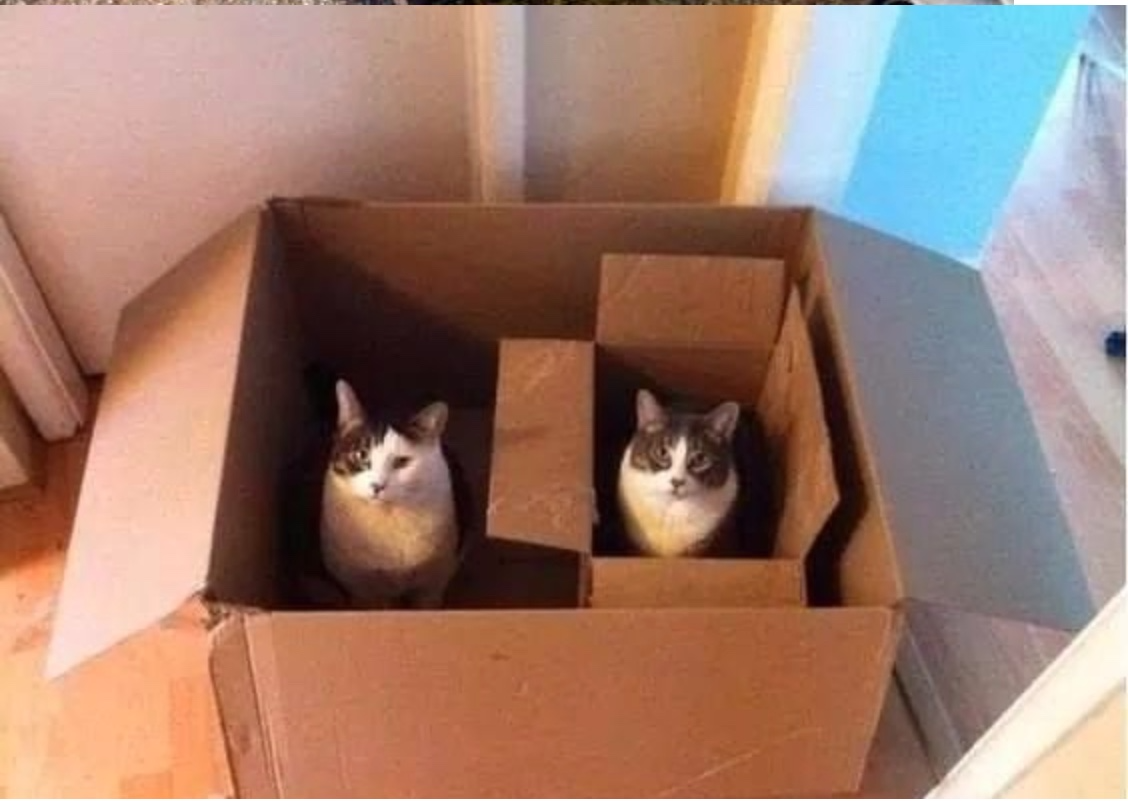
\includegraphics[width=3.76in,height=\textheight]{figs/cats-boxes.png}

\begin{itemize}
\tightlist
\item
  You \textbf{can} put a box inside a box.

  \begin{itemize}
  \tightlist
  \item
    This means folders can contain other folders.
  \item
    When you put a folder inside another folder this is called creating
    a subdirectory
  \end{itemize}
\item
  You \textbf{can} put a cat inside a box

  \begin{itemize}
  \tightlist
  \item
    This means you can put a file inside a folder.
  \end{itemize}
\item
  You \textbf{can} put a cat inside a box inside of a box

  \begin{itemize}
  \tightlist
  \item
    This means you can put a file inside a folder inside another folder
  \end{itemize}
\item
  You \textbf{cannot} put a box inside a cat

  \begin{itemize}
  \tightlist
  \item
    You cannot put a folder inside a document(thats not how computers
    work)
  \end{itemize}
\item
  You \textbf{cannot} put cat in a cat

  \begin{itemize}
  \tightlist
  \item
    This means you cannot put files inside other files. Admittedly this
    is where the metaphor breaks down.
  \end{itemize}
\end{itemize}

So to include the cat pictures in this guide, I stored it in a folder
called \texttt{figs} so to tell \texttt{R} to navigate to the picture, I
do something like this.

\begin{verbatim}
# how you navigate to folders on mac
![](figs/cats-boxes.png) # this one way to include pics in a markdown doc
\end{verbatim}

The \texttt{/} is you telling the computer that within the figs folder,
there is a file I want you to include named \texttt{cats-boxes.png}.
Windows does this slightly differently by doing something like

\begin{verbatim}
![](figs\cats-boxes.png)
\end{verbatim}

To manually set your working directory you do this

\begin{Shaded}
\begin{Highlighting}[]
\FunctionTok{setwd}\NormalTok{(}\StringTok{"path/to/your/files"}\NormalTok{) }\CommentTok{\# mac and linux}
\FunctionTok{setwd}\NormalTok{(}\StringTok{"path}\SpecialCharTok{\textbackslash{}t}\StringTok{o\textbackslash{}your}\SpecialCharTok{\textbackslash{}f}\StringTok{iles"}\NormalTok{) }\CommentTok{\# windows}
\end{Highlighting}
\end{Shaded}

\hypertarget{working-in-projects}{%
\section{Working in Projects}\label{working-in-projects}}

However, working in R projects is best practice for various reasons. A
projected-oriented workflow starts you off with a clean slate, so
problem set 0 stuff is not still loaded. It also prevents you from
constantly having to set the working directory.

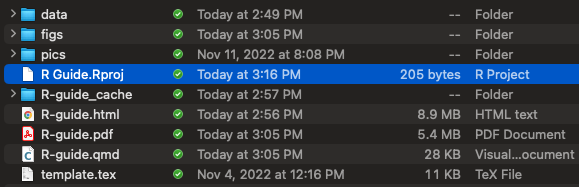
\includegraphics[width=1.93in,height=\textheight]{figs/r-project-in-folder.png}

When you start working on a problem set click on the \texttt{.Rproj}
file. This will open up RStudio, and you should be ready to go!

To open a new project open R-Studio. In the top left you will see
something that looks like a blank page. If you look to the right there
is an R with a \texttt{+} and like a weirdish blue background. Click on
that and you should see a menu that looks like.

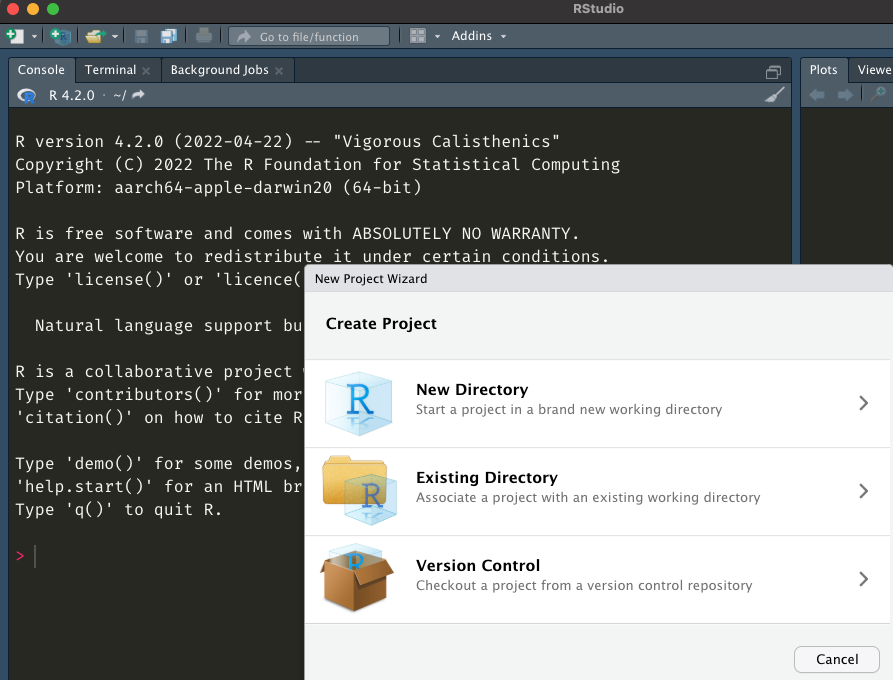
\includegraphics{figs/r-projects-menu.png}

For your final projects you are going to want to click new directory,
then click new project. You should be looking at a menu that looks like
this

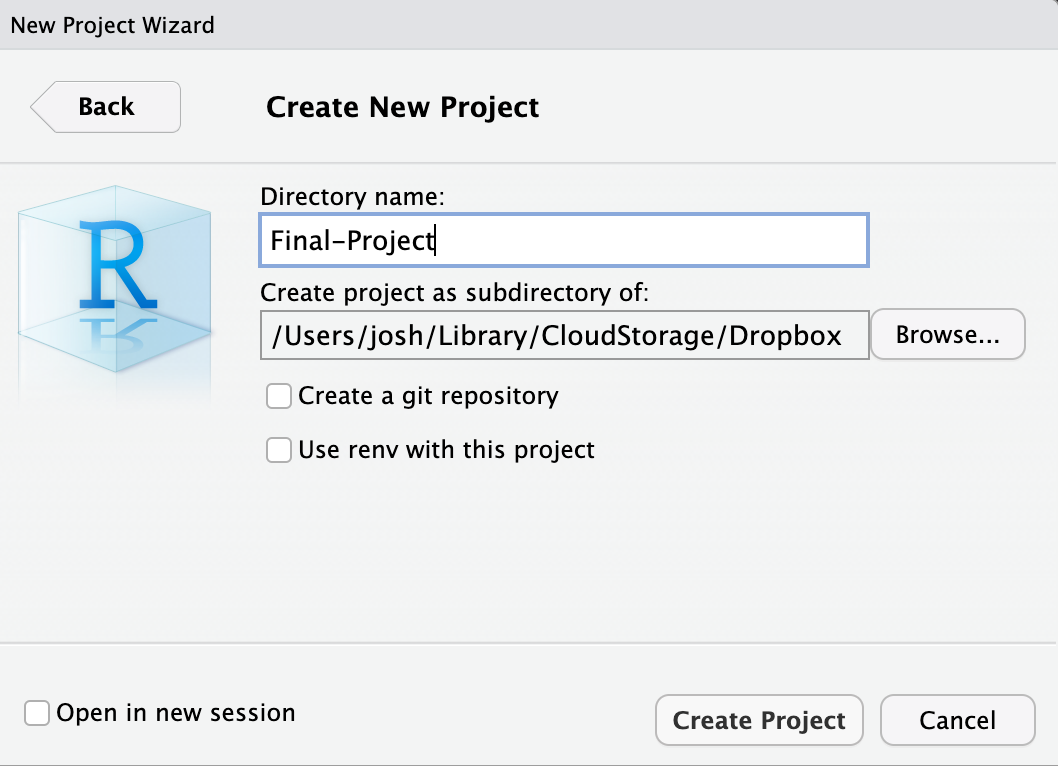
\includegraphics{figs/projects-directory-name.png}

In the directory name portion put in an informative name like
\texttt{Final-Project} or \texttt{ggplot\ lab}. If you look at the
bottom of the box you will notice that it will place the folder in my
Dropbox folder. If you click on browse you can can change where the
folder is put on your computer.

\textbf{I strongly recommend you create a dedicated folder for your
porjects instead of keeping everything on your desktop or downloads
folder}

\hypertarget{zip-files}{%
\section{Zip Files}\label{zip-files}}

To keep everything together in the same working directory I distribute
the problem sets as Zip files. You will likely encounter these at some
point in your professional life. If you want to send a folder via email
to your boss or your direct reports that has lots of stuff like images
than the chances are that you will have to send a Zip file because
Outlook has a max file size of 33mb which is next to nothing. So it is
worth spending a little time on how to unzip a file.

\hypertarget{mac}{%
\subsection{Mac}\label{mac}}

Fortunately for Mac users this is really easy. When you click download
you will see something that looks like this

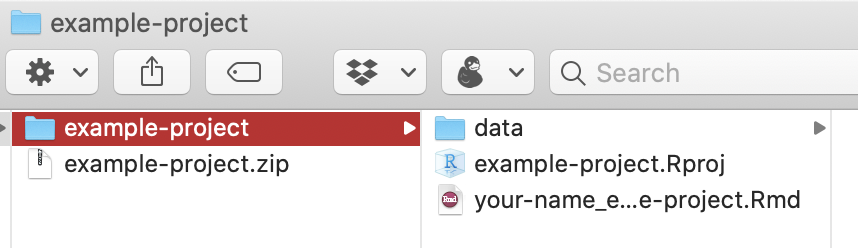
\includegraphics{pics/unzip-mac.png}

Double click on the downloaded .zip file. macOS will automatically
create a new folder with the same name as the .zip file, and all the
file's contents will be inside. Double click on the RStudio Project file
(.Rproj) to get started.

\hypertarget{windows}{%
\subsection{Windows}\label{windows}}

For Windows users this process is a bit more involved for reasons that
are unclear to me. This can be at best an inconvenience at worst it can
result in you doing all your work trying to save it and it disappearing
into the abyss. One of the things that makes this incredibly confusing
is that when you download the zip file it looks like a regular folder.

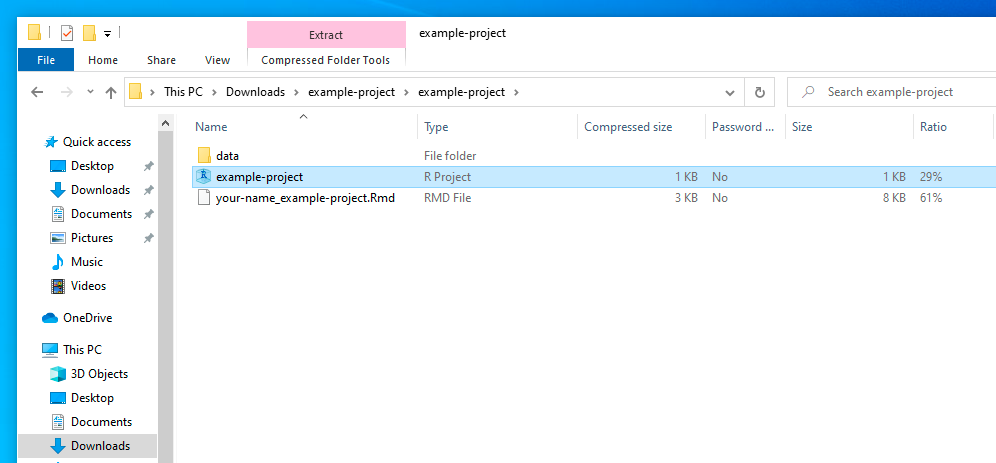
\includegraphics{pics/inside-zip-windows.png}

You can click around in it and even edit files within the zip file!
Here's what it looks like---the only clues that this folder is really a
\texttt{.zip} file are that there's a ``Compressed Folder Tools'' tab at
the top, and there's a ``Ratio'' column that shows how much each file is
compressed. All your hard work will be gone because it is saved in some
temp directory that will take ages to find and likely not work all that
well.

You most likely won't be able to open any data files or save anything,
which will be frustrating.

Instead, you need to right click on the \texttt{.zip} file and select
``Extract All\ldots{}'':

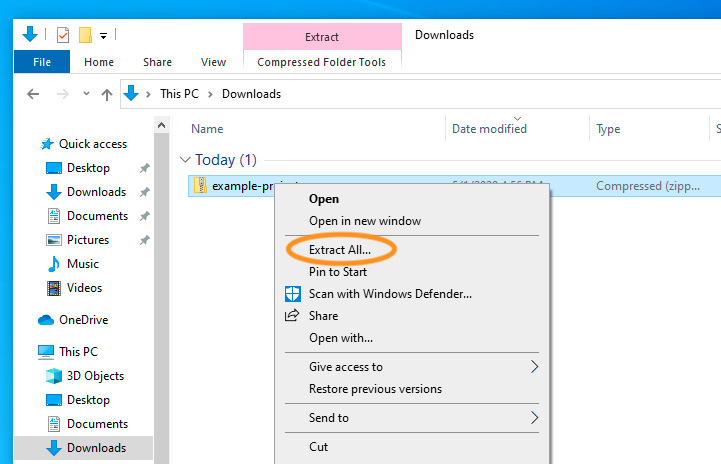
\includegraphics[width=0.6\textwidth,height=\textheight]{pics/extract-windows-1.png}

Then choose where you want to unzip all the files and click on
``Extract''

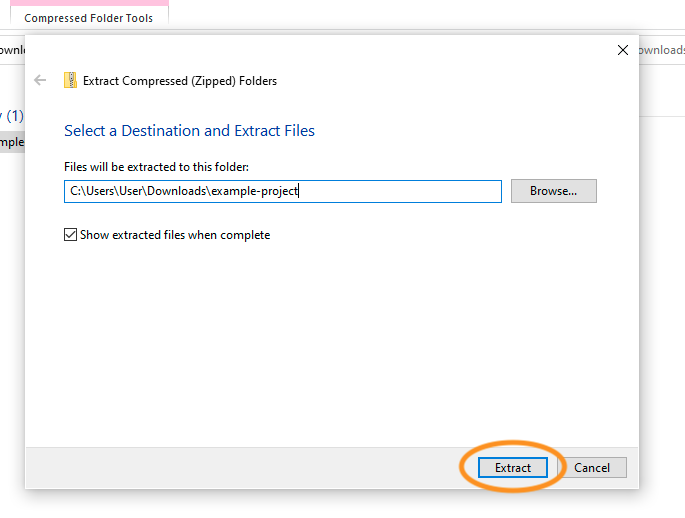
\includegraphics[width=0.6\textwidth,height=\textheight]{pics/extract-windows-2.png}

You should then finally have a real folder with all the contents of the
zipped file. Open the R Project file and RStudio will point to the
correct working directory and everything will work.

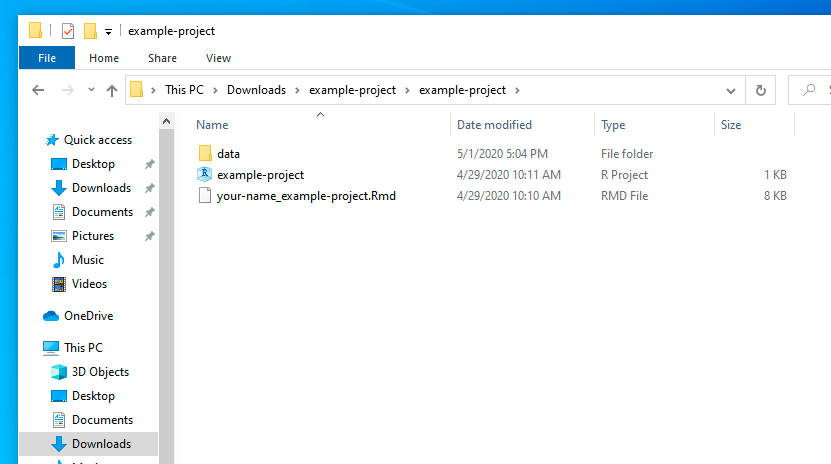
\includegraphics[width=0.6\textwidth,height=\textheight]{pics/extract-windows-3.png}

\bookmarksetup{startatroot}

\hypertarget{installing-r}{%
\chapter{Installing R}\label{installing-r}}

\begin{tcolorbox}[enhanced jigsaw, breakable, opacitybacktitle=0.6, colframe=quarto-callout-important-color-frame, bottomrule=.15mm, opacityback=0, toprule=.15mm, coltitle=black, toptitle=1mm, colback=white, titlerule=0mm, bottomtitle=1mm, colbacktitle=quarto-callout-important-color!10!white, title=\textcolor{quarto-callout-important-color}{\faExclamation}\hspace{0.5em}{Important Note Regarding Chromebooks}, rightrule=.15mm, arc=.35mm, leftrule=.75mm, left=2mm]

If you have a
\href{https://en.wikipedia.org/wiki/Chromebook}{Chromebook} rather than
a Windows or Mac computer, these installation instructions will not
work. While there are ways to install R, RStudio, and other software on
Chromebooks the process for doing so is different depending on what
version of ChromeOS you have and may not be supported on older models.
If this problem applies to you, please make an appointment or come by
during office hours as soon as possible so we can figure out what the
appropriate steps to get everything up and running are.

\end{tcolorbox}

The easiest way to install \texttt{R} is to go to
\href{https://cran.rstudio.com/}{this website} and select the operating
system you use.

For Mac users it is important to select the correct download for your
chip. If you are unsure click on the Apple logo in the top left of your
screen and then click about this Mac.

\begin{figure}

{\centering 
\includegraphics{figs/machine-image.png}

}

\caption{Look out for what chip your machine uses}

\end{figure}

I would download the one that says arm64. If your chip says ``intel
something or other'' then you would click on the one that says Intel
Macs.

\begin{tcolorbox}[enhanced jigsaw, breakable, opacitybacktitle=0.6, colframe=quarto-callout-important-color-frame, bottomrule=.15mm, opacityback=0, toprule=.15mm, coltitle=black, toptitle=1mm, colback=white, titlerule=0mm, bottomtitle=1mm, colbacktitle=quarto-callout-important-color!10!white, title=\textcolor{quarto-callout-important-color}{\faExclamation}\hspace{0.5em}{XQuartz for MacOS Users}, rightrule=.15mm, arc=.35mm, leftrule=.75mm, left=2mm]

If you downloaded either of the MacOS versions above, you also need to
\href{https://www.xquartz.org/}{download and install XQuartz}.
\textbf{This step is only for MacOS users}.

\end{tcolorbox}

For Windows \href{https://cran.rstudio.com/bin/windows/base/}{please
click on this link} and
\href{https://support.microsoft.com/en-us/topic/update-for-universal-c-runtime-in-windows-c0514201-7fe6-95a3-b0a5-287930f3560c}{then
follow this link} and download the appropriate version of the software
for your operating system. To check whether you need the X64 version or
the X86 version press the windows + x keys and then click on system. You
are looking for something that looks like this

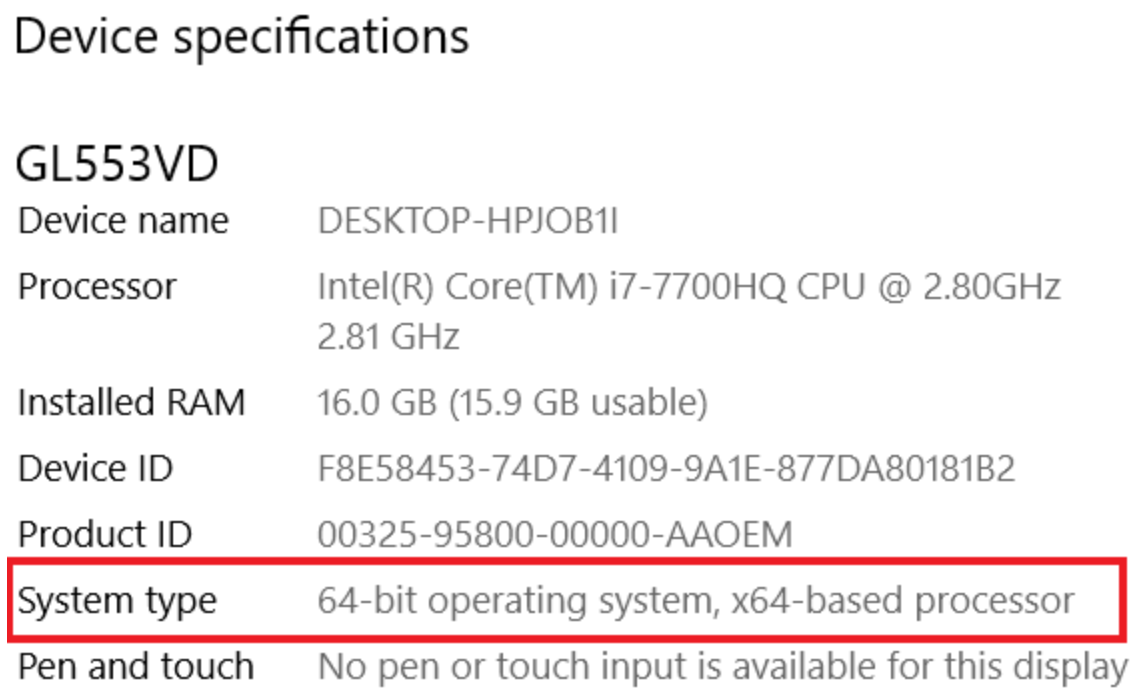
\includegraphics{figs/windows-machine.png}

Then choose 64 or 86.

\hypertarget{r-tools-and-xcode}{%
\section{R Tools and XCode}\label{r-tools-and-xcode}}

Occasionally some of the packages we will use may not be available for
your version of R. This is not a problem since many package writers have
the code online and we need to download them. This does require we have
some additional things on our computer.

\subsection{Windows}

\begin{tcolorbox}[enhanced jigsaw, breakable, opacitybacktitle=0.6, colframe=quarto-callout-warning-color-frame, bottomrule=.15mm, opacityback=0, toprule=.15mm, coltitle=black, toptitle=1mm, colback=white, titlerule=0mm, bottomtitle=1mm, colbacktitle=quarto-callout-warning-color!10!white, title=\textcolor{quarto-callout-warning-color}{\faExclamationTriangle}\hspace{0.5em}{Required Step}, rightrule=.15mm, arc=.35mm, leftrule=.75mm, left=2mm]

For some of the packages we will need we may need to have some
additional things installed in order for it to work.

\end{tcolorbox}

If you are on a Windows operating system, you will need to install
\href{https://cran.r-project.org/bin/windows/Rtools/rtools43/rtools.html}{Rtools
4.3} which can download by clicking on the hyperlink below. Rtools is
required to install packages from source and, more importantly, anything
that requires a C++ compiler.

\begin{itemize}
\tightlist
\item
  \href{https://cran.r-project.org/bin/windows/Rtools/rtools43/files/rtools43-5550-5548.exe}{Download
  Rtools 4.3}
\end{itemize}

Once again, during the installation process you can just leave things at
their default settings, especially in the case of the installation
directory since changing its default locations may result in errors
during package compilation. After you have completed this step, you will
need to install the required packages by running the code below in order
to successfully render the Quarto document for problem set 0. \textbf{If
you encounter errors when rendering the document, please ensure you have
these packages installed.}

\subsection{MacOS}

\begin{tcolorbox}[enhanced jigsaw, breakable, opacitybacktitle=0.6, colframe=quarto-callout-warning-color-frame, bottomrule=.15mm, opacityback=0, toprule=.15mm, coltitle=black, toptitle=1mm, colback=white, titlerule=0mm, bottomtitle=1mm, colbacktitle=quarto-callout-warning-color!10!white, title=\textcolor{quarto-callout-warning-color}{\faExclamationTriangle}\hspace{0.5em}{Required Step}, rightrule=.15mm, arc=.35mm, leftrule=.75mm, left=2mm]

For some of the packages we will need we may need to have some
additional things installed in order for it to work. This is a required
step for much of the code we will use throughout this course.

\end{tcolorbox}

If you are on a MacOS operating system, you will need to install the
Xcode developer tools. You can obtain the full MacOS development
environment from the
\href{https://developer.apple.com/xcode/resources/}{Apple AppStore}
using the link below. Xcode is required to install packages from source
and, more importantly, anything that requires a C++ compiler, including
though not limited to Stan.

\begin{itemize}
\tightlist
\item
  \href{https://apps.apple.com/us/app/xcode/id497799835?mt=12}{Download
  Xcode from the AppStore}
\end{itemize}

However, since downloading this can be extremely time consuming given
the large size of the full development tools suite an alternative option
is to install a paired down version that provides the tools necessary
for our purposes in this course without the overhead of the full Xcode
development environment. You can install the paired down version of
Xcode by running the code below in the RStudio console. Just copy and
paste and hit enter.

\begin{Shaded}
\begin{Highlighting}[]
\DocumentationTok{\#\# MacOS Users may need to install the rstudioapi manually first}
\FunctionTok{install.packages}\NormalTok{(}\StringTok{"rstudioapi"}\NormalTok{)}

\DocumentationTok{\#\# Run the command to install xcode{-}select}
\NormalTok{rstudioapi}\SpecialCharTok{::}\FunctionTok{terminalExecute}\NormalTok{(}
  \AttributeTok{command =} \StringTok{"xcode{-}select {-}{-}install"}
\NormalTok{)}
\end{Highlighting}
\end{Shaded}

\hypertarget{quarto}{%
\section{Quarto}\label{quarto}}

If you have read through the course syllabus you will notice that I am
having you work in something called Quarto. You may be asking your self
what is Quarto I have only used MS Word. Quarto embraces something
called literate programming. Essentially what this means is that words
and code appear side by side. This guide was created in Quarto and what
I use the most. Since we are going to produce lots of graphs and tables
in this class the typical workflow for that would look something like
this

\begin{figure}

{\centering 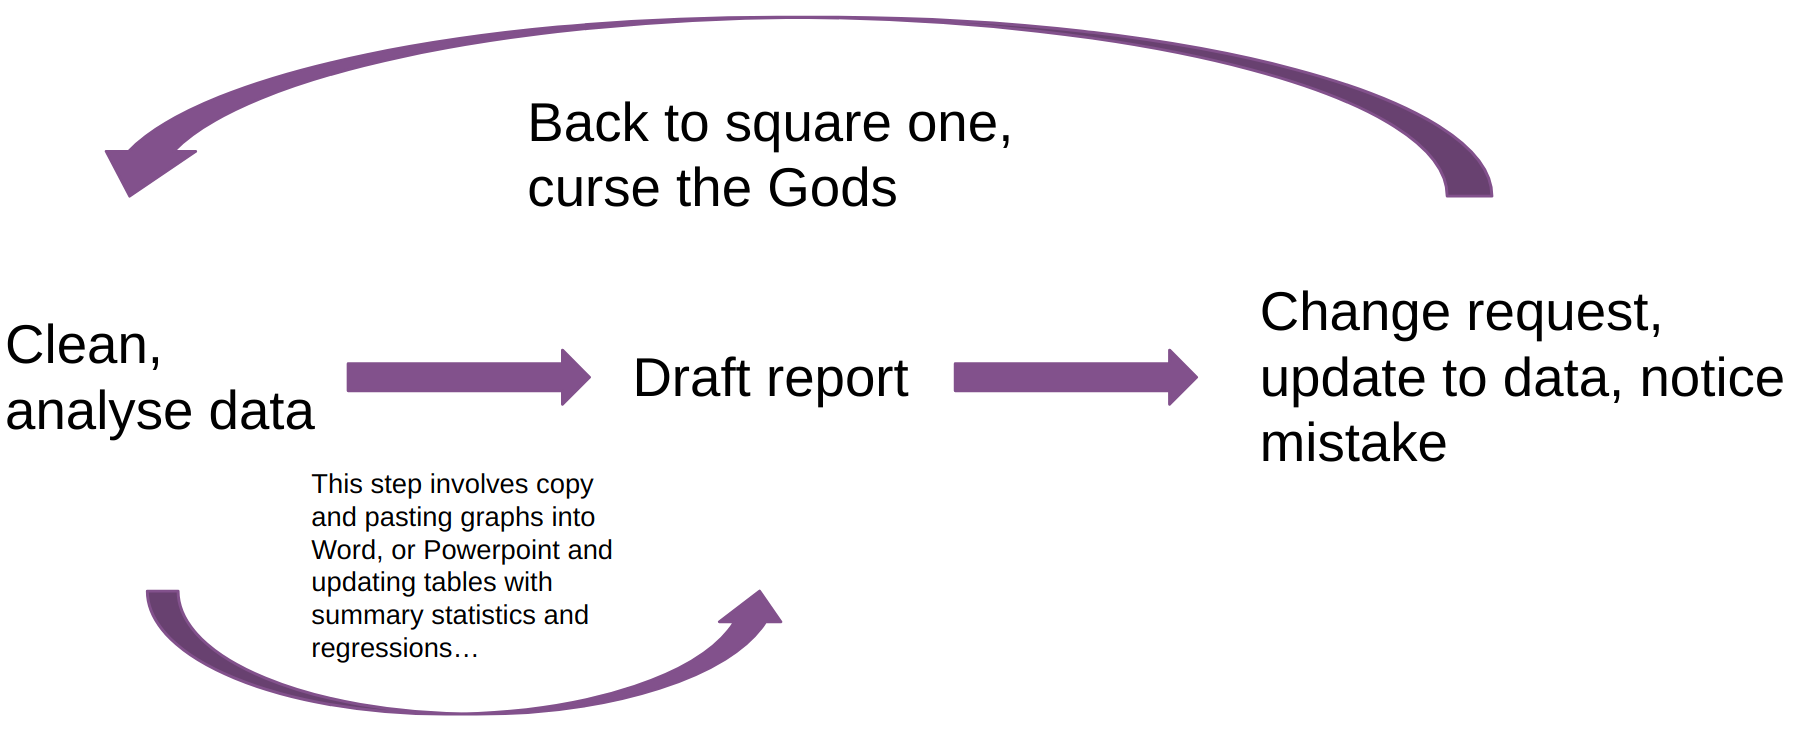
\includegraphics[width=5.98in,height=\textheight]{figs/report_draft_loop.png}

}

\caption{Credit for this image goes to Bruno Rodrigues}

\end{figure}

This involves lots of work for yourself. If you are doing a data
analysis project where you produce 5 plots each time you make minor
changes to those plots you are going to have to remember where those
plots are, copy and paste them over, resize them or reformat them. This
gets infinitely more annoying if you are reporting numbers in tables or
in text. In some cases data analysis teams are constantly updating
reports for stake holders based on new data. So if you have a report
that says our ``based on our model we would expect an increase of 8 blah
blahs'' and later you rerun the analysis cuz there was new data or you
notice a mistake you have to figure out where exactly you said ``8 blah
blahs'' and switch them.

In Quarto this process is a whole lot easier. The loop looks like this

\begin{figure}

{\centering 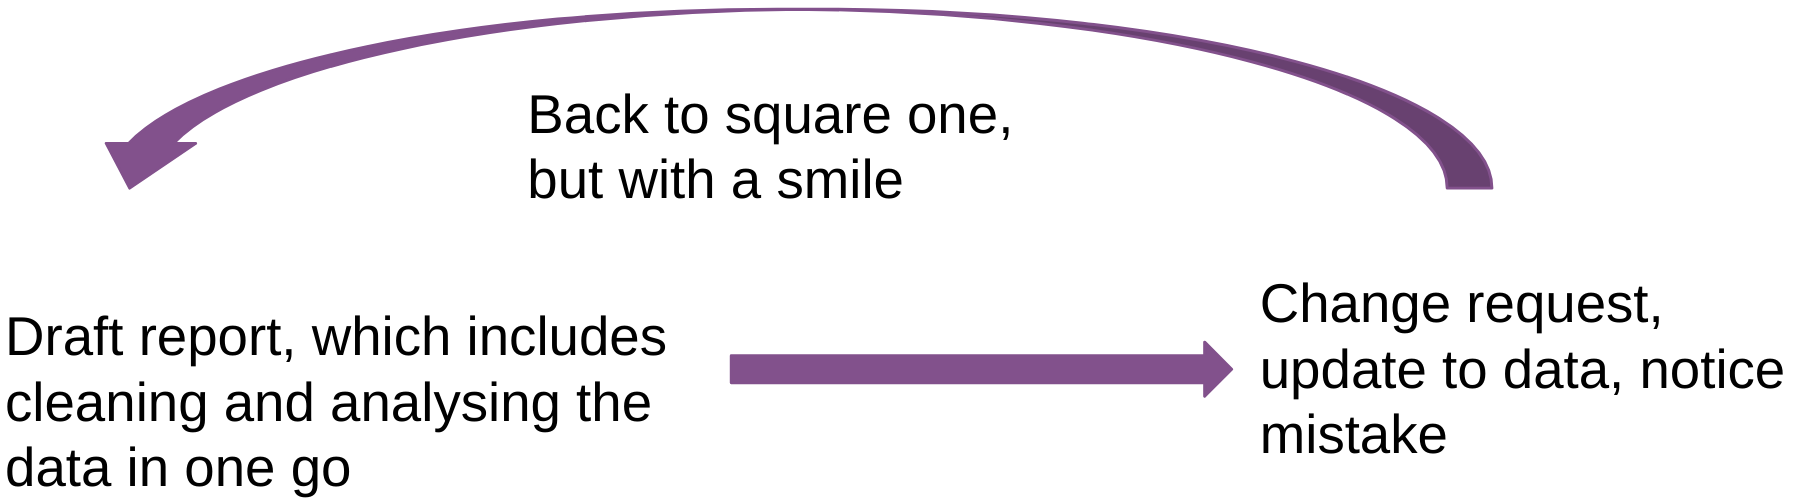
\includegraphics[width=6in,height=\textheight]{figs/md_draft_loop.png}

}

\caption{Credit for this image goes to Bruno Rodrigues}

\end{figure}

You are changing the code for your figures in the document itself. So
any changes are going to appear in the document automatically! You can
also use code inline to automatically update numbers!

\begin{Shaded}
\begin{Highlighting}[]
\NormalTok{data }\OtherTok{\textless{}{-}} \DecValTok{1}\SpecialCharTok{:}\DecValTok{100}

\NormalTok{avg }\OtherTok{\textless{}{-}} \FunctionTok{mean}\NormalTok{(data)}
\end{Highlighting}
\end{Shaded}

The average for our data is 50.5. In the document it looks like this

\begin{Shaded}
\begin{Highlighting}[]

\InformationTok{\textasciigrave{}\textasciigrave{}\textasciigrave{}\{r\}}
\NormalTok{data }\OtherTok{\textless{}{-}} \DecValTok{1}\SpecialCharTok{:}\DecValTok{100}

\NormalTok{avg }\OtherTok{\textless{}{-}} \FunctionTok{mean}\NormalTok{(data)}

\InformationTok{\textasciigrave{}\textasciigrave{}\textasciigrave{}}


\NormalTok{The average of our data is }\InformationTok{\textasciigrave{}r avg\textasciigrave{}}
\end{Highlighting}
\end{Shaded}

You may have noticed that our data only goes from 1 to 100. We can make
a quick modification and the document will update the document
accordingly without any copy and pasting!

\begin{Shaded}
\begin{Highlighting}[]
\NormalTok{data }\OtherTok{\textless{}{-}} \DecValTok{1}\SpecialCharTok{:}\DecValTok{1000}

\NormalTok{avg }\OtherTok{\textless{}{-}} \FunctionTok{mean}\NormalTok{(data)}
\end{Highlighting}
\end{Shaded}

The average of our data is 500.5

\hypertarget{navigating-rstudio}{%
\section{Navigating Rstudio}\label{navigating-rstudio}}

\hypertarget{r-rstudio-whats-the-difference}{%
\subsection{R? Rstudio? Whats the
Difference?}\label{r-rstudio-whats-the-difference}}

\begin{itemize}
\tightlist
\item
  R is a statistical programming language
\item
  RStudio is a convenient interface for R (an Integrated Developer
  Environment, IDE)
\item
  At its simplest:

  \begin{itemize}
  \tightlist
  \item
    R is like a car's engine
  \item
    RStudio is like a car's dashboard
  \end{itemize}
\end{itemize}

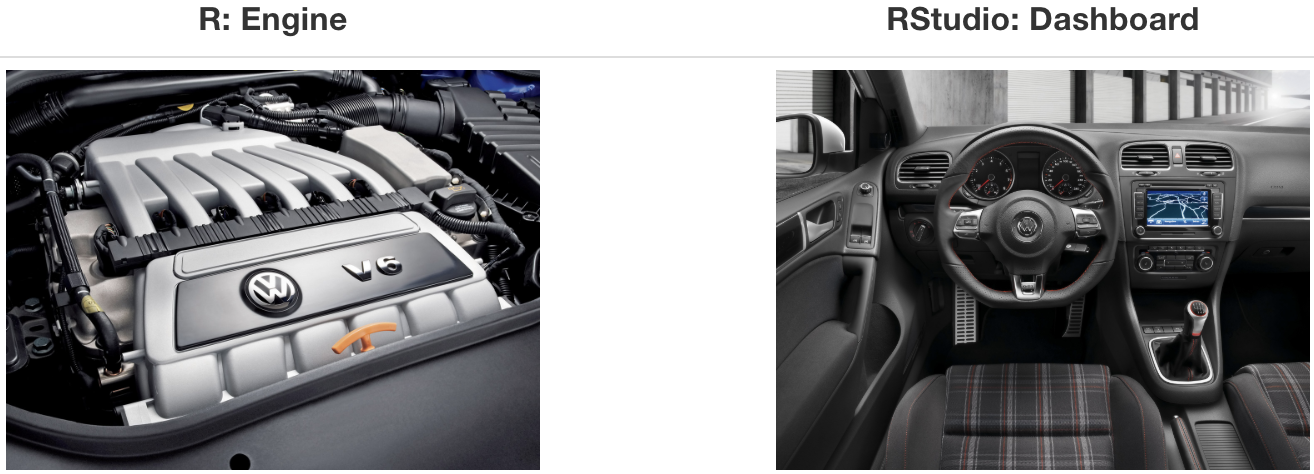
\includegraphics[width=4.38in,height=\textheight]{pics/engine-dashboard.png}

The most common way that we interact with R is through Rstudio you can
technically run R by just opening R and typing in code. But most people
do not do this. It is not especially friendly to work in there is no
syntax highlighting no code completetion. There isnt even really an
option to add keyboard shortcuts. It is kind of like a Formula 1 car it
can go real fast but it is not a comfortable drive.

Rstudio has lots of handy features that help you. Much like a car you
and I would drive. If we didn't have the dashboard but still had the
engine and some wheels and a steering we could drive the car if needed.
However a car with a dashboard lets us figure out what the car is doing
more easily.

\hypertarget{navigating-rstudio-1}{%
\subsection{Navigating RStudio}\label{navigating-rstudio-1}}

When you open up Rstudio it should look something like this.

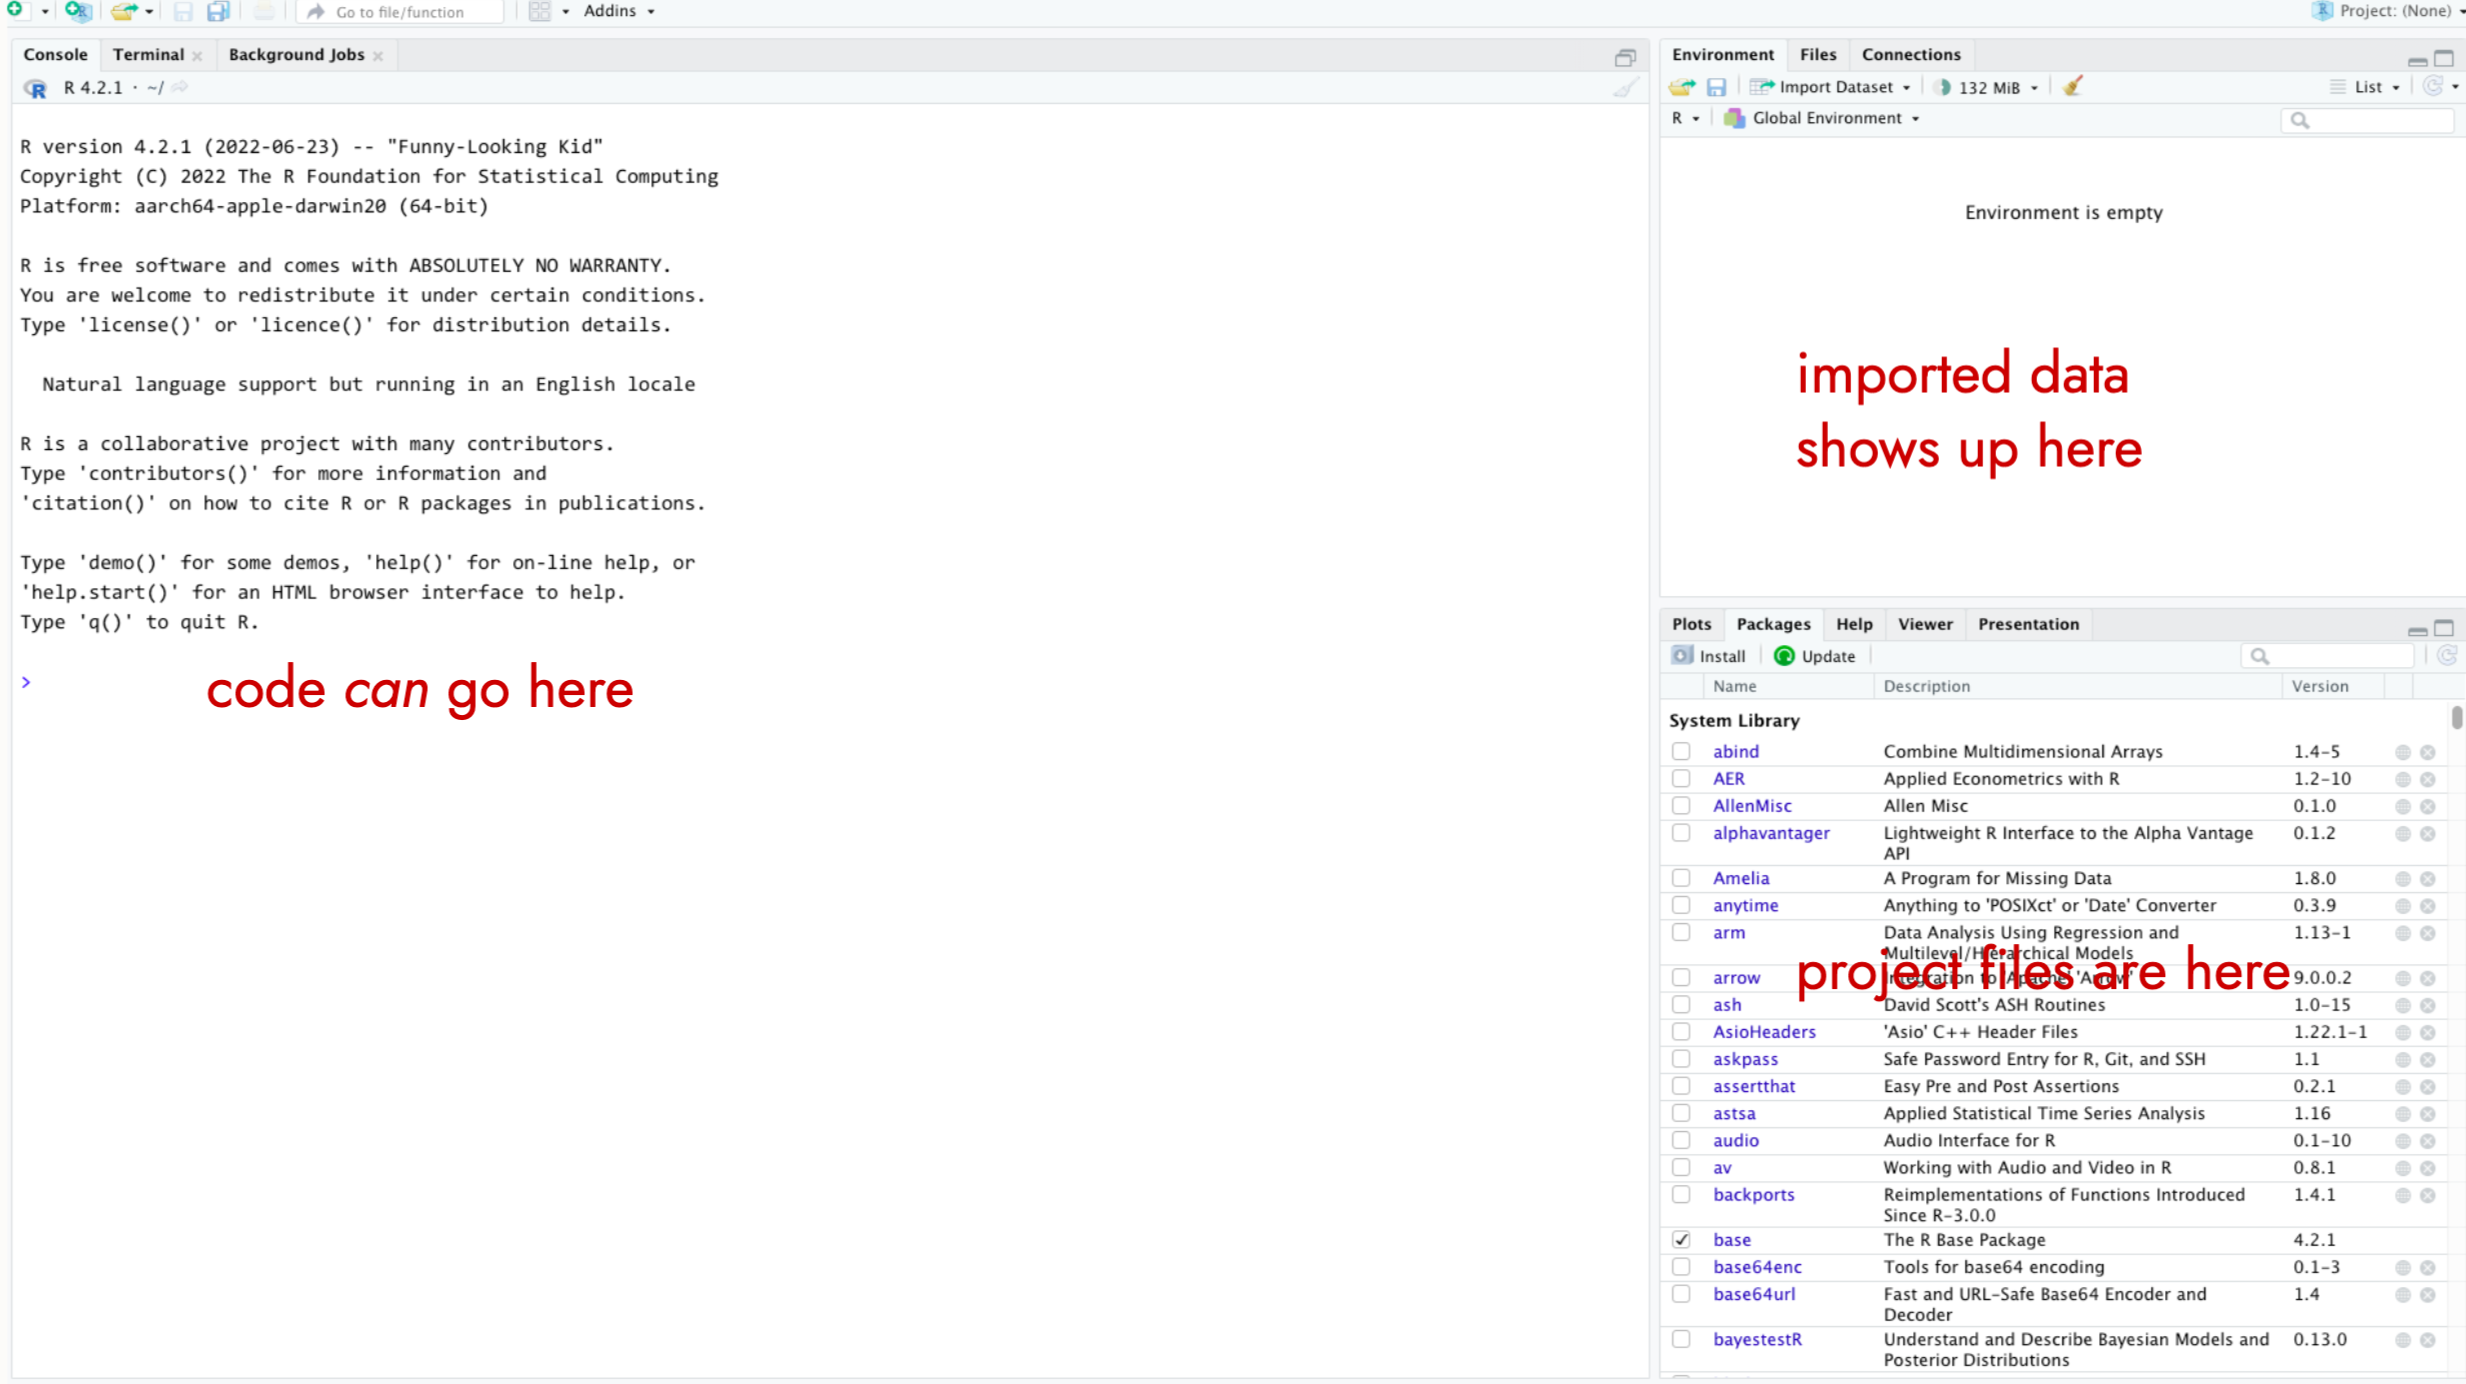
\includegraphics[width=8.22in,height=\textheight]{figs/annotated-rstudio.png}

It is worth briefly walking through each pane. The code can go here part
is called the \texttt{console}. If you just start typing R code and hit
enter it will run. The \texttt{imported\ data\ shows\ up\ here} lets us
peak at our \texttt{Global\ Environment}. This is where stuff we
need/worked on shows up. \texttt{Project\ files\ are\ here} in the
bottom right actually has a lot of panes there. The first one called
\texttt{files} lets us peak at all the files in the folder that R is
pointed at. The second pane \texttt{packages} lets us look at all the
packages we have installed(more on this later). \texttt{Plots} lets us
preview plots we have made.

Most of the time we don't enter code directly into the console. If we
just enter code into the console we do not have a record of what we did!
This is a bad workflow for lots of reasons! At a minimum you are making
your life a whole lot more difficult because you will have to redo
everything every single time. That is way more work for yourself. If you
click on the little white page at the top left you will see something
that looks like this.

\begin{figure}

{\centering 
\includegraphics[width=0.77in,height=\textheight]{figs/rscript-open.png}

}

\end{figure}

This is a fairly standard way to store your code! This is a record of
everything you did which is really important because it saves you time.
Just as importantly it lets your colleagues see what you did to the
data. If we don't know what you did than it is hard to know where things
are going wrong or if what you did matches what you said.

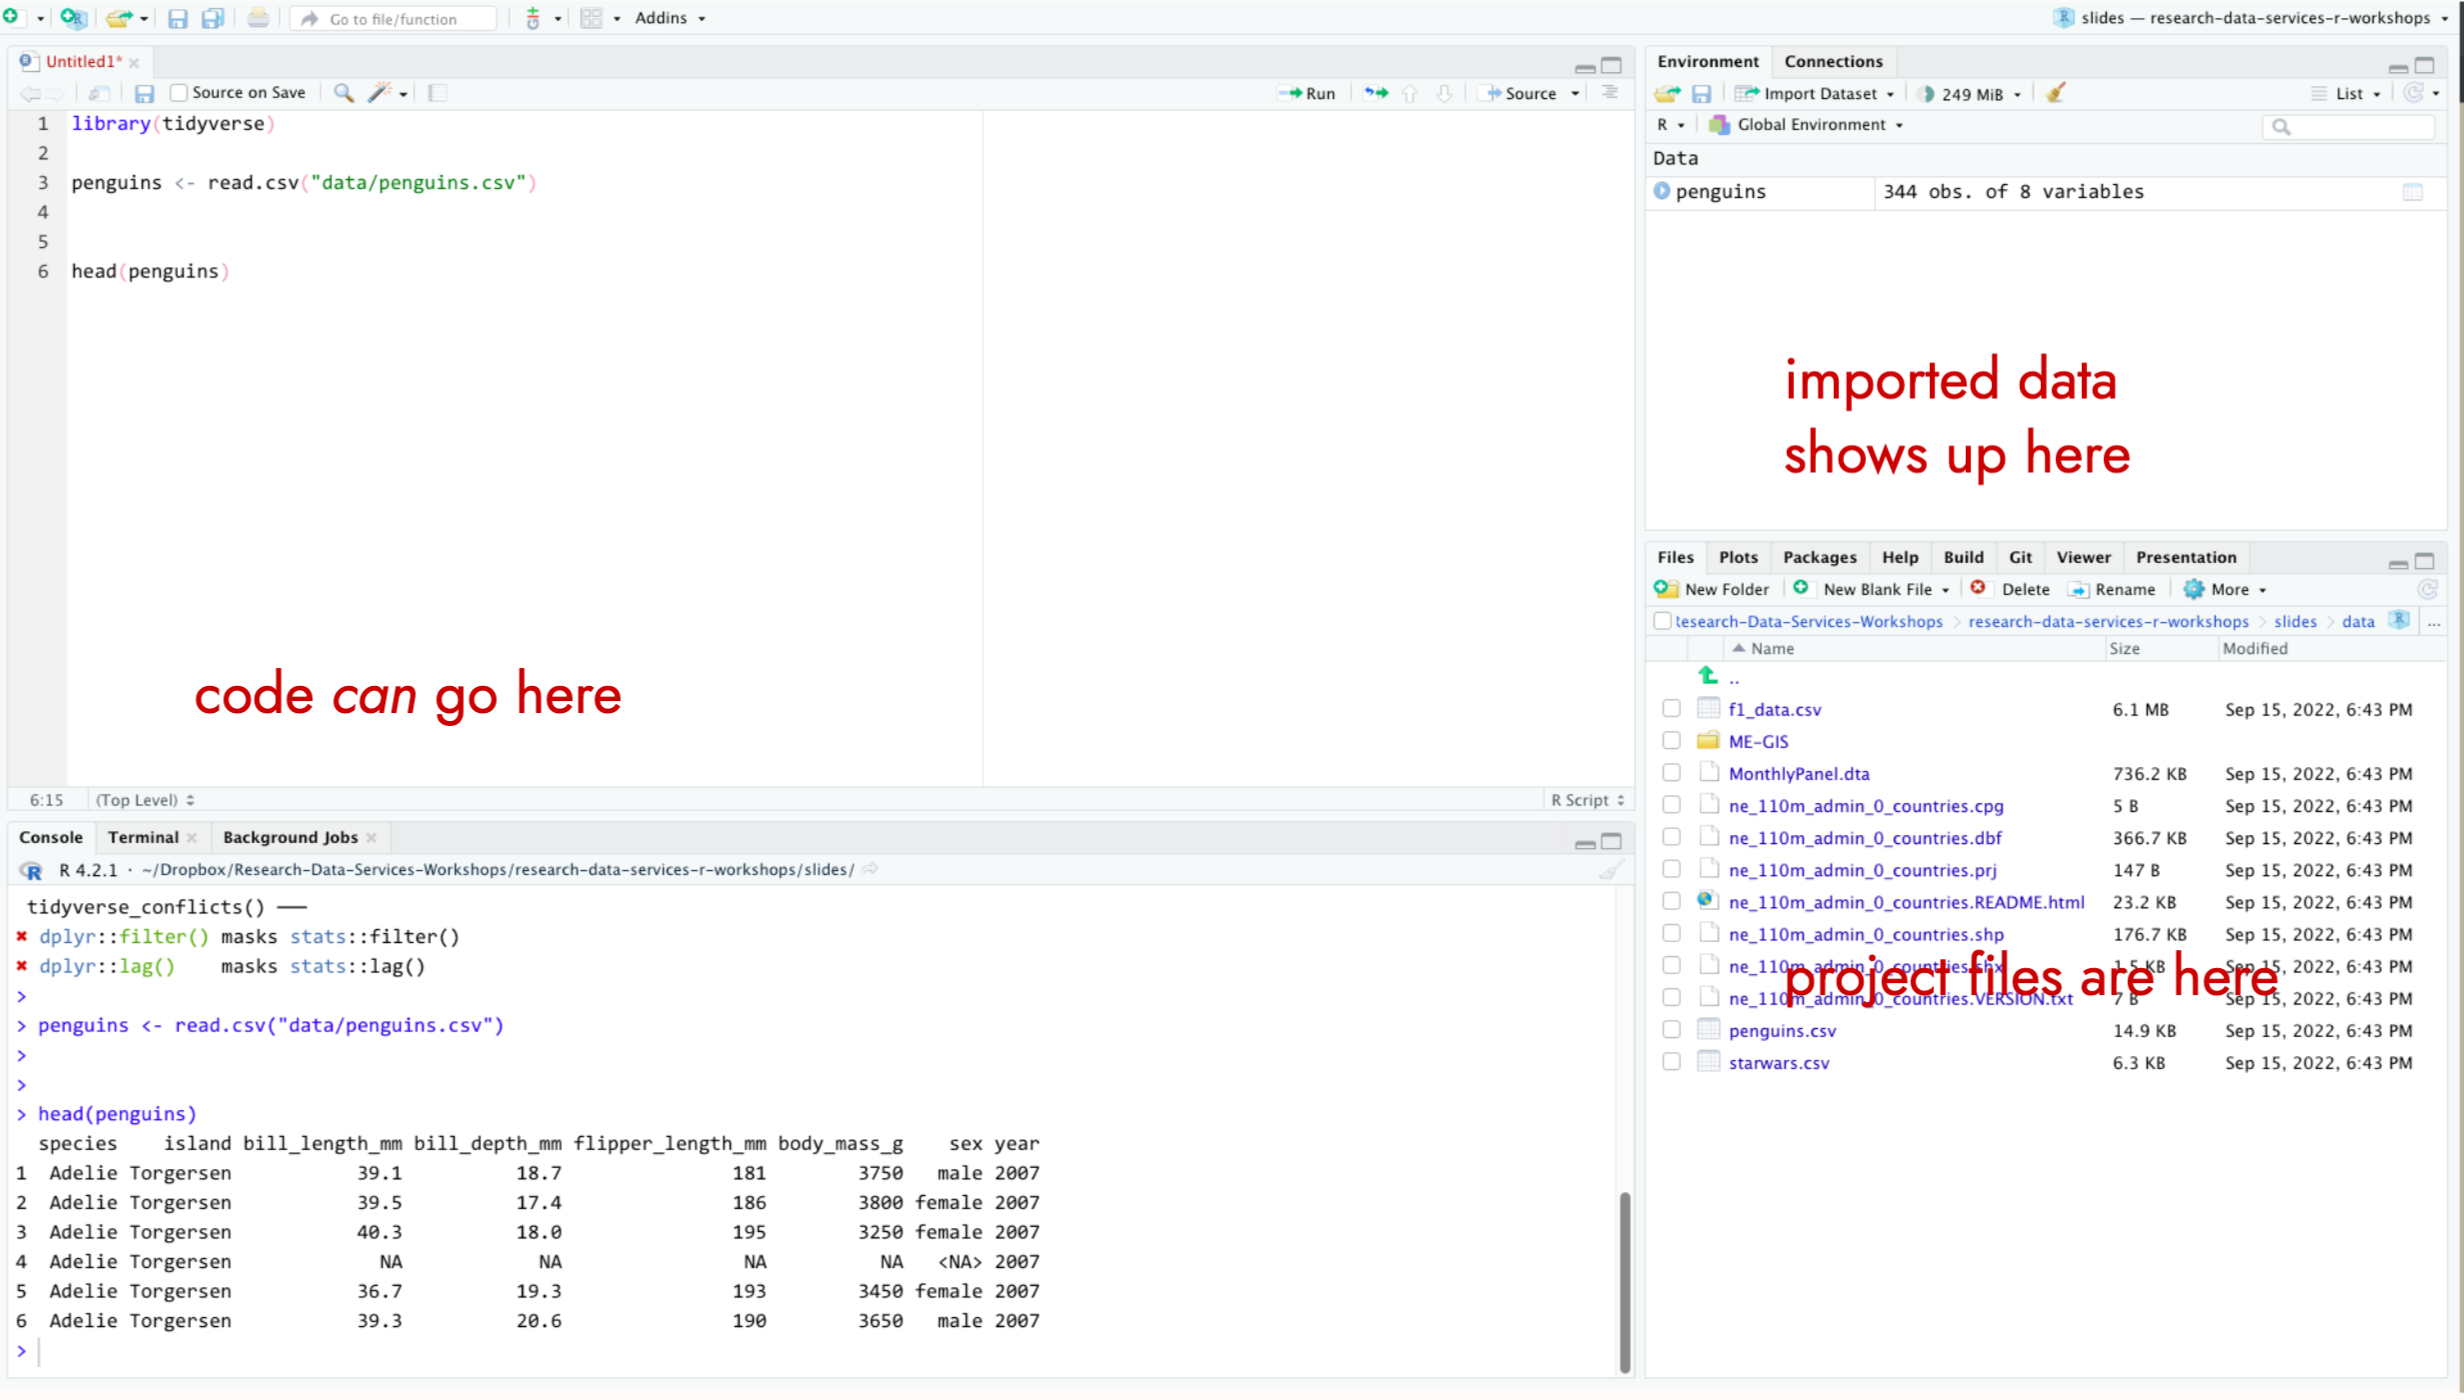
\includegraphics[width=8.21in,height=\textheight]{figs/annotate-two-r.png}

If you opened an R script than it should look something like this. If
you highlight the code and hit \texttt{cmd\ +\ enter} on a Mac or
\texttt{ctrl\ +\ enter} if you are on a Windows then it will run the
code for you!

Now that you have R Studio and R all set lets get started on the basics
of R!

\bookmarksetup{startatroot}

\hypertarget{basics-of-r}{%
\chapter{Basics of R}\label{basics-of-r}}

In this chapter I will introduce you to the basics of R and object
oriented programming. These may be relatively new concepts for you and
thats okay! I encourage you to follow along in Rstudio. Open up an R
script and either type in the code

\hypertarget{r-as-a-fancy-calculator}{%
\section{R as a fancy calculator}\label{r-as-a-fancy-calculator}}

Good news you never have to buy a TI-84 again you can use R as a fancy
calculator.

\begin{Shaded}
\begin{Highlighting}[]
\DecValTok{2}\SpecialCharTok{+}\DecValTok{2} \DocumentationTok{\#\# addition}
\end{Highlighting}
\end{Shaded}

\begin{verbatim}
[1] 4
\end{verbatim}

\begin{Shaded}
\begin{Highlighting}[]
\DecValTok{4{-}2} \DocumentationTok{\#\# subtraction}
\end{Highlighting}
\end{Shaded}

\begin{verbatim}
[1] 2
\end{verbatim}

\begin{Shaded}
\begin{Highlighting}[]
\DecValTok{600}\SpecialCharTok{*}\DecValTok{100} \DocumentationTok{\#\#multiplication}
\end{Highlighting}
\end{Shaded}

\begin{verbatim}
[1] 60000
\end{verbatim}

\begin{Shaded}
\begin{Highlighting}[]
\DecValTok{100}\SpecialCharTok{/}\DecValTok{10} \DocumentationTok{\#\#division}
\end{Highlighting}
\end{Shaded}

\begin{verbatim}
[1] 10
\end{verbatim}

\begin{Shaded}
\begin{Highlighting}[]
\DecValTok{10}\SpecialCharTok{*}\DecValTok{10}\SpecialCharTok{/}\NormalTok{(}\DecValTok{3}\SpecialCharTok{\^{}}\DecValTok{4}\SpecialCharTok{*}\DecValTok{2}\NormalTok{)}\SpecialCharTok{{-}}\DecValTok{2} \DocumentationTok{\#\# Pemdas }
\end{Highlighting}
\end{Shaded}

\begin{verbatim}
[1] -1.382716
\end{verbatim}

\begin{Shaded}
\begin{Highlighting}[]
\FunctionTok{log}\NormalTok{(}\DecValTok{100}\NormalTok{) }\CommentTok{\# takes the log of 100}
\end{Highlighting}
\end{Shaded}

\begin{verbatim}
[1] 4.60517
\end{verbatim}

\begin{Shaded}
\begin{Highlighting}[]
\FunctionTok{sqrt}\NormalTok{(}\DecValTok{100}\NormalTok{) }\CommentTok{\# sqrt of 100}
\end{Highlighting}
\end{Shaded}

\begin{verbatim}
[1] 10
\end{verbatim}

However, if we want to reuse stuff we need to \textbf{assign them} to an
object. This applies for all the numbers we calculated above and datsets
you read in! This is somewhat unintuitive if you have never worked with
an object oriented program. However, you will eventually get the hang of
it!

\hypertarget{objects}{%
\section{Objects}\label{objects}}

\hypertarget{objects-and-assignment}{%
\subsection{Objects and Assignment}\label{objects-and-assignment}}

In the installation chapter I showed did some assigning without really
telling you, but now it is time to explain what is going on. R is what
is known as an
\href{https://en.wikipedia.org/wiki/Object-oriented_programming}{object
oriented programming language (OOP)}, meaning that everything in R is an
``object.'' This is useful for understanding the concept of
\emph{assignment}, or how we specify certain objects in memory so we can
use them elsewhere in a script. Values need to be assigned to objects
using the assignment operator \texttt{\textless{}-},
\texttt{\textless{}} followed by \texttt{-}, and then on the right side
you tell R what goes in that object. This can be as simple as specifying
a calculation such as \texttt{4\ +\ 4} or passing numeric values to a
function such as \texttt{sum(9,\ 6)}.

\begin{tcolorbox}[enhanced jigsaw, breakable, opacitybacktitle=0.6, colframe=quarto-callout-tip-color-frame, bottomrule=.15mm, opacityback=0, toprule=.15mm, coltitle=black, toptitle=1mm, colback=white, titlerule=0mm, bottomtitle=1mm, colbacktitle=quarto-callout-tip-color!10!white, title=\textcolor{quarto-callout-tip-color}{\faLightbulb}\hspace{0.5em}{Tip}, rightrule=.15mm, arc=.35mm, leftrule=.75mm, left=2mm]

The keyboard shortcut for \texttt{\textless{}-} is \texttt{alt\ +\ -}

\end{tcolorbox}

\begin{Shaded}
\begin{Highlighting}[]
\NormalTok{numbs }\OtherTok{\textless{}{-}} \DecValTok{4} \SpecialCharTok{+} \DecValTok{4} 

\NormalTok{chars }\OtherTok{\textless{}{-}} \StringTok{"hello world"}

\NormalTok{numbs2 }\OtherTok{\textless{}{-}} \DecValTok{3}\SpecialCharTok{*}\DecValTok{3}

\NormalTok{numbs }\SpecialCharTok{+}\NormalTok{ numbs2}
\end{Highlighting}
\end{Shaded}

\begin{verbatim}
[1] 17
\end{verbatim}

When we assign things the resulting values are not returned so we can
``print'' the object explicitly using \texttt{print} or referring to it
by name.

\begin{Shaded}
\begin{Highlighting}[]
\FunctionTok{print}\NormalTok{(numbs)}
\end{Highlighting}
\end{Shaded}

\begin{verbatim}
[1] 8
\end{verbatim}

\begin{Shaded}
\begin{Highlighting}[]
\NormalTok{chars }
\end{Highlighting}
\end{Shaded}

\begin{verbatim}
[1] "hello world"
\end{verbatim}

One fairly common error you will run into in \texttt{R} is something
along this line.

\begin{Shaded}
\begin{Highlighting}[]
\NormalTok{chars\_two }\OtherTok{\textless{}{-}} \StringTok{"Tell Cersei it was me"}

\NormalTok{charstwo}
\end{Highlighting}
\end{Shaded}

\begin{verbatim}
Error in eval(expr, envir, enclos): object 'charstwo' not found
\end{verbatim}

While this is a fairly minor typo if we look at the global environment
we will get a hint.

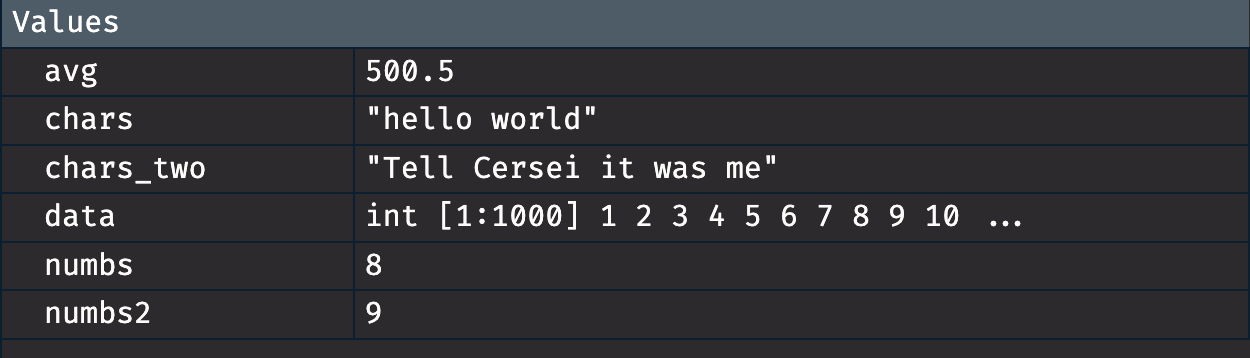
\includegraphics{figs/environment-no-data.png}

When we asked \texttt{R} to print \texttt{charstwo} it is going to look
in the global environment for something called \texttt{charstwo} to
print and if it can't find it then R will give up. We don't have
anything called \texttt{charstwo} but we do have something called
\texttt{chars\_two}. We know what we meant when we made the typo, but
the computer does not! Computers are really good at doing things, but
they require really explicit instructions so if we type
\texttt{chars\_two} it will work.

\begin{Shaded}
\begin{Highlighting}[]
\NormalTok{chars\_two}
\end{Highlighting}
\end{Shaded}

\begin{verbatim}
[1] "Tell Cersei it was me"
\end{verbatim}

One way to make life a little bit is have a consistent naming
convention! This will generally help you because you will develop some
tendencies. However, this is an error we all still get because it is
easy to forget what all your objects are named. You can either look at
your global environment or scroll up and see what past you named the
object.

\hypertarget{naming-objects-in-r}{%
\subsection{Naming Objects in R}\label{naming-objects-in-r}}

The best practice is to use concise descriptive names.

When loading in data typically I do \texttt{raw\_my\_dataset\_name} and
after data all of my cleaning I do \texttt{clean\_my\_dataset\_name}

\begin{itemize}
\tightlist
\item
  Objects must start with a letter. But can contain letters, numbers,
  \texttt{\_}, or \texttt{.} There are a few different naming
  conventions that people use.

  \begin{itemize}
  \tightlist
  \item
    snake\_case\_like\_this\_is\_what\_I\_use
  \item
    somePeopleUseCamelCase
  \item
    some\_People.are\_Do\_not.like\_Convention\footnote{Example and
      Discussion provided in
      \href{https://r4ds.had.co.nz/workflow-basics.html?q=snake\#\#whats-in-a-name}{R
      for Data Sciency} by Hadley Wickham}
  \end{itemize}
\end{itemize}

\hypertarget{things-we-can-never-name-stuff-in-r}{%
\subsection{Things we can never name stuff in
R}\label{things-we-can-never-name-stuff-in-r}}

\section{if/else}

\texttt{if} used when something meets a certain condition the code will
do something. \texttt{else} is used when the if condition is not met

\section{for/while}

\texttt{for} is how we construct something called a for loop.
\texttt{while} is used to construct something called a while loop. These
are ways to repeat the same task over and over again and are building
blocks of packages in R.

\section{function}

How we specify user defined functions. This is building block of
programming in R

\section{TRUE/FALSE}

Logical constants in R

\section{NULL}

is returned when an expression or function results in an undefined value

\section{Inf/-Inf}

This is way R represents you doing something mathematically impossible
like 1/0 or \texttt{log(0)}

\section{NaN}

This is a way R represents you doing something mathematically impossible
like 0/0. NaN stands for not a real number

\section{NA}

This is the most common way that R represents missing values

\marginnote{\begin{footnotesize}

Sometimes you will run into names that do not follow naming conventions
so if you name something \texttt{my\ object\ name} \texttt{R} will get
mad about it so you have you use two ` (the key right beside 1) like
this.

\begin{Shaded}
\begin{Highlighting}[]
\StringTok{\textasciigrave{}}\AttributeTok{my object name}\StringTok{\textasciigrave{}}
\end{Highlighting}
\end{Shaded}

\end{footnotesize}}

\hypertarget{types-of-objects-in-r}{%
\section{\texorpdfstring{Types of Objects in
\texttt{R}}{Types of Objects in R}}\label{types-of-objects-in-r}}

Before we can proceed to a functional programming framework, however, it
is first necessary to introduce the basic data structures you will
encounter in R. These include, though are not limited to
\href{https://r4ds.had.co.nz/tibbles.html}{data frames},
\href{https://r4ds.had.co.nz/factors.html}{factors},
\href{https://r4ds.had.co.nz/vectors.html}{vectors},
\href{https://r4ds.had.co.nz/vectors.html?q=list\#lists}{lists}, and
\href{https://r4ds.had.co.nz/functions.html}{functions}. In this section
we will spend a brief amount of time introducing data structures with a
focus on vectors, data frames, lists, and functions in particular.

\hypertarget{vectors}{%
\subsection{Vectors}\label{vectors}}

If you look at our example, we are kind of repeating ourselves. What we
can do is to create what is called a vector using \texttt{c} which will
smash the numbs vector together. Vectors have lots of uses in R and can
make your life a lot easier. A vector comes in two flavors we will focus
on one of the two main types.

\begin{Shaded}
\begin{Highlighting}[]
\NormalTok{my\_vec }\OtherTok{\textless{}{-}} \FunctionTok{c}\NormalTok{(numbs, numbs2)}

\NormalTok{my\_vec}
\end{Highlighting}
\end{Shaded}

\begin{verbatim}
[1] 8 9
\end{verbatim}

\begin{Shaded}
\begin{Highlighting}[]
\NormalTok{my\_other\_vec }\OtherTok{\textless{}{-}} \FunctionTok{c}\NormalTok{(}\DecValTok{1}\SpecialCharTok{:}\DecValTok{100}\NormalTok{)}

\NormalTok{my\_other\_vec}
\end{Highlighting}
\end{Shaded}

\begin{verbatim}
  [1]   1   2   3   4   5   6   7   8   9  10  11  12  13  14  15  16  17  18
 [19]  19  20  21  22  23  24  25  26  27  28  29  30  31  32  33  34  35  36
 [37]  37  38  39  40  41  42  43  44  45  46  47  48  49  50  51  52  53  54
 [55]  55  56  57  58  59  60  61  62  63  64  65  66  67  68  69  70  71  72
 [73]  73  74  75  76  77  78  79  80  81  82  83  84  85  86  87  88  89  90
 [91]  91  92  93  94  95  96  97  98  99 100
\end{verbatim}

This is called an atomic vector. This is just computer science, for
everything in the vector is the same class. The class of an object tells
you what you can do and cannot do to stuff. To get the class of a
vector, you do something like this

\begin{Shaded}
\begin{Highlighting}[]
\FunctionTok{class}\NormalTok{(my\_vec)}
\end{Highlighting}
\end{Shaded}

\begin{verbatim}
[1] "numeric"
\end{verbatim}

\begin{Shaded}
\begin{Highlighting}[]
\FunctionTok{class}\NormalTok{(my\_other\_vec)}
\end{Highlighting}
\end{Shaded}

\begin{verbatim}
[1] "integer"
\end{verbatim}

Since this is a numeric variable we can do some math stuff to it. For
example we stored 8 in a vector called numbers. Lets add 8 to each
number in my\_other\_vec.

\begin{Shaded}
\begin{Highlighting}[]
\NormalTok{numbs }\SpecialCharTok{+}\NormalTok{ my\_other\_vec}
\end{Highlighting}
\end{Shaded}

\begin{verbatim}
  [1]   9  10  11  12  13  14  15  16  17  18  19  20  21  22  23  24  25  26
 [19]  27  28  29  30  31  32  33  34  35  36  37  38  39  40  41  42  43  44
 [37]  45  46  47  48  49  50  51  52  53  54  55  56  57  58  59  60  61  62
 [55]  63  64  65  66  67  68  69  70  71  72  73  74  75  76  77  78  79  80
 [73]  81  82  83  84  85  86  87  88  89  90  91  92  93  94  95  96  97  98
 [91]  99 100 101 102 103 104 105 106 107 108
\end{verbatim}

We can get the sum of the entire vector using the \texttt{sum} function

\begin{Shaded}
\begin{Highlighting}[]
\FunctionTok{sum}\NormalTok{(my\_other\_vec)}
\end{Highlighting}
\end{Shaded}

\begin{verbatim}
[1] 5050
\end{verbatim}

We can do this because these vectors have a class of numeric. What would
happen if we added our \texttt{chars} vector to our \texttt{numbs}
vector?

\begin{Shaded}
\begin{Highlighting}[]
\NormalTok{chars }\SpecialCharTok{+}\NormalTok{ numbs }
\end{Highlighting}
\end{Shaded}

\begin{verbatim}
Error in chars + numbs: non-numeric argument to binary operator
\end{verbatim}

Hopefully this error makes sense intuitevly. If we were in class and I
asked you to find the answer to \texttt{8\ \ +\ hello\ world} you would
rightfully be really confused. This is essentially what is going on with
\texttt{R}.

You can construct vectors with different kinds of stuff but it will lead
to some strange behavior.

\begin{Shaded}
\begin{Highlighting}[]
\NormalTok{examp\_weird }\OtherTok{\textless{}{-}} \FunctionTok{c}\NormalTok{(}\DecValTok{1}\SpecialCharTok{:}\DecValTok{4}\NormalTok{, }\StringTok{"Cat"}\NormalTok{, }\StringTok{"dog"}\NormalTok{, }\DecValTok{5}\NormalTok{)}

\FunctionTok{class}\NormalTok{(examp\_weird)}
\end{Highlighting}
\end{Shaded}

\begin{verbatim}
[1] "character"
\end{verbatim}

The best-case scenario is R gives up. The worst case is that R will go
about its day, and you do not even realize something is wrong. DO NOT
MIX ClASSES in these kinds of vectors.

\hypertarget{what-other-kinds-of-classes-are-there-in-r}{%
\subsection{What other kinds of classes are there in
R?}\label{what-other-kinds-of-classes-are-there-in-r}}

The main classes you will work with in \texttt{R} are listed below.

\begin{itemize}
\tightlist
\item
  Numeric: Can contain whole numbers or decimals
\item
  Logicals: Can only take two values TRUE or FALSE
\item
  Factors: Can only contain predefined values. Used to store categorical
  data
\item
  Ordered factors are special kind of factor where the order of the
  level matters.
\item
  Characters: Holds character strings

  \begin{itemize}
  \tightlist
  \item
    Base R will often convert characters to factors. That is bad because
    it will choose the levels for you
  \end{itemize}
\end{itemize}

\hypertarget{data-frames}{%
\subsection{Data Frames}\label{data-frames}}

Among the most common data structures you will encounter in R, at least
in this course's context, is a tabular data format called \textbf{data
frames}. Data frames are simply collections of vectors or, in perhaps
more familiar terms, data frames in R are similar to spreadsheets in
Microsoft Excel. Data frames are a special kind of list where you can
hold multiple classes together, but each vector must be of the same
length. Length is how much stuff is in it. You can find the length of
something in \texttt{R} like this

\begin{Shaded}
\begin{Highlighting}[]
\FunctionTok{length}\NormalTok{(my\_vec)}
\end{Highlighting}
\end{Shaded}

\begin{verbatim}
[1] 2
\end{verbatim}

Let's see what happens if we try and create a data frame with differing
lengths.

\begin{Shaded}
\begin{Highlighting}[]
\NormalTok{my\_data }\OtherTok{\textless{}{-}} \FunctionTok{data.frame}\NormalTok{(}\AttributeTok{id =}\NormalTok{ letters,}
                      \AttributeTok{effect =} \DecValTok{1}\SpecialCharTok{:}\DecValTok{4}\NormalTok{)}
\end{Highlighting}
\end{Shaded}

\begin{verbatim}
Error in data.frame(id = letters, effect = 1:4): arguments imply differing number of rows: 26, 4
\end{verbatim}

It gets mad because data frames have to have the same length.

\begin{Shaded}
\begin{Highlighting}[]
\NormalTok{my\_data }\OtherTok{\textless{}{-}} \FunctionTok{data.frame}\NormalTok{(}\AttributeTok{id =}\NormalTok{ letters,}
                      \AttributeTok{effect =} \DecValTok{1}\SpecialCharTok{:}\DecValTok{26}\NormalTok{)}

\FunctionTok{head}\NormalTok{(my\_data) }\CommentTok{\# this just prints the first 5 rows}
\end{Highlighting}
\end{Shaded}

\begin{verbatim}
  id effect
1  a      1
2  b      2
3  c      3
4  d      4
5  e      5
6  f      6
\end{verbatim}

\hypertarget{functions}{%
\subsection{Functions}\label{functions}}

This is just how we do stuff to objects in R. I will not have you write
your own function but you will work with them frequently enouch that it
might be helpful to understand how they work. In R,
\href{https://r4ds.had.co.nz/functions.html}{functions are defined sets
of actions that perform a specific task} these are often tasks that are
repetitive. Since R does not have a division function lets just create
one.

\begin{Shaded}
\begin{Highlighting}[]
\CommentTok{\# divide some stuff}
\NormalTok{divide }\OtherTok{\textless{}{-}} \ControlFlowTok{function}\NormalTok{(x, y) \{}
\NormalTok{ out }\OtherTok{\textless{}{-}}\NormalTok{ x}\SpecialCharTok{/}\NormalTok{y}

\FunctionTok{return}\NormalTok{(out)}
\NormalTok{\}}

\FunctionTok{divide}\NormalTok{(}\AttributeTok{x =} \DecValTok{200}\NormalTok{, }\AttributeTok{y =} \DecValTok{100}\NormalTok{)}
\end{Highlighting}
\end{Shaded}

\begin{verbatim}
[1] 2
\end{verbatim}

The function is defined by two arguments, \texttt{x} and \texttt{y}.
Inside the function \texttt{x} is being divided by \texttt{y}, then
assigned to a temporary object called out then we are printing it to the
console using \texttt{return}. Every function you run into in \texttt{R}
takes a series of arguments. For some functions the list is quite
extensive others can take one or even two arguments.

\begin{Shaded}
\begin{Highlighting}[]
\CommentTok{\# this is a really simple function with one argument}

\NormalTok{printer }\OtherTok{\textless{}{-}} \ControlFlowTok{function}\NormalTok{(x)\{}
  \FunctionTok{print}\NormalTok{(x)}
\NormalTok{\}}

\FunctionTok{printer}\NormalTok{(}\AttributeTok{x =} \StringTok{"Cool"}\NormalTok{)}
\end{Highlighting}
\end{Shaded}

\begin{verbatim}
[1] "Cool"
\end{verbatim}

\hypertarget{errors-vs-warnings}{%
\subsection{Errors vs Warnings}\label{errors-vs-warnings}}

Throughout the course of the semester you will run into errors and
warnings. This is a totally normal part of coding. The first thing we
should do is differentiate between the two things.

\begin{itemize}
\item
  \textbf{Errors}: These are things that will legitimately not make your
  code run whether these are misspelled object names, missing commas,
  using incorrect classes in functions, etc\ldots{}
\item
  \textbf{Warnings}: These just mean your code will run but there are
  some caveats attached like ggplot dropping missing observations or
  missing values are introduced by coercing to a vector to a numeric
  type
\end{itemize}

Both of these serve very important functions in \texttt{R}. Lets say
that we only want people to print characters with our printer functions.
What we can do is stop them from doing that with well the \texttt{stop}
function.

\begin{Shaded}
\begin{Highlighting}[]
\NormalTok{printer2 }\OtherTok{\textless{}{-}} \ControlFlowTok{function}\NormalTok{(x)\{}
  \ControlFlowTok{if}\NormalTok{(}\SpecialCharTok{!}\FunctionTok{isTRUE}\NormalTok{(}\FunctionTok{is.character}\NormalTok{(x)))\{}
    \FunctionTok{stop}\NormalTok{(}\FunctionTok{paste0}\NormalTok{(}\StringTok{"x should be of type \textquotesingle{}character\textquotesingle{}, but is of type \textquotesingle{}"}\NormalTok{, }\FunctionTok{typeof}\NormalTok{(x), }\StringTok{"\textquotesingle{}instead"}\NormalTok{))}
\NormalTok{  \}}
  \ControlFlowTok{else}\NormalTok{\{}
    \FunctionTok{print}\NormalTok{(x)}
\NormalTok{  \}}
\NormalTok{\}}

\FunctionTok{printer2}\NormalTok{(}\DecValTok{2}\NormalTok{)}
\end{Highlighting}
\end{Shaded}

\begin{verbatim}
Error in printer2(2): x should be of type 'character', but is of type 'double'instead
\end{verbatim}

Notice that 2 is not returned in the console.

This may be a bit aggressive so we could simply warn them that they
didn't supply characters to the function.

\begin{Shaded}
\begin{Highlighting}[]
\NormalTok{printer3 }\OtherTok{\textless{}{-}} \ControlFlowTok{function}\NormalTok{(x)\{}
  \ControlFlowTok{if}\NormalTok{(}\SpecialCharTok{!}\FunctionTok{isTRUE}\NormalTok{(}\FunctionTok{is.character}\NormalTok{(x)))\{}
    \FunctionTok{warning}\NormalTok{(}\FunctionTok{paste0}\NormalTok{(}\StringTok{"x should be of type \textquotesingle{}character\textquotesingle{}, but is of type \textquotesingle{}"}\NormalTok{, }\FunctionTok{typeof}\NormalTok{(x), }\StringTok{"\textquotesingle{}instead"}\NormalTok{))}
    \FunctionTok{print}\NormalTok{(x)}
\NormalTok{  \}}
  \ControlFlowTok{else}\NormalTok{\{}
    \FunctionTok{print}\NormalTok{(x)}
\NormalTok{  \}}
\NormalTok{\}}

\FunctionTok{printer3}\NormalTok{(}\DecValTok{2}\NormalTok{)}
\end{Highlighting}
\end{Shaded}

\begin{verbatim}
Warning in printer3(2): x should be of type 'character', but is of type
'double'instead
\end{verbatim}

\begin{verbatim}
[1] 2
\end{verbatim}

Notice that \texttt{printer3} simply warns us that we should supply a
character to our function, but returns 2 in the console. When we supply
a character vector to our printer functions they will run with no
warnings or errors

\begin{Shaded}
\begin{Highlighting}[]
\FunctionTok{printer2}\NormalTok{(chars\_two)}
\end{Highlighting}
\end{Shaded}

\begin{verbatim}
[1] "Tell Cersei it was me"
\end{verbatim}

\begin{Shaded}
\begin{Highlighting}[]
\FunctionTok{printer3}\NormalTok{(chars\_two)}
\end{Highlighting}
\end{Shaded}

\begin{verbatim}
[1] "Tell Cersei it was me"
\end{verbatim}

\hypertarget{logicals-and-booleans}{%
\subsection{Logicals and Booleans}\label{logicals-and-booleans}}

Sometimes we need to work with data when they meet a certain condition.
In our warnings and errors section what we did was test whether the
input of our function was a character. \texttt{R} comes with a full set
of logical and booleans.

Test

Meaning

Test

Meaning

x \textless{} y

Less than

x \%in\% y

In set

x \textgreater{} y

Greater than

is.na(x)

Is missing

==

Equal to

!is.na(x)

Is not missing

x \textless= y

Less than or equal to

! y

Not

x \textgreater= y

Greater than or equal to

x != y

Not equal to

x \textbar{} y

Or

x \& y

And

You should be fairly familiar with at least these 5.

\begin{Shaded}
\begin{Highlighting}[]
\DecValTok{1} \SpecialCharTok{\textgreater{}} \DecValTok{2}
\end{Highlighting}
\end{Shaded}

\begin{verbatim}
[1] FALSE
\end{verbatim}

\begin{Shaded}
\begin{Highlighting}[]
\DecValTok{1} \SpecialCharTok{\textless{}} \DecValTok{2}
\end{Highlighting}
\end{Shaded}

\begin{verbatim}
[1] TRUE
\end{verbatim}

\begin{Shaded}
\begin{Highlighting}[]
\DecValTok{1} \SpecialCharTok{==} \DecValTok{2} 
\end{Highlighting}
\end{Shaded}

\begin{verbatim}
[1] FALSE
\end{verbatim}

\begin{Shaded}
\begin{Highlighting}[]
\DecValTok{1} \SpecialCharTok{\textgreater{}=} \DecValTok{2}
\end{Highlighting}
\end{Shaded}

\begin{verbatim}
[1] FALSE
\end{verbatim}

\begin{Shaded}
\begin{Highlighting}[]
\DecValTok{1} \SpecialCharTok{\textless{}=} \DecValTok{2}
\end{Highlighting}
\end{Shaded}

\begin{verbatim}
[1] TRUE
\end{verbatim}

The reason we use \texttt{==} rather than \texttt{=} for equals kind of
comes down to the fact that the \texttt{=} is used for argument
evaluation and object assignment.

\marginnote{\begin{footnotesize}

There are technically three ways to assign objects in \texttt{R} but the
most commonly used is \texttt{\textless{}-}. Personally I use the
\texttt{=}. To keep this guide consistent with recommended style guides
I have just decided to use the \texttt{\textless{}-}.

\end{footnotesize}}

The ones you are less familiar with may be these

\begin{Shaded}
\begin{Highlighting}[]
\DecValTok{1} \SpecialCharTok{!=} \DecValTok{2}

\DecValTok{1} \SpecialCharTok{\textless{}} \DecValTok{2} \SpecialCharTok{|} \DecValTok{3} \SpecialCharTok{\textgreater{}} \DecValTok{4}

\DecValTok{1} \SpecialCharTok{\textless{}} \DecValTok{2} \SpecialCharTok{\&} \DecValTok{3}\SpecialCharTok{\textgreater{}}\DecValTok{4}

\DecValTok{4} \SpecialCharTok{\%in\%} \DecValTok{1}\SpecialCharTok{:}\DecValTok{10}
\end{Highlighting}
\end{Shaded}

You are likely familiar with the not equal sign \(\neq\) in Boolean when
we want to say something is not something we use the \texttt{!}. So if
we want to test whether \texttt{1} is not equal to \texttt{2}. We do
this

\begin{Shaded}
\begin{Highlighting}[]
\DecValTok{1} \SpecialCharTok{!=} \DecValTok{2} 
\end{Highlighting}
\end{Shaded}

\begin{verbatim}
[1] TRUE
\end{verbatim}

To test whether or not something is TRUE we use the \texttt{\textbar{}}
which is just \texttt{shift} +
\texttt{the\ key\ above\ the\ enter\ key}. This will return TRUE if one
side of the statement is true. So when we do

\begin{Shaded}
\begin{Highlighting}[]
\DecValTok{1} \SpecialCharTok{\textless{}} \DecValTok{2} \SpecialCharTok{|} \DecValTok{3} \SpecialCharTok{\textgreater{}} \DecValTok{4}
\end{Highlighting}
\end{Shaded}

\begin{verbatim}
[1] TRUE
\end{verbatim}

It will return true because 1 is less than two.

Sometimes we want to test whether both the left and right statement are
true. So if we repeat this same excericse but swap out the
\texttt{\textbar{}} for the \texttt{\&} it will return FALSE

\begin{Shaded}
\begin{Highlighting}[]
\DecValTok{1} \SpecialCharTok{\textless{}} \DecValTok{2} \SpecialCharTok{\&} \DecValTok{3} \SpecialCharTok{\textgreater{}} \DecValTok{4}
\end{Highlighting}
\end{Shaded}

\begin{verbatim}
[1] FALSE
\end{verbatim}

This is because while 1 is less than 2 three is not greater than 4.

The last one looks a bit strange. What this is doing is seeing if the
thing to the left of the
\texttt{\%in\%\ is\ inside\ the\ set\ of\ things\ on\ the\ right\ of\ the}\%in\%`.
So if we do this

\begin{Shaded}
\begin{Highlighting}[]
\DecValTok{1}\SpecialCharTok{:}\DecValTok{10}
\end{Highlighting}
\end{Shaded}

\begin{verbatim}
 [1]  1  2  3  4  5  6  7  8  9 10
\end{verbatim}

\begin{Shaded}
\begin{Highlighting}[]
\DecValTok{4} \SpecialCharTok{\%in\%} \DecValTok{1}\SpecialCharTok{:}\DecValTok{10}
\end{Highlighting}
\end{Shaded}

\begin{verbatim}
[1] TRUE
\end{verbatim}

It will return TRUE because we are defining a set of number. Defining
sets also works with characters.

\begin{Shaded}
\begin{Highlighting}[]
\NormalTok{joshs\_fav\_foods }\OtherTok{\textless{}{-}} \FunctionTok{c}\NormalTok{(}\StringTok{"Pizza"}\NormalTok{, }\StringTok{"Burgers"}\NormalTok{, }\StringTok{"Pho"}\NormalTok{, }\StringTok{"Wings"}\NormalTok{)}

\StringTok{"beets"} \SpecialCharTok{\%in\%}\NormalTok{ joshs\_fav\_foods}
\end{Highlighting}
\end{Shaded}

\begin{verbatim}
[1] FALSE
\end{verbatim}

Notice that beets are not defined as one of my favorite foods. So it
will return \texttt{FALSE}

\hypertarget{indexing}{%
\subsection{Indexing}\label{indexing}}

That was a lot. The final thing that we will talk about in this section
is indexing. Indexing is how we get to stuff in R. For your sake, you
hope there is a point-and-click way to do things. Unfortunately, there
is not. However, indexing is relatively easy. So let's return to our
example data set.

Since statisticians created R for well other statisticians we start
indexing at \texttt{1} We index stuff in R using \texttt{{[}{]}},
\texttt{{[}{[}{]}{]}}, or \texttt{\$}. These all have their place in R.

For \texttt{{[}{]}}, it takes two arguments
\texttt{{[}rows\ I\ want\ to\ see,\ columns\ I\ want\ to\ see{]}}, we
can feed names, positions, and tests to \texttt{{[}{]}}

We will use the data.frame we defined earlier. Lets just take a look at
the first 5 rows

\begin{Shaded}
\begin{Highlighting}[]
\FunctionTok{head}\NormalTok{(my\_data)}
\end{Highlighting}
\end{Shaded}

\begin{verbatim}
  id effect
1  a      1
2  b      2
3  c      3
4  d      4
5  e      5
6  f      6
\end{verbatim}

Lets just print the letter a to the console. Since the letter a is in
the first row and the first column we do.

\begin{Shaded}
\begin{Highlighting}[]
\NormalTok{my\_data[}\DecValTok{1}\NormalTok{,}\DecValTok{1}\NormalTok{]}
\end{Highlighting}
\end{Shaded}

\begin{verbatim}
[1] "a"
\end{verbatim}

We can use':' to expedite this process if we want to return multiple
rows or columns.

\begin{Shaded}
\begin{Highlighting}[]
\NormalTok{my\_data[}\DecValTok{1}\SpecialCharTok{:}\DecValTok{2}\NormalTok{, }\DecValTok{1}\NormalTok{]}
\end{Highlighting}
\end{Shaded}

\begin{verbatim}
[1] "a" "b"
\end{verbatim}

We can also use names.

\begin{Shaded}
\begin{Highlighting}[]
\NormalTok{my\_data[, }\StringTok{"id"}\NormalTok{]}
\end{Highlighting}
\end{Shaded}

\begin{verbatim}
 [1] "a" "b" "c" "d" "e" "f" "g" "h" "i" "j" "k" "l" "m" "n" "o" "p" "q" "r" "s"
[20] "t" "u" "v" "w" "x" "y" "z"
\end{verbatim}

\begin{Shaded}
\begin{Highlighting}[]
\NormalTok{my\_data}\SpecialCharTok{$}\NormalTok{effect }
\end{Highlighting}
\end{Shaded}

\begin{verbatim}
 [1]  1  2  3  4  5  6  7  8  9 10 11 12 13 14 15 16 17 18 19 20 21 22 23 24 25
[26] 26
\end{verbatim}

For the most part, we will be doing stuff with the \texttt{\$} but being
aware of \texttt{{[}{]}} is important to know about because they are the
building blocks of \texttt{R}. They will appear a lot in some people's
replication materials, and having some intuition about what is going on
is helpful. For simple things like calculating the mean of a column this
is quicker.

In this class I will have compute some summary statistics like the mean
and standard deviation as well as some thinks like the correlation
coefficient. The quickest way to do this is to use the \texttt{\$} to
get the numbers you want. So if we wanted to get the mean of the effect
column we would do this.

\begin{Shaded}
\begin{Highlighting}[]
\FunctionTok{mean}\NormalTok{(my\_data}\SpecialCharTok{$}\NormalTok{effect)}
\end{Highlighting}
\end{Shaded}

\begin{verbatim}
[1] 13.5
\end{verbatim}

\hypertarget{asking-for-help}{%
\subsection{Asking For Help}\label{asking-for-help}}

One of the most fundamental things in R is figuring out how to ask for
help. The quickest way is to use \texttt{?functionname} where function
name is just a stand in for all the R functions that are availbable.
Lets say our dataset looked like this

\begin{Shaded}
\begin{Highlighting}[]
\NormalTok{our\_data }\OtherTok{\textless{}{-}} \FunctionTok{data.frame}\NormalTok{(}\AttributeTok{values =} \FunctionTok{c}\NormalTok{(}\DecValTok{1}\SpecialCharTok{:}\DecValTok{5}\NormalTok{, }\ConstantTok{NA}\NormalTok{),}
                       \AttributeTok{id =}\NormalTok{ letters[}\DecValTok{1}\SpecialCharTok{:}\DecValTok{6}\NormalTok{])}
\end{Highlighting}
\end{Shaded}

Here values goes from 1-5 with a missing value. If we wanted to compute
the mean we would do

\begin{Shaded}
\begin{Highlighting}[]
\FunctionTok{mean}\NormalTok{(our\_data}\SpecialCharTok{$}\NormalTok{values)}
\end{Highlighting}
\end{Shaded}

\begin{verbatim}
[1] NA
\end{verbatim}

Presumably you thought the mean would be something like 3. Here it
returns NA because it is really conservative when it comes to missing
values in functions like mean. The data could be missing for a whole
bunch of reasons in the real world but in this case we just want the
mean without much thought about why that is. We can look at the help
documentation like this

\begin{Shaded}
\begin{Highlighting}[]
\NormalTok{?mean}
\end{Highlighting}
\end{Shaded}

Which will pop up this window in the help panel in the bottom right of
Rstudio that looks like this.

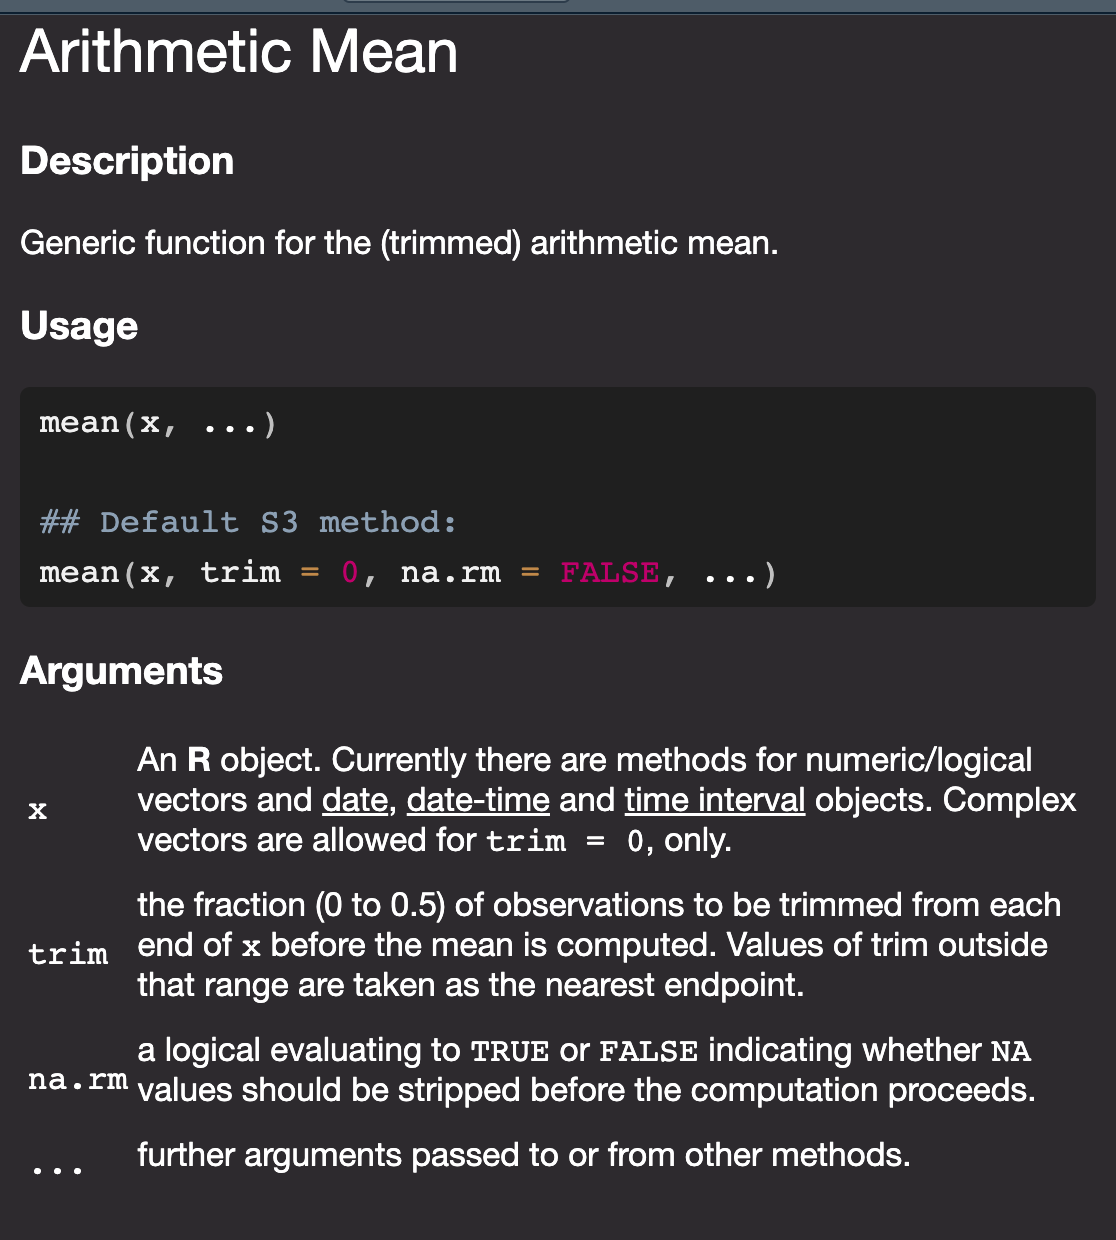
\includegraphics[width=3.72in,height=\textheight]{figs/mean-help.png}

If you look at the help documentation you may see an argument that says
\texttt{na.rm\ =\ FALSE} that is telling mean how to handle missing
values. \texttt{na.rm\ =\ FALSE} in regular human speak just reads as
don't remove missing values. So to get the numbers we wanted all we need
to do is switch the \texttt{na.rm\ =\ FALSE} to \texttt{na.rm\ =\ TRUE}

\begin{Shaded}
\begin{Highlighting}[]
\FunctionTok{mean}\NormalTok{(our\_data}\SpecialCharTok{$}\NormalTok{values, }\AttributeTok{na.rm =} \ConstantTok{TRUE}\NormalTok{)}
\end{Highlighting}
\end{Shaded}

\begin{verbatim}
[1] 3
\end{verbatim}

\marginnote{\begin{footnotesize}

If you do more complex mathy things like \texttt{lm} it will just delete
the missing values which is not always great

\end{footnotesize}}

\hypertarget{loading-and-installing-packages}{%
\section{Loading and installing
packages}\label{loading-and-installing-packages}}

When you first open \texttt{Rstudio} you have some preloaded packages
like \texttt{mean}. However, I will guarantee that when you start
working with \texttt{R} more and you need to do more complex things you
will have to use other functions. The \texttt{tidyverse} is not one of
these packages that is loaded when you open \texttt{Rstudio} so copying
and pasting the code from the knitted document will not work. That is
because \texttt{R} does not have the instructions it needs to run those
commands. To do this you have to download the package. Like with
everything in \texttt{R} there are like a bajillion ways to do this. The
first one is by using the packages window

\includegraphics{pics/install.gif}

Here you just type in the name of the package and then click install.
All that is doing is just running this code

\begin{Shaded}
\begin{Highlighting}[]
\FunctionTok{install.packages}\NormalTok{(}\StringTok{"ggplot2"}\NormalTok{)}
\end{Highlighting}
\end{Shaded}

If you want to install multiple packages what you can do is something
like this.

\begin{Shaded}
\begin{Highlighting}[]
\FunctionTok{install.packages}\NormalTok{(}\FunctionTok{c}\NormalTok{(}\StringTok{"ggplot2"}\NormalTok{, }\StringTok{"palmerpenguins"}\NormalTok{, }\StringTok{"MetBrewer"}\NormalTok{))}
\end{Highlighting}
\end{Shaded}

Remember how earlier I taught you how to define a vector? Well that is
all we are doing here.

Once you install the packages you will not need to reinstall the package
each time. However, these packages are just installed and not loaded.
Unlike excel or other analysis software you have to explicitly tell
\texttt{R} that you want to use a package. The way we do this is by
\texttt{library(packagename)} like this

\begin{Shaded}
\begin{Highlighting}[]
\FunctionTok{library}\NormalTok{(tidyverse)}
\end{Highlighting}
\end{Shaded}

You should always load the packages at the top of your script or quarto
document. \texttt{R} executes things sequentially meaning it starts from
line one and ends once it gets to the bottom of the script or there is
an error.

\begin{Shaded}
\begin{Highlighting}[]
\FunctionTok{library}\NormalTok{(palmerpenguins) }\CommentTok{\# loads in the palmerpenguins data}


\FunctionTok{ggplot}\NormalTok{(penguins, }\FunctionTok{aes}\NormalTok{(}\AttributeTok{x =}\NormalTok{ body\_mass\_g)) }\SpecialCharTok{+}
\FunctionTok{geom\_histogram}\NormalTok{()}
\end{Highlighting}
\end{Shaded}

\begin{verbatim}
Error in ggplot(penguins, aes(x = body_mass_g)): could not find function "ggplot"
\end{verbatim}

\begin{Shaded}
\begin{Highlighting}[]
\FunctionTok{library}\NormalTok{(ggplot2)}

\FunctionTok{ggplot}\NormalTok{(penguins, }\FunctionTok{aes}\NormalTok{(}\AttributeTok{x =}\NormalTok{ body\_mass\_g)) }\SpecialCharTok{+}
\FunctionTok{geom\_histogram}\NormalTok{()}
\end{Highlighting}
\end{Shaded}

\begin{figure}[H]

{\centering 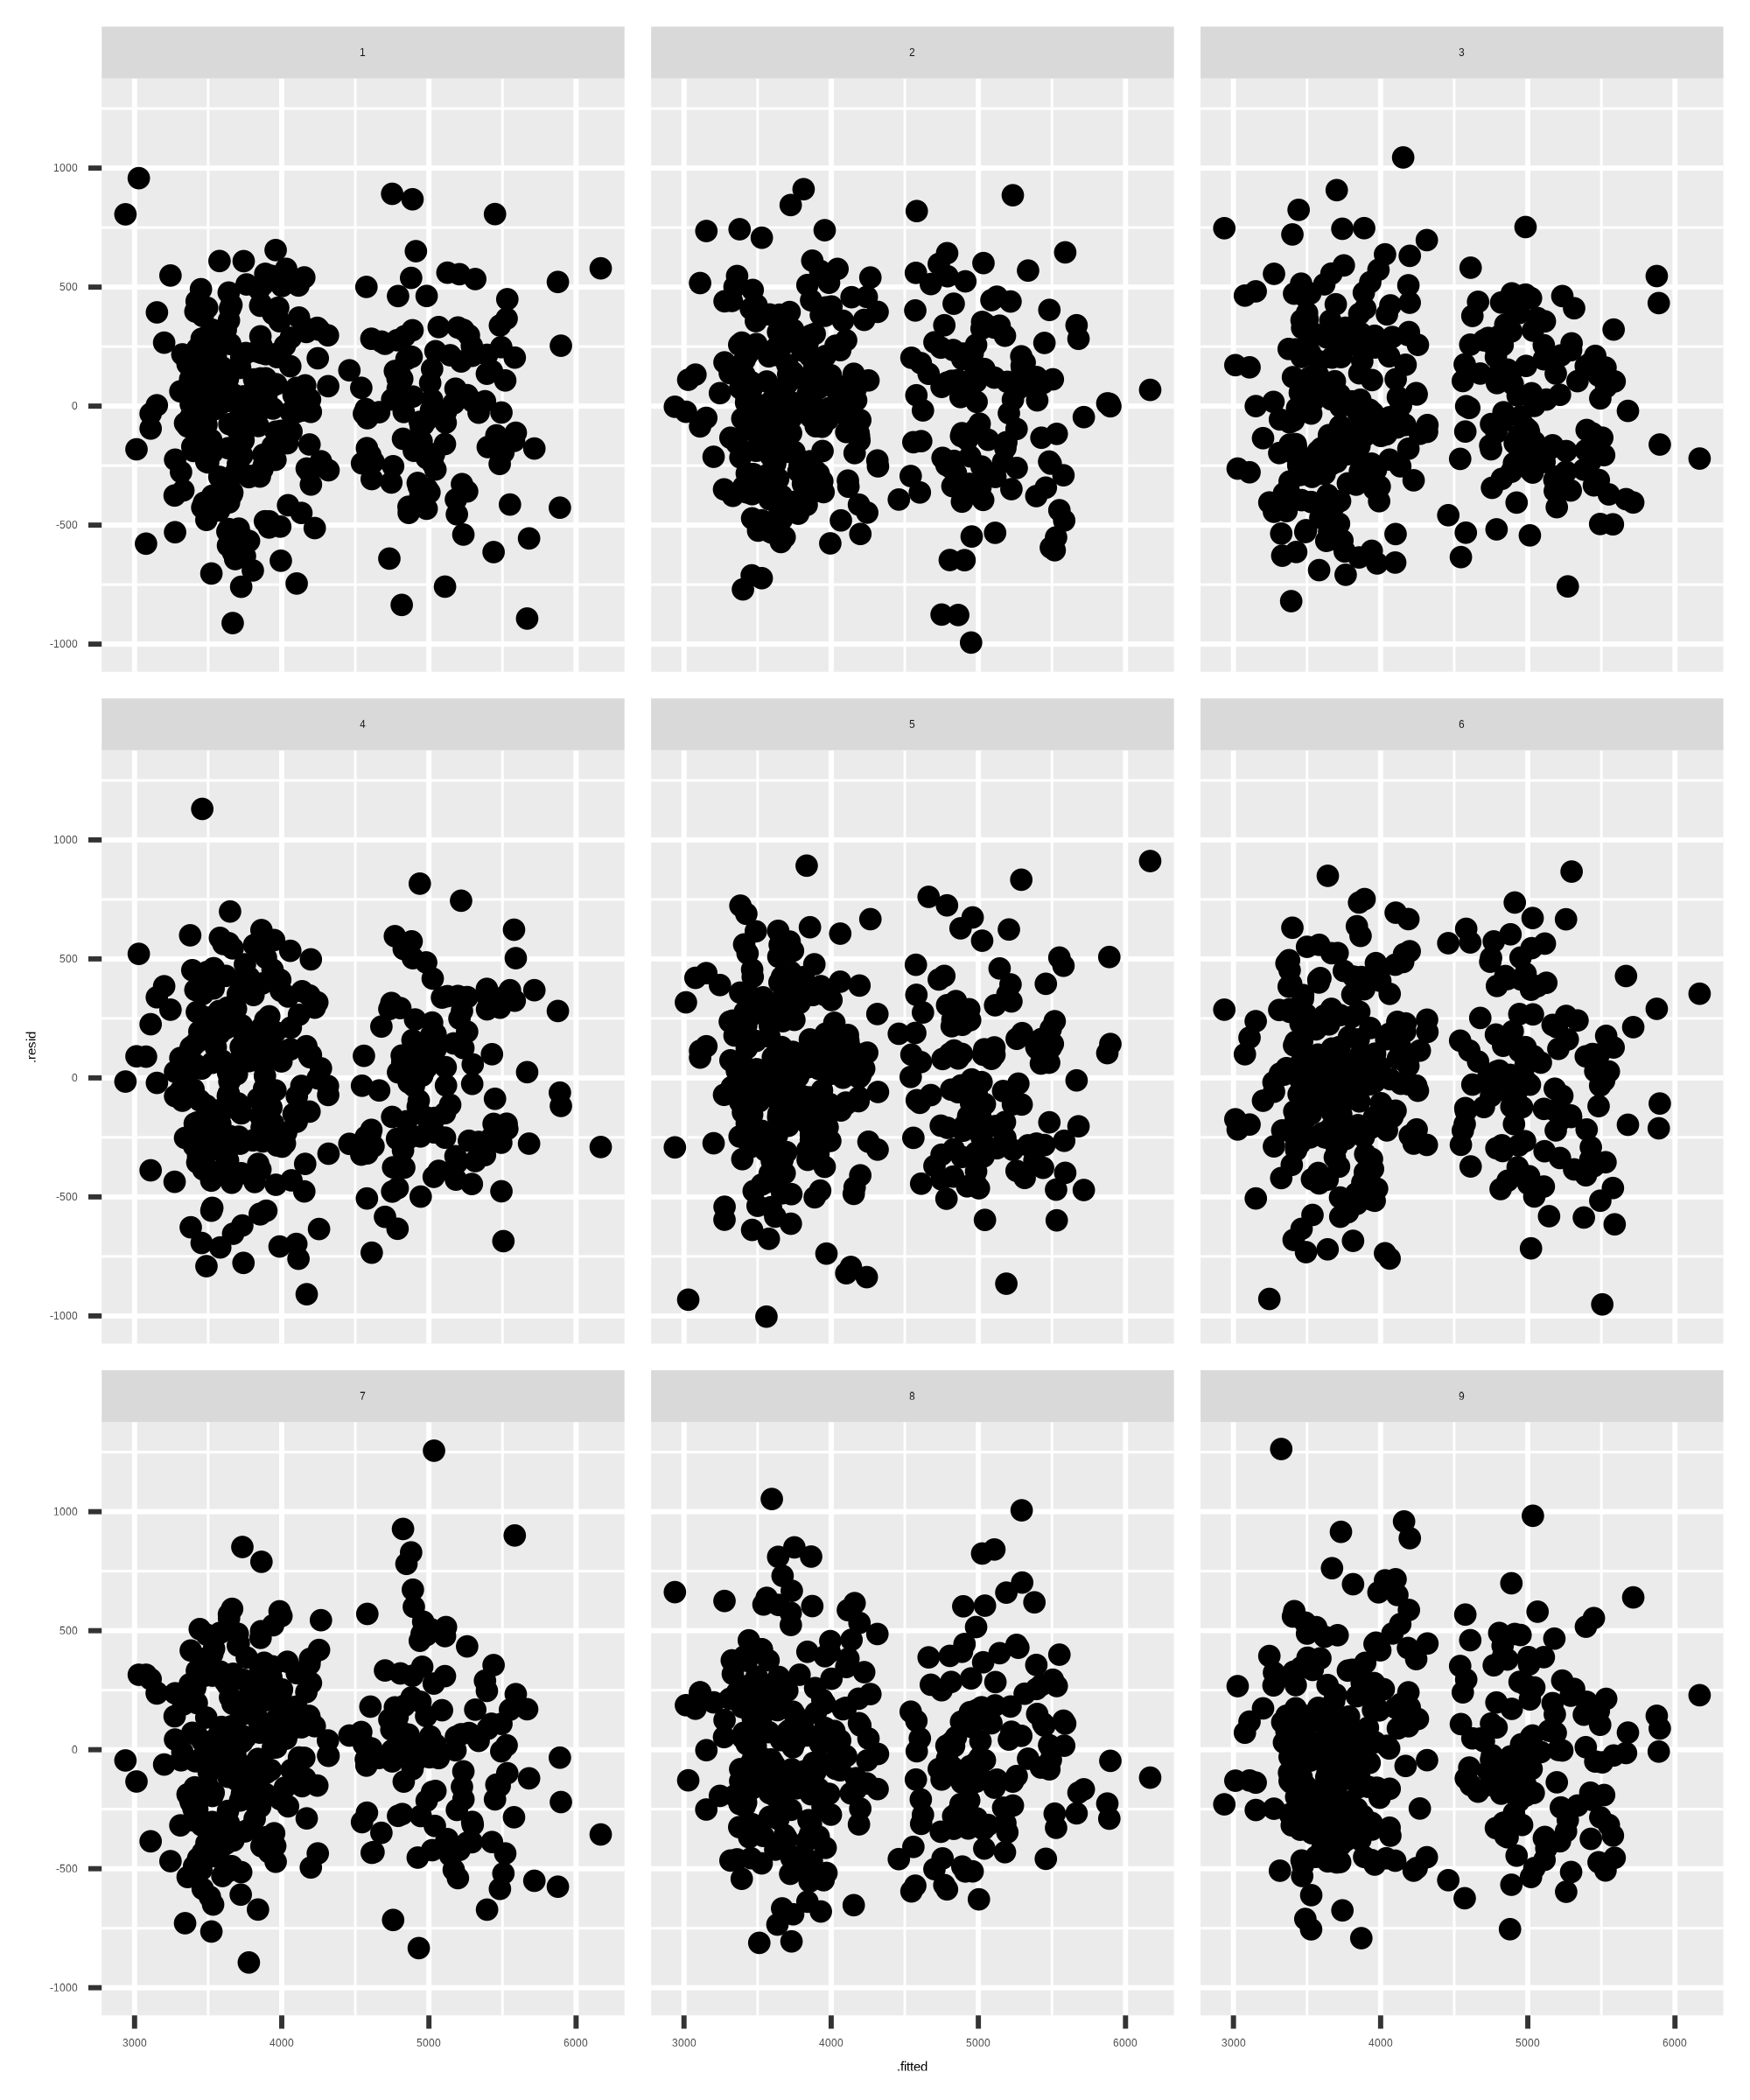
\includegraphics{02-r-basics_files/figure-pdf/unnamed-chunk-42-1.pdf}

}

\end{figure}

Notice how the first set of code generates an error while the second set
of code does not. This is because in the \texttt{library(ggplot2)} line
we have told \texttt{R} to load in the \texttt{ggplot} instructions.

\marginnote{\begin{footnotesize}

One thing you will notice is that once you install the package you do
not need to put the package name in quotation marks. The reason why is
due to the fact that \texttt{R} now recognizes the package as defined
objects with given names.

\end{footnotesize}}

A standard \texttt{R} script/quarto document will have the instructions
loaded at the top like this.

\begin{Shaded}
\begin{Highlighting}[]
\FunctionTok{library}\NormalTok{(ggplot2)}
\FunctionTok{library}\NormalTok{(palmerpenguins)}
\FunctionTok{library}\NormalTok{(MetBrewer)}
\end{Highlighting}
\end{Shaded}

One of the nice things about Rstudio is if you open somebody else's
\texttt{R} script or \texttt{quarto} document and they do something like
\texttt{library(packageIdonthave)} Rstudio will ask if you want to
install it.

\bookmarksetup{startatroot}

\hypertarget{writing-in-quarto}{%
\chapter{Writing in Quarto}\label{writing-in-quarto}}

We have covered what Quarto is, but not how we use it. Quarto is a
really great tool because it lets you combine words and code together.
It relies on something called markdown and pandoc to generate multiple
formats. The details are
\href{https://quarto.org/docs/faq/rmarkdown.html}{covered more
extensively across the internet but this link does a really good job
distilling what goes on}. What is incredibly infuriating about Quarto
from a new user standpoint boils down to (in my experience) a few
things:

\begin{itemize}
\item
  A new syntax to write in
\item
  Not rendering
\item
  Things not being where you think they should be
\end{itemize}

These are all fixable problems as long as we know what could be going
on. For the most part as social scientists we want our documents in one
of two formats either word or pdf. In this section we will mostly deal
with pdf.

\hypertarget{how-to-get-a-pdf}{%
\section{How to Get a PDF}\label{how-to-get-a-pdf}}

\hypertarget{installing-quarto}{%
\subsection{Installing Quarto}\label{installing-quarto}}

The process is relatively straight forward. Just go to
\href{https://quarto.org/docs/get-started/}{the Quarto website} and
click on the download button. This will install Quarto onto your machine
so that is relatively straight forward!

To produce pdfs Quarto relies on something called \(\LaTeX\). All you
really need to know about \(\LaTeX\) is that you need it to produce a
PDF. To install LaTeX all you need to do is open an R script and copy
and paste this code and run it and then type Y and hit enter.

\begin{Shaded}
\begin{Highlighting}[]
\NormalTok{rstudioapi}\SpecialCharTok{::}\FunctionTok{terminalExecute}\NormalTok{(}
  \AttributeTok{command =} \StringTok{"quarto install tinytex"}
\NormalTok{)}
\end{Highlighting}
\end{Shaded}

It may prompt you to enter your password. This is just the password you
use to log into your computer. Nothing will appear when you enter your
password but your password is being entered. The reason your computer
does this is for the same reason that websites do not display your
password. This is installing a very minimal
\href{https://yihui.org/tinytex/}{LaTeX distribution}. After that is
done you can now render PDFs.

Do get the output we want we need to do some stuff in order to tell
quarto what type of document we want. You add this information at the
top of the document like you would with word. However, it looks a little
bit different since it relies on YAML(Yet Another Markdown Language) to
add in this info.\footnote{Yes this is really what it is called. Some
  sites use TOML which is an acronym for Tom's Obvious, Minimal
  Language. Much like political scientists once a joke in a title gets
  started it is doomed to be repeated.} Your YAML heading should look
like this

\begin{Shaded}
\begin{Highlighting}[]
\FunctionTok{title}\KeywordTok{:}\AttributeTok{ }\StringTok{"Quarto Guide"}
\FunctionTok{author}\KeywordTok{:}\AttributeTok{ }\StringTok{"Josh Allen"}
\FunctionTok{date}\KeywordTok{:}\AttributeTok{  }\StringTok{"08/16/23"}
\FunctionTok{format}\KeywordTok{:}\AttributeTok{ pdf}
\end{Highlighting}
\end{Shaded}

From there you can pass additional options to it like what the citation
style, the citation engine, the kind of font you want to use etc. So it
looks something like this.

\begin{Shaded}
\begin{Highlighting}[]
\FunctionTok{title}\KeywordTok{:}\AttributeTok{ }\StringTok{"Quarto Guide"}
\FunctionTok{author}\KeywordTok{:}\AttributeTok{ }\StringTok{"Josh Allen"}
\FunctionTok{date}\KeywordTok{:}\CommentTok{ \# "08/16/23" \# this is to show you how to add the current date}
\FunctionTok{format}\KeywordTok{:}
\AttributeTok{  }\FunctionTok{pdf}\KeywordTok{:}
\AttributeTok{    }\FunctionTok{toc}\KeywordTok{:}\AttributeTok{ }\CharTok{false}\CommentTok{ \# this turns off the table of contents}
\AttributeTok{    }\FunctionTok{mainfont}\KeywordTok{:}\AttributeTok{ }\StringTok{"Cochineal"}\CommentTok{ \# the font I like}
\AttributeTok{    }\FunctionTok{mainfontoptions}\KeywordTok{:}\AttributeTok{ }
\AttributeTok{      }\KeywordTok{{-}}\AttributeTok{ }\StringTok{"Numbers=Proportional"}
\AttributeTok{      }\KeywordTok{{-}}\AttributeTok{ }\StringTok{"Numbers=OldStyle"}
\AttributeTok{    }\FunctionTok{mathfont}\KeywordTok{:}\AttributeTok{ }\StringTok{"Libertinus Math"}
\AttributeTok{    }\FunctionTok{indent}\KeywordTok{:}\AttributeTok{ }\CharTok{true}
\AttributeTok{    }\FunctionTok{geometry}\KeywordTok{:}\AttributeTok{ margin=1in}\CommentTok{ \# one inch margins }
\AttributeTok{    }\FunctionTok{biblio{-}title}\KeywordTok{:}\AttributeTok{ }\StringTok{"References"}
\AttributeTok{    }\FunctionTok{cite{-}method}\KeywordTok{:}\AttributeTok{ biblatex}
\FunctionTok{fontsize}\KeywordTok{:}\AttributeTok{ 12pt}
\FunctionTok{bibliography}\KeywordTok{:}\AttributeTok{ ref.bib}\CommentTok{ \# specify the bib file }
\FunctionTok{biblio{-}style}\KeywordTok{:}\AttributeTok{ apsr}\CommentTok{ \# what style to choose }
\end{Highlighting}
\end{Shaded}

\hypertarget{using-quarto-to-write}{%
\section{Using Quarto to write}\label{using-quarto-to-write}}

If you work in the visual editor than lots of the stuff will be
abstracted away. It should look somewhat familiar to a word

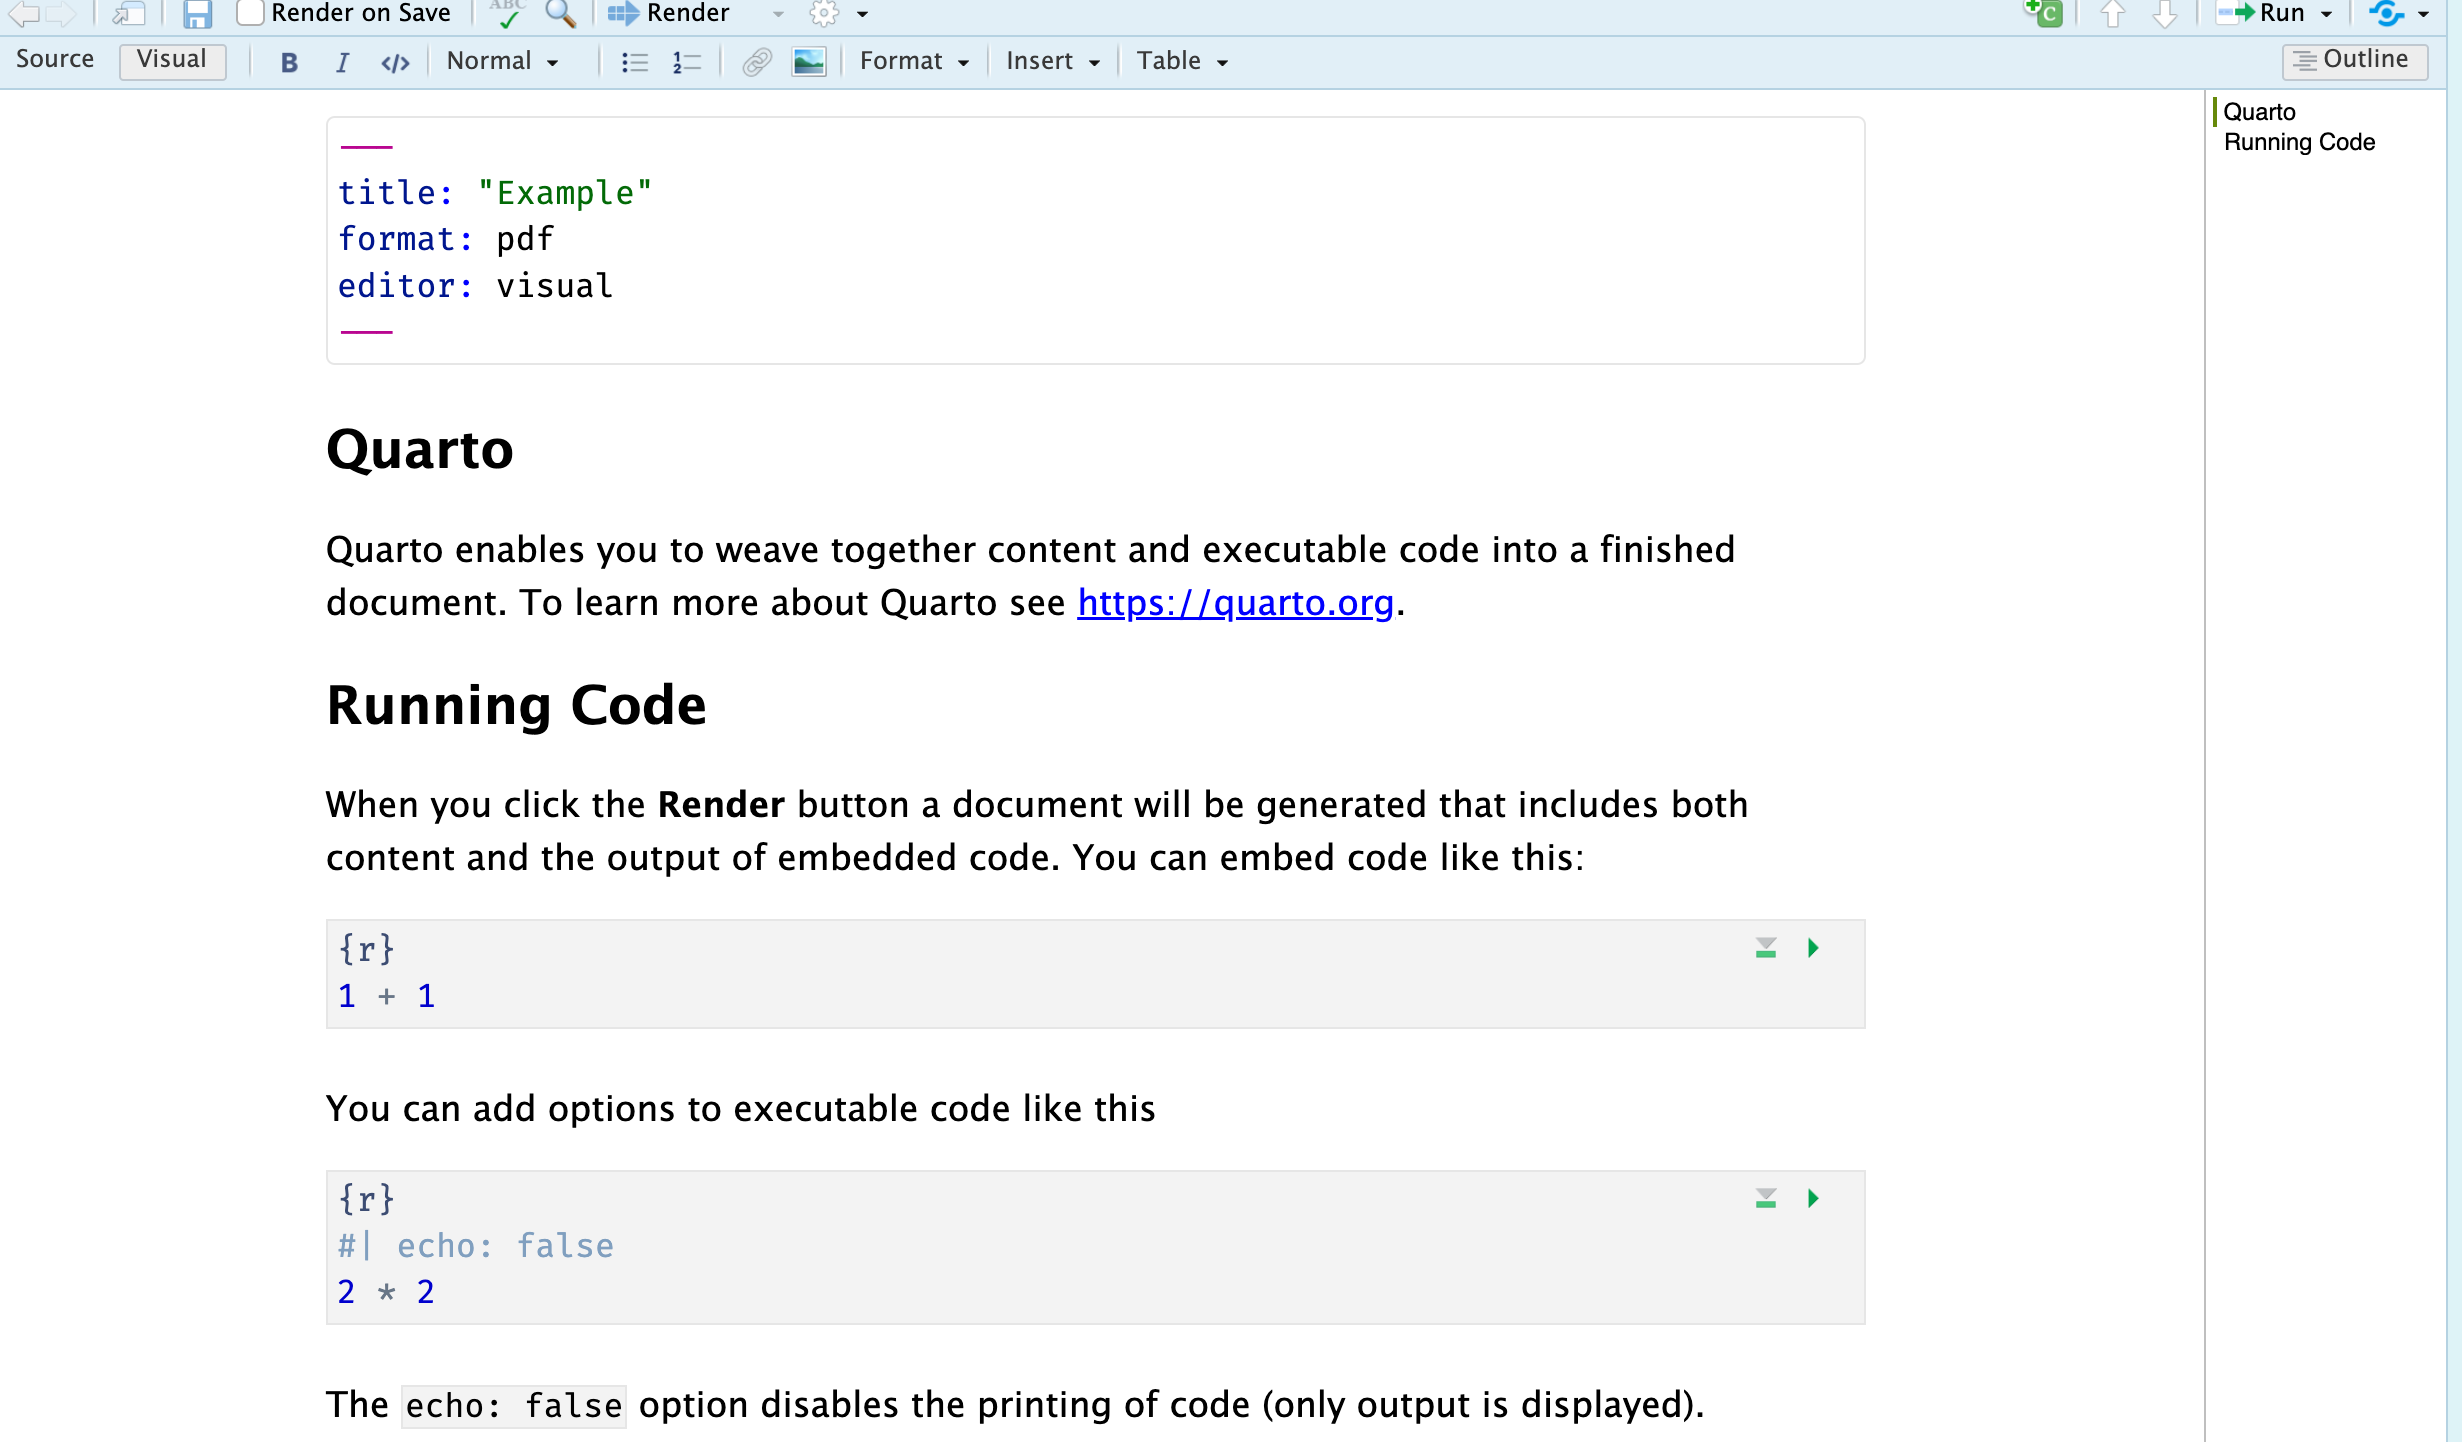
\includegraphics[width=8.21in,height=\textheight]{figs/visual-default.png}

Lot of the same keyboard shortcuts should work! What changes is now you
can insert executable code. The quickest way to do this is by doing
\texttt{cmd\ +\ alt/option\ +\ I} on mac or
\texttt{ctrl\ +\ alt/option\ +\ I} on a windows.

\hypertarget{working-with-the-source-editor}{%
\subsection{Working with the Source
Editor}\label{working-with-the-source-editor}}

Personally I do not really like working with the visual editor which may
just be because I started using \texttt{Rmarkdown} when the visual
editor was not very good. One thing to know is that you will have to
learn some new syntax to write which is fine and you will eventually get
the hang of it.

\hypertarget{writing-in-line}{%
\subsection{Writing in line}\label{writing-in-line}}

Often times we use \emph{italics}, \textbf{bold}, or a mix of
\textbf{\emph{both}} to emphasize things. In word we would either click
the button or in LaTex we would do
\texttt{\textbackslash{}textbf\{something\ like\ this\}}. If you have
learned LaTeX you can still do \(\textbf{this}\) but you would need to
wrap it in dollar signs \texttt{\$\textbackslash{}textbf\{\}\$}. Instead
of doing all that what you can do is just take advantage of markdown
syntax. In the table we can see how to do this

\begin{longtable}[]{@{}
  >{\raggedright\arraybackslash}p{(\columnwidth - 4\tabcolsep) * \real{0.5000}}
  >{\raggedright\arraybackslash}p{(\columnwidth - 4\tabcolsep) * \real{0.4444}}
  >{\raggedright\arraybackslash}p{(\columnwidth - 4\tabcolsep) * \real{0.0139}}@{}}
\toprule\noalign{}
\begin{minipage}[b]{\linewidth}\raggedright
Markdown Syntax
\end{minipage} & \begin{minipage}[b]{\linewidth}\raggedright
Output
\end{minipage} & \begin{minipage}[b]{\linewidth}\raggedright
\end{minipage} \\
\midrule\noalign{}
\endhead
\bottomrule\noalign{}
\endlastfoot
\begin{minipage}[t]{\linewidth}\raggedright
\begin{verbatim}
*italics* and **bold**
\end{verbatim}
\end{minipage} & \emph{italics} and \textbf{bold} & \\
\texttt{\$superscript\^{}2\$\ /\ \$subscript\_2\$} &
\multicolumn{2}{>{\raggedright\arraybackslash}p{(\columnwidth - 4\tabcolsep) * \real{0.4583} + 2\tabcolsep}@{}}{%
\(superscript^2\) / \(subscript_2\)} \\
\begin{minipage}[t]{\linewidth}\raggedright
\begin{verbatim}
~~strikethrough~~
\end{verbatim}
\end{minipage} & \st{strikethrough} & \\
\begin{minipage}[t]{\linewidth}\raggedright
\begin{verbatim}
`verbatim code`
\end{verbatim}
\end{minipage} & \texttt{verbatim\ code} & \\
\end{longtable}

I have yet to come up with a good mneumonic device on how to remember
the difference between italics and bold. Maybe some day.

\hypertarget{code-and-chunk-options}{%
\subsection{Code and Chunk options}\label{code-and-chunk-options}}

What differentiates Quarto from Word is the ability to embed code
alongside words. To control how these appear in your document you need
to add certain options to your code chunks. The most common thing you
will want to do is stop the code from appearing in documents. For your
problem sets or presenting to a more technical audience you will want to
do this. We can do control that via \texttt{echo}. If we want people to
see our code than we do \texttt{\#\textbar{}\ echo:\ true} like this

\begin{Shaded}
\begin{Highlighting}[]
\InformationTok{\textasciigrave{}\textasciigrave{}\textasciigrave{}\{r show{-}code\}}

\CommentTok{\#| echo: true }
\FunctionTok{library}\NormalTok{(palmerpenguins)}
\FunctionTok{library}\NormalTok{(ggplot2)}

\FunctionTok{ggplot}\NormalTok{(penguins, }\FunctionTok{aes}\NormalTok{(}\AttributeTok{x =}\NormalTok{ body\_mass\_g)) }\SpecialCharTok{+}
\FunctionTok{geom\_histogram}\NormalTok{()}
\InformationTok{\textasciigrave{}\textasciigrave{}\textasciigrave{}}
\end{Highlighting}
\end{Shaded}

which produces

\begin{Shaded}
\begin{Highlighting}[]
\FunctionTok{library}\NormalTok{(palmerpenguins)}
\FunctionTok{library}\NormalTok{(ggplot2)}

\FunctionTok{ggplot}\NormalTok{(penguins, }\FunctionTok{aes}\NormalTok{(}\AttributeTok{x =}\NormalTok{ body\_mass\_g)) }\SpecialCharTok{+}
\FunctionTok{geom\_histogram}\NormalTok{()}
\end{Highlighting}
\end{Shaded}

\begin{verbatim}
`stat_bin()` using `bins = 30`. Pick better value with `binwidth`.
\end{verbatim}

\begin{verbatim}
Warning: Removed 2 rows containing non-finite values (`stat_bin()`).
\end{verbatim}

\begin{figure}[H]

{\centering 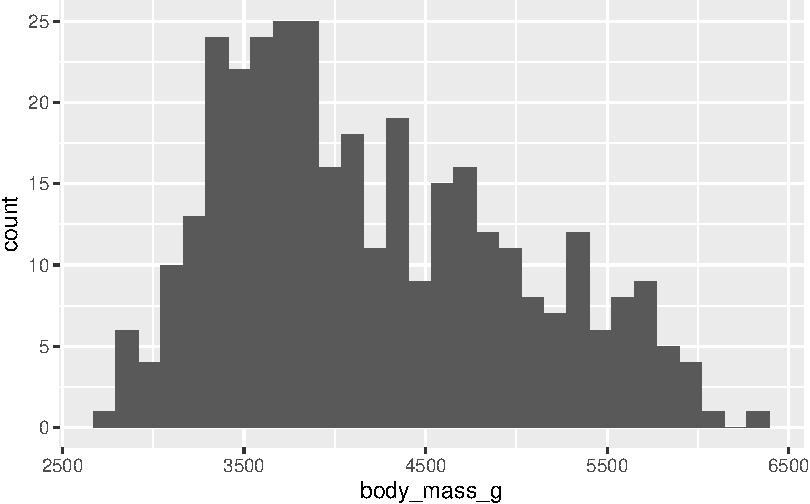
\includegraphics{quarto-basics_files/figure-pdf/unnamed-chunk-3-1.pdf}

}

\end{figure}

If we do not want to show our code than we just do \#\textbar{} echo:
false`

\begin{Shaded}
\begin{Highlighting}[]
\InformationTok{\textasciigrave{}\textasciigrave{}\textasciigrave{}\{r show{-}code\}}

\CommentTok{\#| echo: false }
\FunctionTok{library}\NormalTok{(palmerpenguins)}
\FunctionTok{library}\NormalTok{(ggplot2)}

\FunctionTok{ggplot}\NormalTok{(penguins, }\FunctionTok{aes}\NormalTok{(}\AttributeTok{x =}\NormalTok{ body\_mass\_g)) }\SpecialCharTok{+}
\FunctionTok{geom\_histogram}\NormalTok{()}
\InformationTok{\textasciigrave{}\textasciigrave{}\textasciigrave{}}
\end{Highlighting}
\end{Shaded}

which produces

\begin{verbatim}
`stat_bin()` using `bins = 30`. Pick better value with `binwidth`.
\end{verbatim}

\begin{verbatim}
Warning: Removed 2 rows containing non-finite values (`stat_bin()`).
\end{verbatim}

\includegraphics{quarto-basics_files/figure-pdf/unnamed-chunk-4-1.pdf}

Notice how \texttt{ggplot} is warning us about the bin width we choose.
To control this we just have to change our chunk options by adding
\texttt{\#\textbar{}\ warning:\ false}

\begin{Shaded}
\begin{Highlighting}[]
\InformationTok{\textasciigrave{}\textasciigrave{}\textasciigrave{}\{r warning{-}example\}}

\CommentTok{\#| echo: false }
\CommentTok{\#| warning: false}
\FunctionTok{library}\NormalTok{(palmerpenguins)}
\FunctionTok{library}\NormalTok{(ggplot2)}

\FunctionTok{ggplot}\NormalTok{(penguins, }\FunctionTok{aes}\NormalTok{(}\AttributeTok{x =}\NormalTok{ body\_mass\_g)) }\SpecialCharTok{+}
\FunctionTok{geom\_histogram}\NormalTok{()}
\InformationTok{\textasciigrave{}\textasciigrave{}\textasciigrave{}}
\end{Highlighting}
\end{Shaded}

which produces

\includegraphics{quarto-basics_files/figure-pdf/unnamed-chunk-5-1.pdf}

Similarly if we load in the tidyverse or a package with names of
similarly named functions we will get warnings and messages like this

\begin{Shaded}
\begin{Highlighting}[]
\FunctionTok{library}\NormalTok{(tidyverse)}
\end{Highlighting}
\end{Shaded}

\begin{verbatim}
-- Attaching core tidyverse packages ------------------------ tidyverse 2.0.0 --
v dplyr     1.1.2     v readr     2.1.4
v forcats   1.0.0     v stringr   1.5.0
v lubridate 1.9.2     v tibble    3.2.1
v purrr     1.0.2     v tidyr     1.3.0
-- Conflicts ------------------------------------------ tidyverse_conflicts() --
x dplyr::filter() masks stats::filter()
x dplyr::lag()    masks stats::lag()
i Use the conflicted package (<http://conflicted.r-lib.org/>) to force all conflicts to become errors
\end{verbatim}

Again all we need to do to omit this is just change the chunk options

\begin{Shaded}
\begin{Highlighting}[]
\InformationTok{\textasciigrave{}\textasciigrave{}\textasciigrave{}\{r message{-}example\}}
\CommentTok{\#| message: false}

\FunctionTok{library}\NormalTok{(tidyverse)}

\InformationTok{\textasciigrave{}\textasciigrave{}\textasciigrave{}}
\end{Highlighting}
\end{Shaded}

which produces

\begin{Shaded}
\begin{Highlighting}[]
\FunctionTok{library}\NormalTok{(tidyverse)}
\end{Highlighting}
\end{Shaded}

Notice how there is no big long warning message. One other thing to
notice is that I have named the code chunks like
\texttt{message-example}. This is good practice because it makes hoping
around the document a little bit easier. Because it will say failed
something to the effect of
\texttt{quitting\ on\ line\ 12-20\ code-for-fig-1}. Which will let you
navigate there a bit easier.

\part{Doing Stuff With Data}

\bookmarksetup{startatroot}

\hypertarget{intro-to-the-tidyverse}{%
\chapter{Intro to the tidyverse}\label{intro-to-the-tidyverse}}

As an
\href{https://en.wikipedia.org/wiki/Object-oriented_programming}{object
oriented programming language (OOP)}, R is not particularly
user-friendly and thus
\href{https://www.tidyverse.org/}{\texttt{\{tidyverse\}}}--a suite of
data management, \href{https://ggplot2.tidyverse.org/}{visualization},
and \href{https://www.tidymodels.org/}{modeling} packages--aims to turn
R into \href{https://tidyverse.tidyverse.org/articles/manifesto.html}{a
more user-friendly functional programming language}. As one of the
project's major developers, Hadley Wickham, recently put it ``R is not a
language driven by the purity of its philosophy; R is a language
designed to get shit done.'' This may have become some what evident in
the indexing section where I talked about \texttt{{[}{]}},
\texttt{{[}{[}{]}{]}}, and \texttt{\$}. In general languages like Python
only have one way to index an object.

The tidyverse is actually a collection of packages that share the same
underlying philosophy (which we will get to). Generally I will load in
the tidyverse like this.

\begin{Shaded}
\begin{Highlighting}[]
\FunctionTok{library}\NormalTok{(tidyverse)}
\end{Highlighting}
\end{Shaded}

\begin{verbatim}
-- Attaching core tidyverse packages ------------------------ tidyverse 2.0.0 --
v dplyr     1.1.2     v readr     2.1.4
v forcats   1.0.0     v stringr   1.5.0
v ggplot2   3.4.3     v tibble    3.2.1
v lubridate 1.9.2     v tidyr     1.3.0
v purrr     1.0.2     
-- Conflicts ------------------------------------------ tidyverse_conflicts() --
x dplyr::filter() masks stats::filter()
x dplyr::lag()    masks stats::lag()
i Use the conflicted package (<http://conflicted.r-lib.org/>) to force all conflicts to become errors
\end{verbatim}

\hypertarget{dplyr}{%
\section{\texorpdfstring{\texttt{dplyr}}{dplyr}}\label{dplyr}}

\begin{tcolorbox}[enhanced jigsaw, breakable, colback=white, left=2mm, bottomrule=.15mm, opacityback=0, toprule=.15mm, arc=.35mm, rightrule=.15mm, leftrule=.75mm]

``Happy families are all alike; every unhappy family is unhappy in its
own way.'' - Leon Tolstoy.

\end{tcolorbox}

Data is often talked about the in the same way. All clean datasets are
alike in structure and dignity. Every messy dataset is messy in its own
special way.

\texttt{dplyr} is the tidyverse way to manipulate data and an all around
great package. But you need to get the basic functions right. Cleaning
data is what you will spend the most time on.

We will use the \texttt{palmerpenguins} and the starwars dataset to
demonstrate how to use the \texttt{verbs} in \texttt{dplyr}

\begin{Shaded}
\begin{Highlighting}[]
\FunctionTok{data}\NormalTok{(}\StringTok{"starwars"}\NormalTok{)}
\FunctionTok{library}\NormalTok{(palmerpenguins)}
\end{Highlighting}
\end{Shaded}

\hypertarget{select}{%
\subsection{\texorpdfstring{\texttt{select}}{select}}\label{select}}

Select is the most intuitive. Select picks out the columns you want or,
in some cases, do not want. If we only want the name of the character
and the place they are from we feed that name of the columns into
select. If you are following along and copying and pasting the code in
the guide to see what is going on you may notice that your output
differs slightly. That is because behind the scenes I am just using
select to cut down on the output.

\begin{Shaded}
\begin{Highlighting}[]
\FunctionTok{select}\NormalTok{(starwars, name, homeworld)}
\end{Highlighting}
\end{Shaded}

\begin{tabular}{l|l}
\hline
name & homeworld\\
\hline
Luke Skywalker & Tatooine\\
\hline
C-3PO & Tatooine\\
\hline
R2-D2 & Naboo\\
\hline
Darth Vader & Tatooine\\
\hline
Leia Organa & Alderaan\\
\hline
\end{tabular}

If we wanted all the columns \textbf{except} for name and homeworld we
would do this.

\begin{Shaded}
\begin{Highlighting}[]
\FunctionTok{select}\NormalTok{(starwars, }\SpecialCharTok{{-}}\NormalTok{name, }\SpecialCharTok{{-}}\NormalTok{homeworld)}
\end{Highlighting}
\end{Shaded}

\begin{tabular}{r|r|l|l|l|l}
\hline
height & mass & hair\_color & skin\_color & eye\_color & starships\\
\hline
172 & 77 & blond & fair & blue & X-wing          , Imperial shuttle\\
\hline
167 & 75 & NA & gold & yellow & \\
\hline
96 & 32 & NA & white, blue & red & \\
\hline
202 & 136 & none & white & yellow & TIE Advanced x1\\
\hline
150 & 49 & brown & light & brown & \\
\hline
\end{tabular}

We can also feed it a range of columns using \texttt{:}

\begin{Shaded}
\begin{Highlighting}[]
\FunctionTok{select}\NormalTok{(starwars, name}\SpecialCharTok{:}\NormalTok{hair\_color)}
\end{Highlighting}
\end{Shaded}

\begin{tabular}{l|r|r|l}
\hline
name & height & mass & hair\_color\\
\hline
Luke Skywalker & 172 & 77 & blond\\
\hline
C-3PO & 167 & 75 & NA\\
\hline
R2-D2 & 96 & 32 & NA\\
\hline
Darth Vader & 202 & 136 & none\\
\hline
Leia Organa & 150 & 49 & brown\\
\hline
\end{tabular}

\hypertarget{filter}{%
\subsection{\texorpdfstring{\texttt{filter}}{filter}}\label{filter}}

Filter is how we subset by rows. To do this we need to tell filter what
rows we want! This feels like it should be intuitive, but we have to use
some concepts that are likely new to you. Lets say we want characters
that are from a particular world in starwars. To do that we do this.

\begin{Shaded}
\begin{Highlighting}[]
\FunctionTok{filter}\NormalTok{(starwars, homeworld }\SpecialCharTok{==} \StringTok{"Naboo"}\NormalTok{) }
\end{Highlighting}
\end{Shaded}

\begin{tabular}{l|l}
\hline
name & homeworld\\
\hline
R2-D2 & Naboo\\
\hline
Palpatine & Naboo\\
\hline
Jar Jar Binks & Naboo\\
\hline
Roos Tarpals & Naboo\\
\hline
Rugor Nass & Naboo\\
\hline
\end{tabular}

What we are doing here is just creating a dataset with just things from
Naboo. We need to set tell \texttt{R} what rows we want by setting up
some tests. Each time a row meets that condition then \texttt{R} is
going to grab it. As a reminder these are the kinds of test you can do

Test

Meaning

Test

Meaning

x \textless{} y

Less than

x \%in\% y

In set

x \textgreater{} y

Greater than

is.na(x)

Is missing

==

Equal to

!is.na(x)

Is not missing

x \textless= y

Less than or equal to

! y

Not

x \textgreater= y

Greater than or equal to

x != y

Not equal to

x \textbar{} y

Or

x \& y

And

So lets return back to our Naboo example. If we wanted to reuse this
dataset later we would assign it to an object using
\texttt{\textless{}-} so lets assign it to an object named
\texttt{naboo}

\begin{Shaded}
\begin{Highlighting}[]
\NormalTok{naboo }\OtherTok{\textless{}{-}} \FunctionTok{filter}\NormalTok{(starwars, homeworld }\SpecialCharTok{==} \StringTok{"Naboo"}\NormalTok{) }
\end{Highlighting}
\end{Shaded}

We can also combine multiple tests in filter. Lets say we wanted to all
the characters that are from Naboo and are human

\begin{Shaded}
\begin{Highlighting}[]
 \FunctionTok{filter}\NormalTok{(starwars, homeworld }\SpecialCharTok{==} \StringTok{"Naboo"} \SpecialCharTok{\&}\NormalTok{ species }\SpecialCharTok{==} \StringTok{"Human"}\NormalTok{)}
\end{Highlighting}
\end{Shaded}

\begin{tabular}{l|l|l}
\hline
name & species & homeworld\\
\hline
Palpatine & Human & Naboo\\
\hline
Gregar Typho & Human & Naboo\\
\hline
Cordé & Human & Naboo\\
\hline
Dormé & Human & Naboo\\
\hline
Padmé Amidala & Human & Naboo\\
\hline
\end{tabular}

Now we have all the characters that are from Naboo and are human! Filter
automatically defaults to an and test. So these produce the same
behavior.

\begin{Shaded}
\begin{Highlighting}[]
\FunctionTok{filter}\NormalTok{(starwars, homeworld }\SpecialCharTok{==} \StringTok{"Naboo"} \SpecialCharTok{\&}\NormalTok{ species }\SpecialCharTok{==} \StringTok{"Human"}\NormalTok{) }

\FunctionTok{filter}\NormalTok{(starwars, homeworld }\SpecialCharTok{==} \StringTok{"Naboo"}\NormalTok{, species }\SpecialCharTok{==} \StringTok{"Human"}\NormalTok{)}
\end{Highlighting}
\end{Shaded}

\begin{tabular}{l|l|l}
\hline
name & homeworld & species\\
\hline
Palpatine & Naboo & Human\\
\hline
Gregar Typho & Naboo & Human\\
\hline
Cordé & Naboo & Human\\
\hline
Dormé & Naboo & Human\\
\hline
Padmé Amidala & Naboo & Human\\
\hline
\end{tabular}

\begin{tabular}{l|l|l}
\hline
name & homeworld & species\\
\hline
Palpatine & Naboo & Human\\
\hline
Gregar Typho & Naboo & Human\\
\hline
Cordé & Naboo & Human\\
\hline
Dormé & Naboo & Human\\
\hline
Padmé Amidala & Naboo & Human\\
\hline
\end{tabular}

If we wanted characters from two different homeworlds we would do an or
test using \texttt{\textbar{}} (the key above enter/return)

\begin{Shaded}
\begin{Highlighting}[]
\FunctionTok{filter}\NormalTok{(starwars, homeworld }\SpecialCharTok{==} \StringTok{"Naboo"} \SpecialCharTok{|}\NormalTok{ homeworld }\SpecialCharTok{==} \StringTok{"Tatooine"}\NormalTok{)}
\end{Highlighting}
\end{Shaded}

\begin{tabular}{l|l}
\hline
name & homeworld\\
\hline
Luke Skywalker & Tatooine\\
\hline
C-3PO & Tatooine\\
\hline
R2-D2 & Naboo\\
\hline
Darth Vader & Tatooine\\
\hline
Owen Lars & Tatooine\\
\hline
\end{tabular}

The reason we would use an or test is because one character can't have
two homeworlds! Remember, computers are dumb. As long as the code can
run, it will do it. So if we use an and test, this is what it returns

\begin{Shaded}
\begin{Highlighting}[]
\FunctionTok{filter}\NormalTok{(starwars, homeworld }\SpecialCharTok{==} \StringTok{"Naboo"} \SpecialCharTok{\&}\NormalTok{ homeworld }\SpecialCharTok{==} \StringTok{"Tatooine"}\NormalTok{)}
\end{Highlighting}
\end{Shaded}

\begin{verbatim}
# A tibble: 0 x 14
# i 14 variables: name <chr>, height <int>, mass <dbl>, hair_color <chr>,
#   skin_color <chr>, eye_color <chr>, birth_year <dbl>, sex <chr>,
#   gender <chr>, homeworld <chr>, species <chr>, films <list>,
#   vehicles <list>, starships <list>
\end{verbatim}

When working with things in \texttt{R} stray commas and spelling will
lead to headaches. Here is an example that would not throw an error but
will create a dataframe with zero observations. Naboo exists as a value
of homeworld, but naboo does not.

\begin{Shaded}
\begin{Highlighting}[]
\NormalTok{ naboo }\OtherTok{\textless{}{-}} \FunctionTok{filter}\NormalTok{(starwars, homeworld }\SpecialCharTok{==} \StringTok{"naboo"}\NormalTok{)}

\NormalTok{naboo }\OtherTok{\textless{}{-}} \FunctionTok{filter}\NormalTok{(starwars, homeworld }\SpecialCharTok{==} \StringTok{"Naboo"}\NormalTok{,)}
\end{Highlighting}
\end{Shaded}

Filter also works if you want particular values of something. Let's say
we want penguins with longer flippers or characters less than a certain
height. We can do that with filter.

\begin{Shaded}
\begin{Highlighting}[]
\FunctionTok{filter}\NormalTok{(starwars, height }\SpecialCharTok{\textless{}} \FunctionTok{mean}\NormalTok{(height, }\AttributeTok{na.rm =} \ConstantTok{TRUE}\NormalTok{))}

\FunctionTok{filter}\NormalTok{(penguins, flipper\_length\_mm }\SpecialCharTok{\textgreater{}} \DecValTok{2}\NormalTok{)}
\end{Highlighting}
\end{Shaded}

\begin{tabular}{l|r|l}
\hline
name & height & species\\
\hline
Luke Skywalker & 172 & Human\\
\hline
C-3PO & 167 & Droid\\
\hline
R2-D2 & 96 & Droid\\
\hline
Leia Organa & 150 & Human\\
\hline
Beru Whitesun lars & 165 & Human\\
\hline
\end{tabular}

\begin{tabular}{l|r}
\hline
species & flipper\_length\_mm\\
\hline
Adelie & 181\\
\hline
Adelie & 186\\
\hline
Adelie & 195\\
\hline
Adelie & 193\\
\hline
Adelie & 190\\
\hline
\end{tabular}

Sometimes we want a dataset that does not have any missing values in it
for a particular column. In this case all we do is just add \texttt{!}
in front of the \texttt{is.na} function.

\begin{Shaded}
\begin{Highlighting}[]
\FunctionTok{filter}\NormalTok{(starwars, }\SpecialCharTok{!}\FunctionTok{is.na}\NormalTok{(height))}
\end{Highlighting}
\end{Shaded}

\begin{tabular}{l|r|r|l|l|l}
\hline
name & height & mass & hair\_color & skin\_color & eye\_color\\
\hline
Luke Skywalker & 172 & 77 & blond & fair & blue\\
\hline
C-3PO & 167 & 75 & NA & gold & yellow\\
\hline
R2-D2 & 96 & 32 & NA & white, blue & red\\
\hline
Darth Vader & 202 & 136 & none & white & yellow\\
\hline
Leia Organa & 150 & 49 & brown & light & brown\\
\hline
\end{tabular}

We would do something similar if we wanted characters that are not
human!

\begin{Shaded}
\begin{Highlighting}[]
\FunctionTok{filter}\NormalTok{(starwars, species }\SpecialCharTok{!=} \StringTok{"Human"}\NormalTok{)}
\end{Highlighting}
\end{Shaded}

\begin{tabular}{l|r|r|l|l|l|r|l|l|l|l|l|l|l}
\hline
name & height & mass & hair\_color & skin\_color & eye\_color & birth\_year & sex & gender & homeworld & species & films & vehicles & starships\\
\hline
C-3PO & 167 & 75 & NA & gold & yellow & 112 & none & masculine & Tatooine & Droid & The Empire Strikes Back, Attack of the Clones   , The Phantom Menace     , Revenge of the Sith    , Return of the Jedi     , A New Hope &  & \\
\hline
R2-D2 & 96 & 32 & NA & white, blue & red & 33 & none & masculine & Naboo & Droid & The Empire Strikes Back, Attack of the Clones   , The Phantom Menace     , Revenge of the Sith    , Return of the Jedi     , A New Hope             , The Force Awakens &  & \\
\hline
R5-D4 & 97 & 32 & NA & white, red & red & NA & none & masculine & Tatooine & Droid & A New Hope &  & \\
\hline
Chewbacca & 228 & 112 & brown & unknown & blue & 200 & male & masculine & Kashyyyk & Wookiee & The Empire Strikes Back, Revenge of the Sith    , Return of the Jedi     , A New Hope             , The Force Awakens & AT-ST & Millennium Falcon, Imperial shuttle\\
\hline
Greedo & 173 & 74 & NA & green & black & 44 & male & masculine & Rodia & Rodian & A New Hope &  & \\
\hline
\end{tabular}

One last operator that I will show you is the \texttt{\%in\%} operator.
This comes in really handy for lots of things. Intuitively we can think
about it as a bunch of \texttt{thing\ ==\ "value"}\textbar{} thing ==
``value''` tests glued together. Lets say we wanted all the characters
from Tatooine, Naboo, and ``Coruscant''. With what we know we would do
something like this.

\begin{Shaded}
\begin{Highlighting}[]
\FunctionTok{filter}\NormalTok{(starwars, homeworld }\SpecialCharTok{==} \StringTok{"Naboo"} \SpecialCharTok{|}\NormalTok{ homeworld }\SpecialCharTok{==} \StringTok{"Coruscant"} \SpecialCharTok{|}\NormalTok{ homeworld }\SpecialCharTok{==} \StringTok{"Tatooine"}\NormalTok{)}
\end{Highlighting}
\end{Shaded}

While not the most amount of typing in the world this can quickly get to
be a lot if there is a bunch of mutually exclusive things we need to
subset our data by. This is where the \texttt{\%in\%}operator comes in
to save us! We can rewrite this series of or tests like this

\begin{Shaded}
\begin{Highlighting}[]
\FunctionTok{filter}\NormalTok{(starwars, homeworld }\SpecialCharTok{\%in\%} \FunctionTok{c}\NormalTok{(}\StringTok{"Naboo"}\NormalTok{, }\StringTok{"Coruscant"}\NormalTok{, }\StringTok{"Tatooine"}\NormalTok{))}
\end{Highlighting}
\end{Shaded}

\begin{tabular}{l|l}
\hline
name & homeworld\\
\hline
Luke Skywalker & Tatooine\\
\hline
Anakin Skywalker & Tatooine\\
\hline
Finis Valorum & Coruscant\\
\hline
Shmi Skywalker & Tatooine\\
\hline
Adi Gallia & Coruscant\\
\hline
Jocasta Nu & Coruscant\\
\hline
Padmé Amidala & Naboo\\
\hline
\end{tabular}

\marginnote{\begin{footnotesize}

I have done some additional filtering behind the scenes to show you that
it worked so your dataset likely looks a little different.

\end{footnotesize}}

Notice how the test works. The first thing is the name of the variable
and the second is the stuff the homeworlds. What \texttt{R} is doing is
taking the values of the homeworld variable for each row and seeing if
they match whats on the right hand side of \texttt{\%in}. Kind of like
this

\begin{Shaded}
\begin{Highlighting}[]
\DecValTok{5} \SpecialCharTok{\%in\%} \DecValTok{1}\SpecialCharTok{:}\DecValTok{10}
\end{Highlighting}
\end{Shaded}

\begin{verbatim}
[1] TRUE
\end{verbatim}

If we wanted all things outside of this subset we can do this

\begin{Shaded}
\begin{Highlighting}[]
\FunctionTok{filter}\NormalTok{(starwars, }\SpecialCharTok{!}\NormalTok{homeworld }\SpecialCharTok{\%in\%} \FunctionTok{c}\NormalTok{(}\StringTok{"Naboo"}\NormalTok{, }\StringTok{"Coruscant"}\NormalTok{, }\StringTok{"Tatooine"}\NormalTok{))}
\end{Highlighting}
\end{Shaded}

\begin{tabular}{l|l}
\hline
name & homeworld\\
\hline
Leia Organa & Alderaan\\
\hline
Obi-Wan Kenobi & Stewjon\\
\hline
Wilhuff Tarkin & Eriadu\\
\hline
Chewbacca & Kashyyyk\\
\hline
Han Solo & Corellia\\
\hline
\end{tabular}

\hypertarget{mutate}{%
\subsection{\texorpdfstring{\texttt{mutate}}{mutate}}\label{mutate}}

\texttt{mutate} is how we create new columns in our dataset. There are
tons of things that we may need to do in order to create variables. So
lets start with making what we know as an indicator variable. Lets say
we want to create a variable that indicates whether a character is human
or not. We use the \texttt{ifelse} function to do this. The first thing
we need to do is name the column. Lets call this column human. We then
need to tell \texttt{R} what values the human variable has. If we want
to create an indicator variable we can use the \texttt{ifelse} function
in \texttt{R} which kind of works like \texttt{filter}.

\texttt{ifelse} has a few components

\begin{Shaded}
\begin{Highlighting}[]
\FunctionTok{ifelse}\NormalTok{(test, what it does }\ControlFlowTok{if}\NormalTok{ true, what it does }\ControlFlowTok{if}\NormalTok{ false)}
\end{Highlighting}
\end{Shaded}

So in our case if the species column has a value of ``human'' than it
returns \texttt{TRUE} otherwise return \texttt{FALSE}.

\begin{Shaded}
\begin{Highlighting}[]
\FunctionTok{mutate}\NormalTok{(starwars, }\AttributeTok{human =} \FunctionTok{ifelse}\NormalTok{(species }\SpecialCharTok{==} \StringTok{"Human"}\NormalTok{, }\ConstantTok{TRUE}\NormalTok{, }\ConstantTok{FALSE}\NormalTok{))}
\end{Highlighting}
\end{Shaded}

\begin{tabular}{l|l}
\hline
name & species\\
\hline
Luke Skywalker & Human\\
\hline
C-3PO & Droid\\
\hline
R2-D2 & Droid\\
\hline
Darth Vader & Human\\
\hline
Leia Organa & Human\\
\hline
\end{tabular}

\texttt{ifelse} is not just limited to \texttt{TRUE} or \texttt{FALSE}
you can really put anything in there it is just easier if you do. Lets
see a somewhat silly example with the palmerpenguins dataset

\begin{Shaded}
\begin{Highlighting}[]
\FunctionTok{mutate}\NormalTok{(penguins, }\AttributeTok{big\_peng =} \FunctionTok{ifelse}\NormalTok{(body\_mass\_g }\SpecialCharTok{\textgreater{}} \FunctionTok{mean}\NormalTok{(body\_mass\_g, }\AttributeTok{na.rm =} \ConstantTok{TRUE}\NormalTok{), }\StringTok{"Chonky penguin"}\NormalTok{, }\StringTok{"Not a Chonky penguin"}\NormalTok{))}
\end{Highlighting}
\end{Shaded}

\begin{tabular}{r|l}
\hline
body\_mass\_g & big\_peng\\
\hline
3750 & Not a Chonky penguin\\
\hline
3800 & Not a Chonky penguin\\
\hline
3250 & Not a Chonky penguin\\
\hline
NA & NA\\
\hline
3450 & Not a Chonky penguin\\
\hline
\end{tabular}

R gives us a lot of flexibility to create all kinds of variables. So
let's make a column in our dataset where we see how old a character is
in dog years with a description, so other people know what is going on.

\begin{Shaded}
\begin{Highlighting}[]
\FunctionTok{mutate}\NormalTok{(starwars,}\AttributeTok{dog\_years =} \FunctionTok{paste}\NormalTok{(name, birth\_year }\SpecialCharTok{*} \DecValTok{7}\NormalTok{, }\StringTok{"in dog years"}\NormalTok{)) }
\end{Highlighting}
\end{Shaded}

\begin{table}
\centering
\begin{tabular}[t]{l|l}
\hline
name & dog\_years\\
\hline
Luke Skywalker & Luke Skywalker is 133 in dog years\\
\hline
C-3PO & C-3PO is 784 in dog years\\
\hline
R2-D2 & R2-D2 is 231 in dog years\\
\hline
Darth Vader & Darth Vader is 293.3 in dog years\\
\hline
Leia Organa & Leia Organa is 133 in dog years\\
\hline
\end{tabular}
\end{table}

\texttt{mutate} is order aware. So if you want to do something with that
new variable, you can do that in the same \texttt{mutate} call. If you
want to do multiple things in mutate, that is also easy.

\begin{Shaded}
\begin{Highlighting}[]
\FunctionTok{mutate}\NormalTok{(starwars, }\AttributeTok{heightsqr =}\NormalTok{ height}\SpecialCharTok{\^{}}\DecValTok{2}\NormalTok{,}
                 \AttributeTok{height\_square\_root =} \FunctionTok{sqrt}\NormalTok{(heightsqr),}
                 \AttributeTok{human =} \FunctionTok{ifelse}\NormalTok{(species }\SpecialCharTok{==} \StringTok{"human"}\NormalTok{, }\ConstantTok{TRUE}\NormalTok{, }\ConstantTok{FALSE}\NormalTok{))}
\end{Highlighting}
\end{Shaded}

\begin{tabular}{l|r|r|r|l}
\hline
species & height & heightsqr & height\_square\_root & human\\
\hline
Human & 172 & 29584 & 172 & FALSE\\
\hline
Droid & 167 & 27889 & 167 & FALSE\\
\hline
Droid & 96 & 9216 & 96 & FALSE\\
\hline
Human & 202 & 40804 & 202 & FALSE\\
\hline
Human & 150 & 22500 & 150 & FALSE\\
\hline
\end{tabular}

There are tons of different kinds of operations you can do with mutate!
Each variable has different kinds of things you can and cannot do to
them! If you want a more complete breakdown I suggest that you look at
\href{https://r4ds.hadley.nz/transform}{R4Ds chapters 13:18}. For now we
will set that aside.

\hypertarget{what-if-we-want-to-do-more-than-one-thing-at-once}{%
\subsection{What if we want to do more than one thing at
once?}\label{what-if-we-want-to-do-more-than-one-thing-at-once}}

Generally, data cleaning consists of multiple steps. Sometimes we need
to subset our data only to include the columns we care about and make a
new variable. We could use what is known as a nested function call like
this.

\begin{Shaded}
\begin{Highlighting}[]
\FunctionTok{select}\NormalTok{(}\FunctionTok{mutate}\NormalTok{(starwars, }\AttributeTok{human =} \FunctionTok{ifelse}\NormalTok{(species }\SpecialCharTok{==} \StringTok{"human"}\NormalTok{, }\ConstantTok{TRUE}\NormalTok{, }\ConstantTok{FALSE}\NormalTok{)), name, human)}
\end{Highlighting}
\end{Shaded}

\begin{tabular}{l|l}
\hline
name & human\\
\hline
Luke Skywalker & FALSE\\
\hline
C-3PO & FALSE\\
\hline
R2-D2 & FALSE\\
\hline
Darth Vader & FALSE\\
\hline
Leia Organa & FALSE\\
\hline
\end{tabular}

Or we could create an intermediate object named
\texttt{starwars\_human\_add} and then select the columns we want from
there. However, both these solutions are annoying and unintuitive. We
use \texttt{\textbar{}\textgreater{}}, technically called a pipe, to
combine multiple steps in our data-cleaning pipeline. However, you
should read it as \textbf{and then}. The easiest way to think of the
pipe when working through stuff is this way from
\href{https://twitter.com/andrewheiss/status/1359583543509348356?lang=en}{Andrew
Heiss} using your morning routine.

\marginnote{\begin{footnotesize}

Behind the scenes, I have the \texttt{\textbar{}\textgreater{}} all over
the place.

\end{footnotesize}}

\begin{Shaded}
\begin{Highlighting}[]
\NormalTok{me }\SpecialCharTok{|\textgreater{}} 
\FunctionTok{wake\_up}\NormalTok{(}\AttributeTok{time =} \StringTok{"8.00am"}\NormalTok{) }\SpecialCharTok{|\textgreater{}} 
\FunctionTok{get\_out\_of\_bed}\NormalTok{(}\AttributeTok{side =} \StringTok{"correct"}\NormalTok{) }\SpecialCharTok{|\textgreater{}} 
\FunctionTok{get\_dressed}\NormalTok{(}\AttributeTok{pants =} \StringTok{"TRUE"}\NormalTok{, }\AttributeTok{shirt =} \StringTok{"TRUE"}\NormalTok{) }\SpecialCharTok{|\textgreater{}} 
\FunctionTok{leave\_house}\NormalTok{(}\AttributeTok{car =} \ConstantTok{TRUE}\NormalTok{, }\AttributeTok{bike =} \ConstantTok{FALSE}\NormalTok{, }\AttributeTok{MARTA =} \ConstantTok{FALSE}\NormalTok{) }\SpecialCharTok{|\textgreater{}} 
\FunctionTok{am\_late}\NormalTok{(}\AttributeTok{traffic =} \ConstantTok{TRUE}\NormalTok{)}
\end{Highlighting}
\end{Shaded}

This works because of the shared logic of the tidyverse

\subsection{Filter}

\begin{Shaded}
\begin{Highlighting}[]
\FunctionTok{filter}\NormalTok{(}\AttributeTok{.data =}\NormalTok{ penguins, species }\SpecialCharTok{==} \StringTok{"Gentoo"}\NormalTok{)}
\end{Highlighting}
\end{Shaded}

\begin{verbatim}
# A tibble: 124 x 8
   species island bill_length_mm bill_depth_mm flipper_length_mm body_mass_g
   <fct>   <fct>           <dbl>         <dbl>             <int>       <int>
 1 Gentoo  Biscoe           46.1          13.2               211        4500
 2 Gentoo  Biscoe           50            16.3               230        5700
 3 Gentoo  Biscoe           48.7          14.1               210        4450
 4 Gentoo  Biscoe           50            15.2               218        5700
 5 Gentoo  Biscoe           47.6          14.5               215        5400
 6 Gentoo  Biscoe           46.5          13.5               210        4550
 7 Gentoo  Biscoe           45.4          14.6               211        4800
 8 Gentoo  Biscoe           46.7          15.3               219        5200
 9 Gentoo  Biscoe           43.3          13.4               209        4400
10 Gentoo  Biscoe           46.8          15.4               215        5150
# i 114 more rows
# i 2 more variables: sex <fct>, year <int>
\end{verbatim}

\subsection{Select}

\begin{Shaded}
\begin{Highlighting}[]
\FunctionTok{select}\NormalTok{(}\AttributeTok{.data =}\NormalTok{ penguins, species}\SpecialCharTok{:}\NormalTok{bill\_length\_mm)}
\end{Highlighting}
\end{Shaded}

\begin{verbatim}
# A tibble: 344 x 3
   species island    bill_length_mm
   <fct>   <fct>              <dbl>
 1 Adelie  Torgersen           39.1
 2 Adelie  Torgersen           39.5
 3 Adelie  Torgersen           40.3
 4 Adelie  Torgersen           NA  
 5 Adelie  Torgersen           36.7
 6 Adelie  Torgersen           39.3
 7 Adelie  Torgersen           38.9
 8 Adelie  Torgersen           39.2
 9 Adelie  Torgersen           34.1
10 Adelie  Torgersen           42  
# i 334 more rows
\end{verbatim}

\subsection{Mutate}

\begin{Shaded}
\begin{Highlighting}[]
\FunctionTok{mutate}\NormalTok{(}\AttributeTok{.data =}\NormalTok{ penguins, }\AttributeTok{bill\_length\_mm\_sq =}\NormalTok{ bill\_length\_mm}\SpecialCharTok{\^{}}\DecValTok{2}\NormalTok{)}
\end{Highlighting}
\end{Shaded}

\begin{verbatim}
# A tibble: 344 x 9
   species island    bill_length_mm bill_depth_mm flipper_length_mm body_mass_g
   <fct>   <fct>              <dbl>         <dbl>             <int>       <int>
 1 Adelie  Torgersen           39.1          18.7               181        3750
 2 Adelie  Torgersen           39.5          17.4               186        3800
 3 Adelie  Torgersen           40.3          18                 195        3250
 4 Adelie  Torgersen           NA            NA                  NA          NA
 5 Adelie  Torgersen           36.7          19.3               193        3450
 6 Adelie  Torgersen           39.3          20.6               190        3650
 7 Adelie  Torgersen           38.9          17.8               181        3625
 8 Adelie  Torgersen           39.2          19.6               195        4675
 9 Adelie  Torgersen           34.1          18.1               193        3475
10 Adelie  Torgersen           42            20.2               190        4250
# i 334 more rows
# i 3 more variables: sex <fct>, year <int>, bill_length_mm_sq <dbl>
\end{verbatim}

Note how each verb has the \texttt{.data} argument in the first
position. The pipe takes what's on the left-hand side and evaluates it
as the first argument on the right-hand side, so
\texttt{starwars\ \textbar{}\textgreater{}} passes the Starwars as the
first argument in mutate. This lets chain together multiple operations.
\textbf{\emph{In my opinion}} is easier to decipher than large nested
function calls like the left column in favor of a cleaner,
easier-to-read version of the code on the right.

\begin{Shaded}
\begin{Highlighting}[]
 \FunctionTok{filter}\NormalTok{(}\FunctionTok{mutate}\NormalTok{(penguins,}
  \AttributeTok{female =} \FunctionTok{ifelse}\NormalTok{(sex }\SpecialCharTok{==} \StringTok{"female"}\NormalTok{,}
    \ConstantTok{TRUE}\NormalTok{, }\ConstantTok{FALSE}\NormalTok{)),}
\NormalTok{     species }\SpecialCharTok{==} \StringTok{"Adelie"}\NormalTok{)}
\end{Highlighting}
\end{Shaded}

\begin{verbatim}
# A tibble: 152 x 9
   species island    bill_length_mm bill_depth_mm flipper_length_mm body_mass_g
   <fct>   <fct>              <dbl>         <dbl>             <int>       <int>
 1 Adelie  Torgersen           39.1          18.7               181        3750
 2 Adelie  Torgersen           39.5          17.4               186        3800
 3 Adelie  Torgersen           40.3          18                 195        3250
 4 Adelie  Torgersen           NA            NA                  NA          NA
 5 Adelie  Torgersen           36.7          19.3               193        3450
 6 Adelie  Torgersen           39.3          20.6               190        3650
 7 Adelie  Torgersen           38.9          17.8               181        3625
 8 Adelie  Torgersen           39.2          19.6               195        4675
 9 Adelie  Torgersen           34.1          18.1               193        3475
10 Adelie  Torgersen           42            20.2               190        4250
# i 142 more rows
# i 3 more variables: sex <fct>, year <int>, female <lgl>
\end{verbatim}

\begin{Shaded}
\begin{Highlighting}[]
\NormalTok{penguins }\SpecialCharTok{|\textgreater{}}
\FunctionTok{filter}\NormalTok{(species }\SpecialCharTok{==} \StringTok{"Adelie"}\NormalTok{) }\SpecialCharTok{|\textgreater{}}
\FunctionTok{mutate}\NormalTok{(}\AttributeTok{female =} \FunctionTok{ifelse}\NormalTok{(sex }\SpecialCharTok{==} \StringTok{"female"}\NormalTok{, }\ConstantTok{TRUE}\NormalTok{, }\ConstantTok{FALSE}\NormalTok{))}
\end{Highlighting}
\end{Shaded}

\begin{verbatim}
# A tibble: 152 x 9
   species island    bill_length_mm bill_depth_mm flipper_length_mm body_mass_g
   <fct>   <fct>              <dbl>         <dbl>             <int>       <int>
 1 Adelie  Torgersen           39.1          18.7               181        3750
 2 Adelie  Torgersen           39.5          17.4               186        3800
 3 Adelie  Torgersen           40.3          18                 195        3250
 4 Adelie  Torgersen           NA            NA                  NA          NA
 5 Adelie  Torgersen           36.7          19.3               193        3450
 6 Adelie  Torgersen           39.3          20.6               190        3650
 7 Adelie  Torgersen           38.9          17.8               181        3625
 8 Adelie  Torgersen           39.2          19.6               195        4675
 9 Adelie  Torgersen           34.1          18.1               193        3475
10 Adelie  Torgersen           42            20.2               190        4250
# i 142 more rows
# i 3 more variables: sex <fct>, year <int>, female <lgl>
\end{verbatim}

\begin{tcolorbox}[enhanced jigsaw, breakable, colback=white, left=2mm, bottomrule=.15mm, opacityback=0, toprule=.15mm, arc=.35mm, rightrule=.15mm, leftrule=.75mm]

The tidyverse has its own pipe that looks like
\texttt{\%\textgreater{}\%}. This also works well. I use the pipe
included in the latest versions of \texttt{R}. The keyboard shortcut for
both is \texttt{ctrl\ +\ shift\ +\ m} in Windows and
\texttt{cmd\ +\ shift\ +\ m} in Mac. To have the base R pipe appear go
to `tools -\textgreater{} global options -\textgreater{} code
-\textgreater{} then click on use native pipe operator.

\end{tcolorbox}

\hypertarget{group_by-and-summarize}{%
\subsection{\texorpdfstring{\texttt{group\_by} and
\texttt{summarize}}{group\_by and summarize}}\label{group_by-and-summarize}}

We to use these two commands together because they are pretty well
matched. \texttt{group\_by} collapses data to a single row by a column
or columns in our dataset. Think of this as collapsing our data into
your unit of analysis. Like country or if you have panel data where we
observe multiple countries over multiple years, we can use
\texttt{group\_by} to look at \texttt{country\ and\ year}. Summarize
will let you pass a whole host of functions to get descriptive measures
of the data.

\marginnote{\begin{footnotesize}

Both the British English and American English spellings of summarize
work the same. The main author and maintainer of \texttt{dplyr} and lots
of other stuff in the tidyverse is from New Zealand so *R For Data
Science` uses British spellings.

\end{footnotesize}}

Imagine that we want to know the average height for each species. Using
what you know about dplyr, you might write code like this with pipes.

\begin{Shaded}
\begin{Highlighting}[]
\NormalTok{starwars }\SpecialCharTok{|\textgreater{}}
\FunctionTok{group\_by}\NormalTok{(species) }\SpecialCharTok{|\textgreater{}}
\FunctionTok{summarise}\NormalTok{(}\FunctionTok{mean}\NormalTok{(height))}
\end{Highlighting}
\end{Shaded}

\begin{tabular}{l|r}
\hline
species & mean(height)\\
\hline
Aleena & 79\\
\hline
Besalisk & 198\\
\hline
Cerean & 198\\
\hline
Chagrian & 196\\
\hline
Clawdite & 168\\
\hline
\end{tabular}

Sometimes we want to count the number of species we have. There are many
ways to do this in \texttt{R}. One of the most common you will see is.

\begin{Shaded}
\begin{Highlighting}[]
\NormalTok{starwars }\SpecialCharTok{|\textgreater{}}
\FunctionTok{group\_by}\NormalTok{(species) }\SpecialCharTok{|\textgreater{}}
\FunctionTok{summarise}\NormalTok{(}\FunctionTok{n}\NormalTok{()) }\SpecialCharTok{|\textgreater{}}
\FunctionTok{arrange}\NormalTok{(}\FunctionTok{desc}\NormalTok{(}\StringTok{\textasciigrave{}}\AttributeTok{n()}\StringTok{\textasciigrave{}}\NormalTok{))  }\CommentTok{\# just sorts things from highest to lowest}
\end{Highlighting}
\end{Shaded}

\begin{tabular}{l|r}
\hline
species & n()\\
\hline
Human & 35\\
\hline
Droid & 6\\
\hline
NA & 4\\
\hline
Gungan & 3\\
\hline
Kaminoan & 2\\
\hline
\end{tabular}

We may also want to know the distinct number of species that live on
each homeworld. One nice thing about lots of the tidyverse functions is
that we can assign new names to stuff within the function. When you are
naming stuff in summarize, you are just making a new variable as we do
in mutate.

\begin{Shaded}
\begin{Highlighting}[]
\NormalTok{starwars }\SpecialCharTok{|\textgreater{}}
\FunctionTok{group\_by}\NormalTok{(homeworld) }\SpecialCharTok{|\textgreater{}}
\FunctionTok{summarise}\NormalTok{( }\AttributeTok{distinct\_species =} \FunctionTok{n\_distinct}\NormalTok{(species)) }\SpecialCharTok{|\textgreater{}}
\FunctionTok{arrange}\NormalTok{(}\FunctionTok{desc}\NormalTok{(distinct\_species))}
\end{Highlighting}
\end{Shaded}

\begin{tabular}{l|r}
\hline
homeworld & distinct\_species\\
\hline
Naboo & 4\\
\hline
NA & 4\\
\hline
Coruscant & 2\\
\hline
Kamino & 2\\
\hline
Tatooine & 2\\
\hline
\end{tabular}

\bookmarksetup{startatroot}

\hypertarget{data-vizsualization}{%
\chapter{Data Vizsualization}\label{data-vizsualization}}

Data visualization is an in-demand skill because the ability to
communicate concepts through data visualization is way more powerful and
intuitive than presenting them with regression coefficients. It is also
just as much an art as it is programming, which makes it fun. People are
good at seeing patterns in stuff so it will be helpful to get a basic
grasp of the most popular \texttt{tidyverse} package \texttt{ggplot}.
\texttt{ggplot} is everywhere in the wild and has a bunch of
user-written extensions I will load in one of them along with the
tidyverse and the palmerpenguins package.

\begin{Shaded}
\begin{Highlighting}[]
\FunctionTok{library}\NormalTok{(tidyverse)}
\FunctionTok{library}\NormalTok{(MetBrewer)}
\FunctionTok{library}\NormalTok{(palmerpenguins)}
\end{Highlighting}
\end{Shaded}

\texttt{gg} in ggplot stands for the grammar of graphics. This will make
more sense after we walk through how to make plots with ggplot.

Component

Function

Explanation

Data

ggplot(data)~~~~~~~~~

\emph{The raw data that you want to visualise.}

Aesthetics~~~~~~~~~~

aes()

\emph{Aesthetic mappings between variables and visual properties.}

Geometries

geom\_*()

\emph{The geometric shapes representing the data.}

Statistics

stat\_*()

\emph{The statistical transformations applied to the data.}

Scales

scale\_*()

\emph{Maps between the data and the aesthetic dimensions.}

Coordinate System

coord\_*()

\emph{Maps data into the plane of the data rectangle.}

Facets

facet\_*()

\emph{The arrangement of the data into a grid of plots.}

Visual Themes

theme() and theme\_*()

\emph{The overall visual defaults of a plot.}

Here is a basic scatter plot in \texttt{ggplot}. Let's say I want a
scatter plot looking at the relationship between flipper length and body
mass. \texttt{aes} tells \texttt{ggplot} what columns in the dataset we
want to plot. \texttt{geom\_point} tells \texttt{ggplot} what kind of
plot we want. \texttt{ggplot} works kind of like building a cake we add
layers to it. So if we did

\begin{Shaded}
\begin{Highlighting}[]
\FunctionTok{ggplot}\NormalTok{(}\AttributeTok{data =}\NormalTok{ penguins, }\FunctionTok{aes}\NormalTok{(}\AttributeTok{x =}\NormalTok{ flipper\_length\_mm, }\AttributeTok{y =}\NormalTok{ body\_mass\_g))}
\end{Highlighting}
\end{Shaded}

\begin{figure}[H]

{\centering 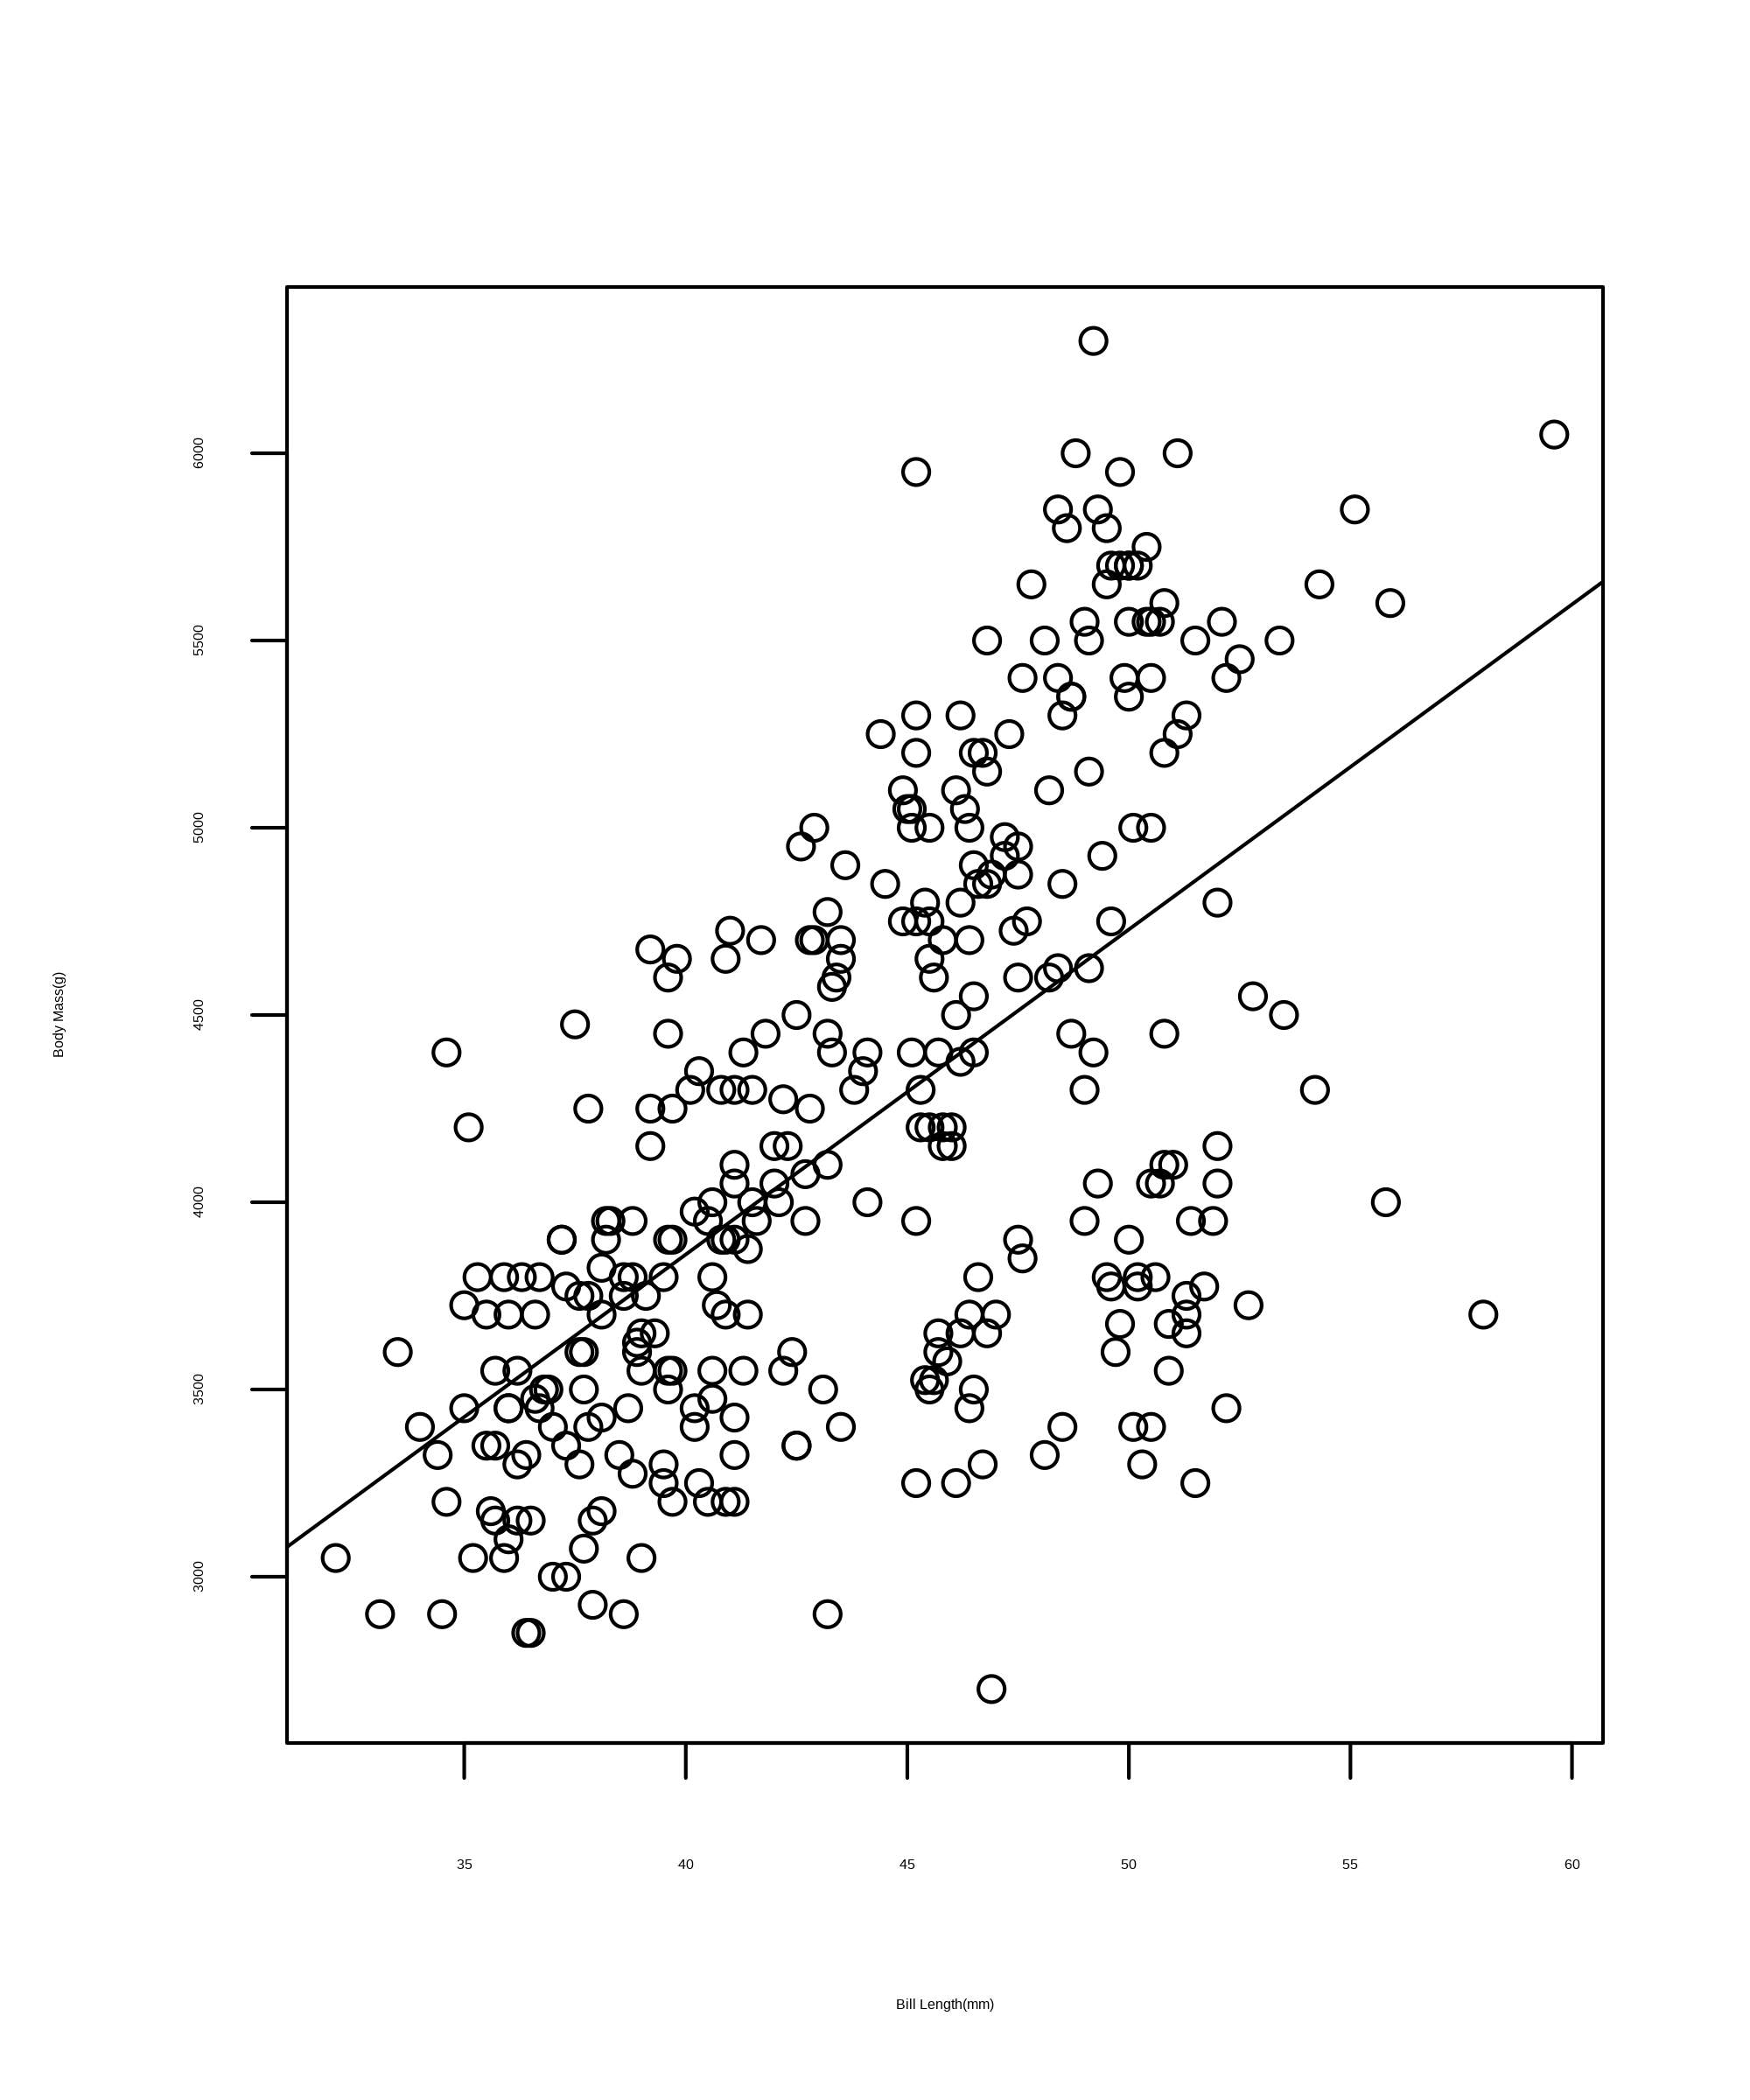
\includegraphics{visualizing-data-with-ggplot2_files/figure-pdf/unnamed-chunk-1-1.pdf}

}

\end{figure}

We get a blank plot. To add a layer you use \texttt{+}

\begin{Shaded}
\begin{Highlighting}[]
\FunctionTok{ggplot}\NormalTok{() }\SpecialCharTok{+}
  \FunctionTok{geom\_point}\NormalTok{(}\AttributeTok{data =}\NormalTok{ penguins,}
      \FunctionTok{aes}\NormalTok{(}\AttributeTok{x =}\NormalTok{ flipper\_length\_mm,}
          \AttributeTok{y =}\NormalTok{ body\_mass\_g))}
\end{Highlighting}
\end{Shaded}

\begin{figure}[H]

{\centering 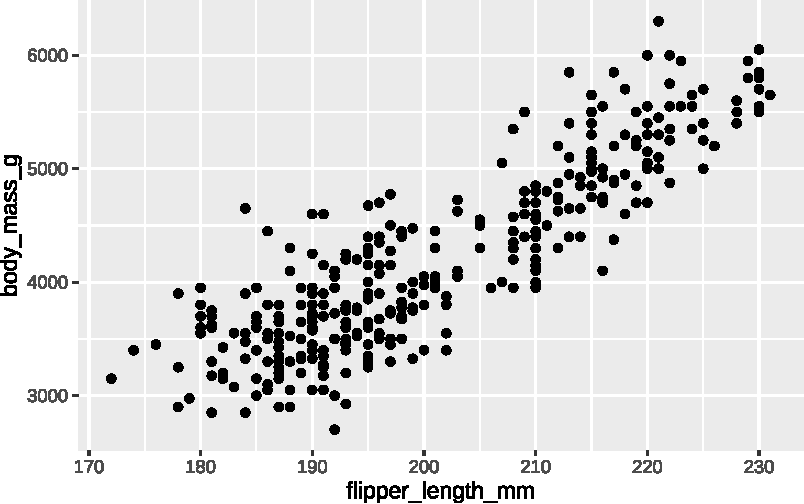
\includegraphics{visualizing-data-with-ggplot2_files/figure-pdf/scatter-basic-1.pdf}

}

\end{figure}

\marginnote{\begin{footnotesize}

To fit everything into the code blocks on the screen I have done.

\begin{Shaded}
\begin{Highlighting}[]
\FunctionTok{ggplot}\NormalTok{() }\SpecialCharTok{+}
  \FunctionTok{geom\_point}\NormalTok{(}\AttributeTok{data =}\NormalTok{ penguins,}
      \FunctionTok{aes}\NormalTok{(}\AttributeTok{x =}\NormalTok{ flipper\_length\_mm,}
          \AttributeTok{y =}\NormalTok{ body\_mass\_g))}
\end{Highlighting}
\end{Shaded}

You don't have to do this. Nothing terrible happens if you do, but I
want to save you some unnecessary keystrokes. Doing

\begin{Shaded}
\begin{Highlighting}[]
\FunctionTok{ggplot}\NormalTok{(penguings, }\FunctionTok{aes}\NormalTok{(}\AttributeTok{x =}\NormalTok{ body\_mass\_g, }\AttributeTok{y =}\NormalTok{ flipper\_length\_mm))}
\end{Highlighting}
\end{Shaded}

It is totally fine.

\end{footnotesize}}

If we want a histogram to show the distribution of bill length, we would
change the \texttt{geom} and the \texttt{aes}

\begin{Shaded}
\begin{Highlighting}[]
\FunctionTok{ggplot}\NormalTok{() }\SpecialCharTok{+}
\FunctionTok{geom\_histogram}\NormalTok{(}\AttributeTok{data =}\NormalTok{ penguins,}
             \FunctionTok{aes}\NormalTok{(}\AttributeTok{x =}\NormalTok{ bill\_length\_mm))}
\end{Highlighting}
\end{Shaded}

\begin{figure}[H]

{\centering \includegraphics{visualizing-data-with-ggplot2_files/figure-pdf/unnamed-chunk-4-1.pdf}

}

\end{figure}

If we want to add another kind of plot to our figure, we can add another
layer to our cake.

\begin{Shaded}
\begin{Highlighting}[]
\FunctionTok{ggplot}\NormalTok{() }\SpecialCharTok{+}
  \FunctionTok{geom\_point}\NormalTok{(}\AttributeTok{data =}\NormalTok{ penguins,}
      \FunctionTok{aes}\NormalTok{(}\AttributeTok{x =}\NormalTok{ flipper\_length\_mm,}
         \AttributeTok{y =}\NormalTok{ body\_mass\_g)) }\SpecialCharTok{+}
  \FunctionTok{geom\_smooth}\NormalTok{(}\AttributeTok{data =}\NormalTok{ penguins,}
     \FunctionTok{aes}\NormalTok{(}\AttributeTok{x =}\NormalTok{ flipper\_length\_mm,}
         \AttributeTok{y =}\NormalTok{ body\_mass\_g)) }\CommentTok{\# adds a best fit line}
\end{Highlighting}
\end{Shaded}

\begin{figure}[H]

{\centering \includegraphics{visualizing-data-with-ggplot2_files/figure-pdf/unnamed-chunk-5-1.pdf}

}

\end{figure}

We want to give our audience a better understanding of what the
variables are, so we should add more informative labels.

\begin{Shaded}
\begin{Highlighting}[]
\FunctionTok{ggplot}\NormalTok{() }\SpecialCharTok{+}
  \FunctionTok{geom\_point}\NormalTok{( }\AttributeTok{data =}\NormalTok{ penguins,}
            \FunctionTok{aes}\NormalTok{(}\AttributeTok{x =}\NormalTok{ flipper\_length\_mm, }\AttributeTok{y =}\NormalTok{ body\_mass\_g)) }\SpecialCharTok{+}
  \FunctionTok{geom\_smooth}\NormalTok{(}\AttributeTok{data =}\NormalTok{ penguins,}
           \FunctionTok{aes}\NormalTok{(}\AttributeTok{x =}\NormalTok{ flipper\_length\_mm, }\AttributeTok{y =}\NormalTok{ body\_mass\_g)) }\SpecialCharTok{+}
  \FunctionTok{labs}\NormalTok{(}\AttributeTok{x =} \StringTok{"Flipper Length(mm)"}\NormalTok{, }\AttributeTok{y =} \StringTok{"Body Mass(g)"}\NormalTok{)}
\end{Highlighting}
\end{Shaded}

\begin{figure}[H]

{\centering 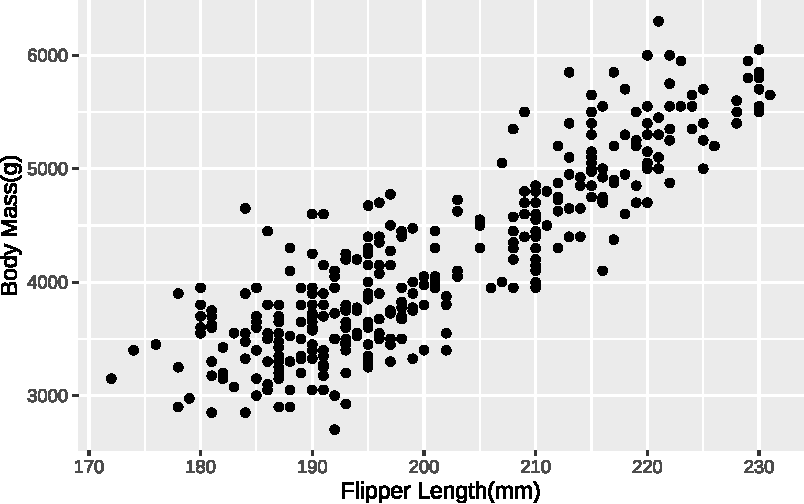
\includegraphics{visualizing-data-with-ggplot2_files/figure-pdf/scatter-plot-labs-1.pdf}

}

\end{figure}

So far, we have only done stuff working within \texttt{aes}. Here is one
of the most common mistakes when working in \texttt{ggplot}.

\begin{Shaded}
\begin{Highlighting}[]
\FunctionTok{ggplot}\NormalTok{() }\SpecialCharTok{+}
  \FunctionTok{geom\_point}\NormalTok{(}\AttributeTok{data =}\NormalTok{ penguins,}
              \FunctionTok{aes}\NormalTok{(}\AttributeTok{x =}\NormalTok{ flipper\_length\_mm,}
                  \AttributeTok{y =}\NormalTok{ body\_mass\_g,}
                  \AttributeTok{color =} \StringTok{"blue"}\NormalTok{)) }\SpecialCharTok{+}
  \FunctionTok{labs}\NormalTok{(}\AttributeTok{x =} \StringTok{"Flipper Length(mm)"}\NormalTok{, }\AttributeTok{y =} \StringTok{"Body Mass(g)"}\NormalTok{)}
\end{Highlighting}
\end{Shaded}

\begin{figure}[H]

{\centering 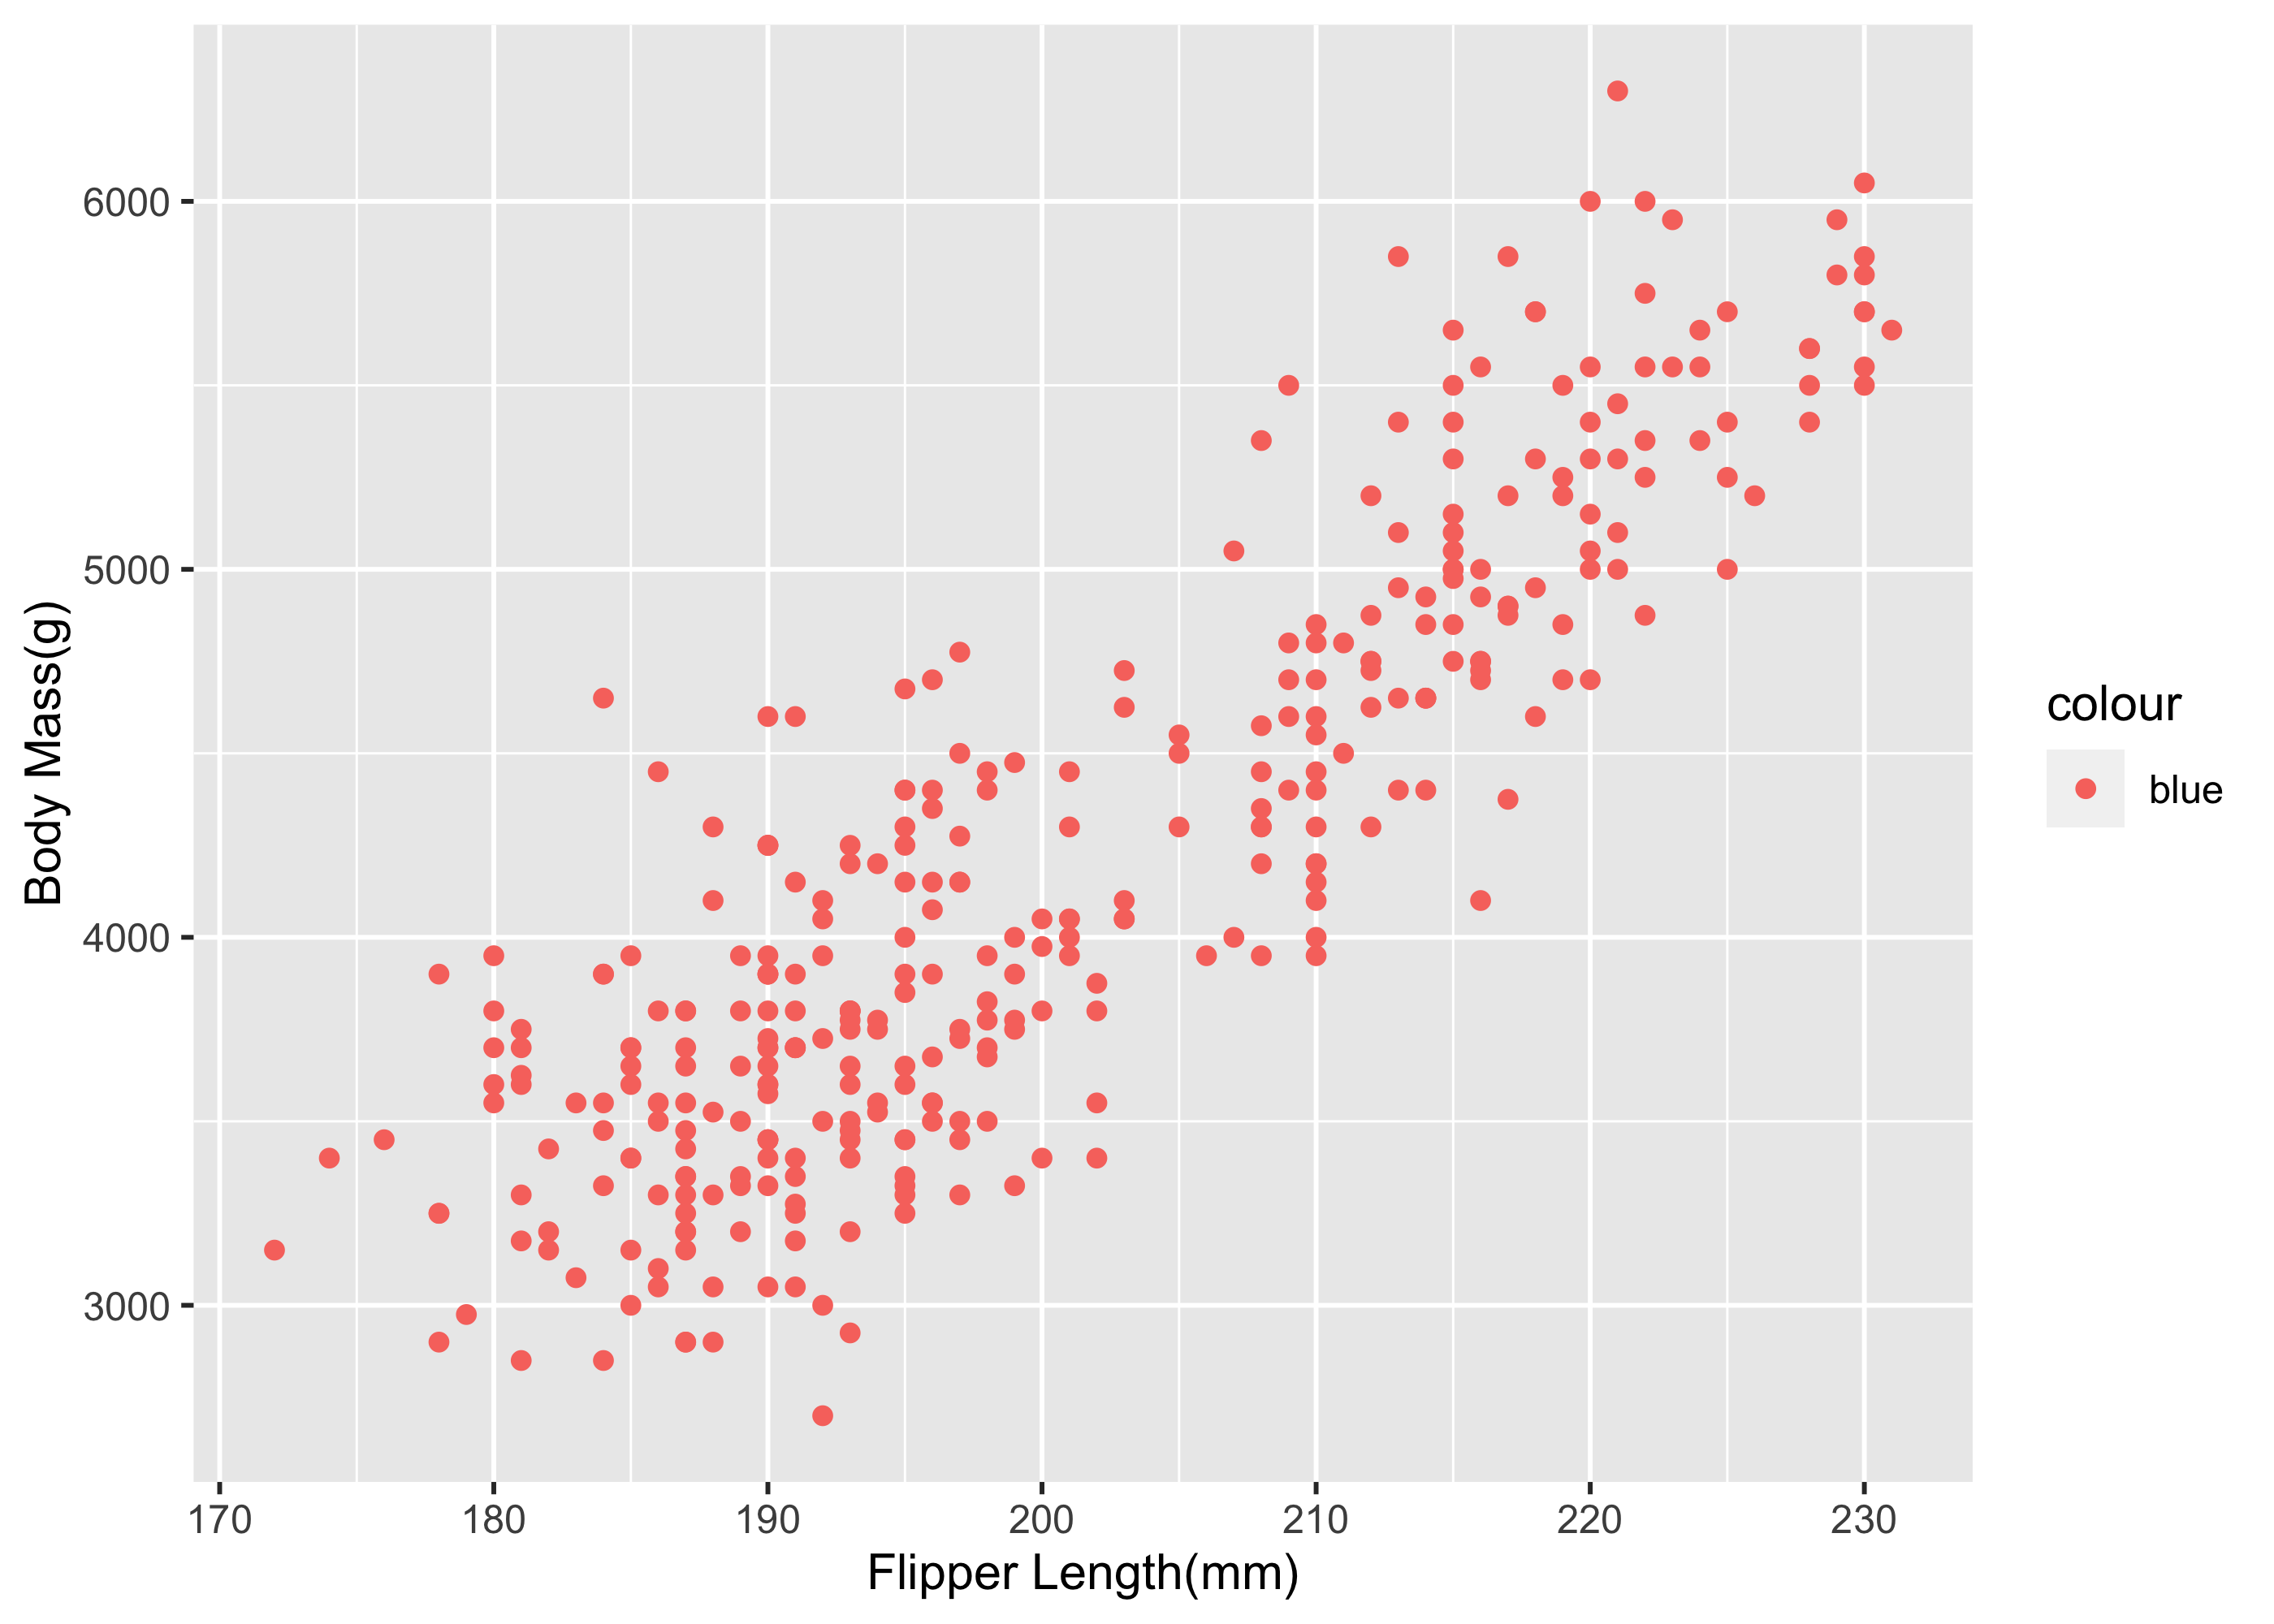
\includegraphics{visualizing-data-with-ggplot2_files/figure-pdf/mistake-easy-1.pdf}

}

\end{figure}

I wanted to change the color of the dots. However, I did this in the
\texttt{aes()}. If you look back, you will remember that \texttt{aes}
will look to put stuff in your plots based on \textbf{columns} in your
dataset. So to change the look of your plot, you need to do it
\textbf{outside} of \texttt{aes()}.

\begin{Shaded}
\begin{Highlighting}[]
\FunctionTok{ggplot}\NormalTok{() }\SpecialCharTok{+}
  \FunctionTok{geom\_point}\NormalTok{(}\AttributeTok{data =}\NormalTok{ penguins,}
            \FunctionTok{aes}\NormalTok{(}\AttributeTok{x =}\NormalTok{ flipper\_length\_mm,}
           \AttributeTok{y =}\NormalTok{ body\_mass\_g), }\AttributeTok{color =} \StringTok{"blue"}\NormalTok{) }\SpecialCharTok{+}
  \FunctionTok{labs}\NormalTok{(}\AttributeTok{x =} \StringTok{"Flipper Length(mm)"}\NormalTok{, }\AttributeTok{y =} \StringTok{"Body Mass(g)"}\NormalTok{)}
\end{Highlighting}
\end{Shaded}

\begin{figure}[H]

{\centering 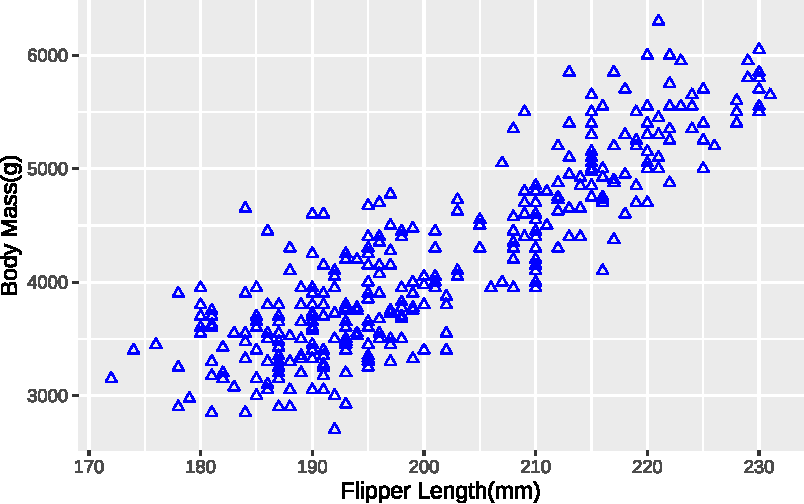
\includegraphics{visualizing-data-with-ggplot2_files/figure-pdf/real-changes-1.pdf}

}

\end{figure}

Notice that we have been working within the various \texttt{geoms}. This
gets tedious very quickly when we have more than one \texttt{geom}. When
you work inside the individual \texttt{geoms} this is called working
locally, meaning the other \texttt{geoms} do not inherit any of the
stuff in the other. The good news is that there is a global option where
each \texttt{geom} inherits the data and aesthetics from the global
options, and you do not need to specify them.

\begin{Shaded}
\begin{Highlighting}[]
\FunctionTok{ggplot}\NormalTok{(penguins,}
       \FunctionTok{aes}\NormalTok{(}\AttributeTok{x =}\NormalTok{ flipper\_length\_mm,}
           \AttributeTok{y =}\NormalTok{ body\_mass\_g)) }\SpecialCharTok{+}
\FunctionTok{geom\_point}\NormalTok{() }\SpecialCharTok{+}
\FunctionTok{geom\_smooth}\NormalTok{() }\SpecialCharTok{+} 
\FunctionTok{labs}\NormalTok{(}\AttributeTok{x =} \StringTok{"Flipper Length(mm)"}\NormalTok{, }\AttributeTok{y =} \StringTok{"Body Mass(g)"}\NormalTok{)}
\end{Highlighting}
\end{Shaded}

\begin{figure}[H]

{\centering 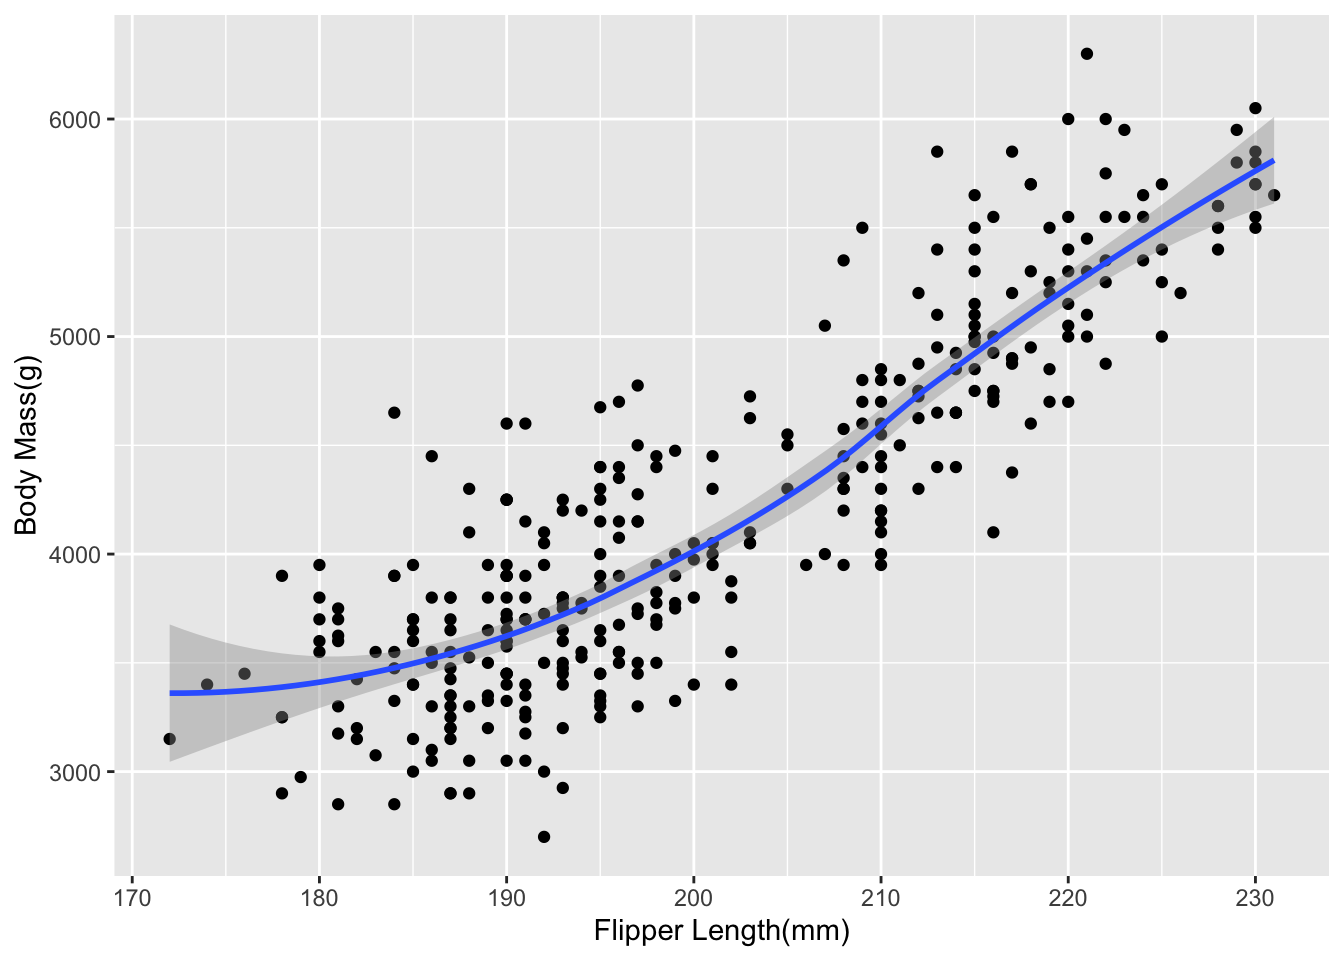
\includegraphics{visualizing-data-with-ggplot2_files/figure-pdf/unnamed-chunk-6-1.pdf}

}

\end{figure}

Notice that we did not have to tell the geoms anything. If we wanted to
specify more specific options for each geom, we can.

In the case of the penguins dataset, there are subgroups that tell an
important story about the relationship between flipper length and body
mass. We can visualize those easily.

\begin{Shaded}
\begin{Highlighting}[]
\FunctionTok{ggplot}\NormalTok{(penguins,}
       \FunctionTok{aes}\NormalTok{(}\AttributeTok{x =}\NormalTok{ flipper\_length\_mm,}
           \AttributeTok{y =}\NormalTok{ body\_mass\_g,}
          \AttributeTok{color =}\NormalTok{ species,}
          \AttributeTok{shape =}\NormalTok{ species)) }\SpecialCharTok{+}
\FunctionTok{geom\_point}\NormalTok{() }\SpecialCharTok{+}
\FunctionTok{labs}\NormalTok{(}\AttributeTok{x =} \StringTok{"Flipper Length(mm)"}\NormalTok{, }\AttributeTok{y =} \StringTok{"Body Mass(g)"}\NormalTok{)}
\end{Highlighting}
\end{Shaded}

\begin{figure}[H]

{\centering 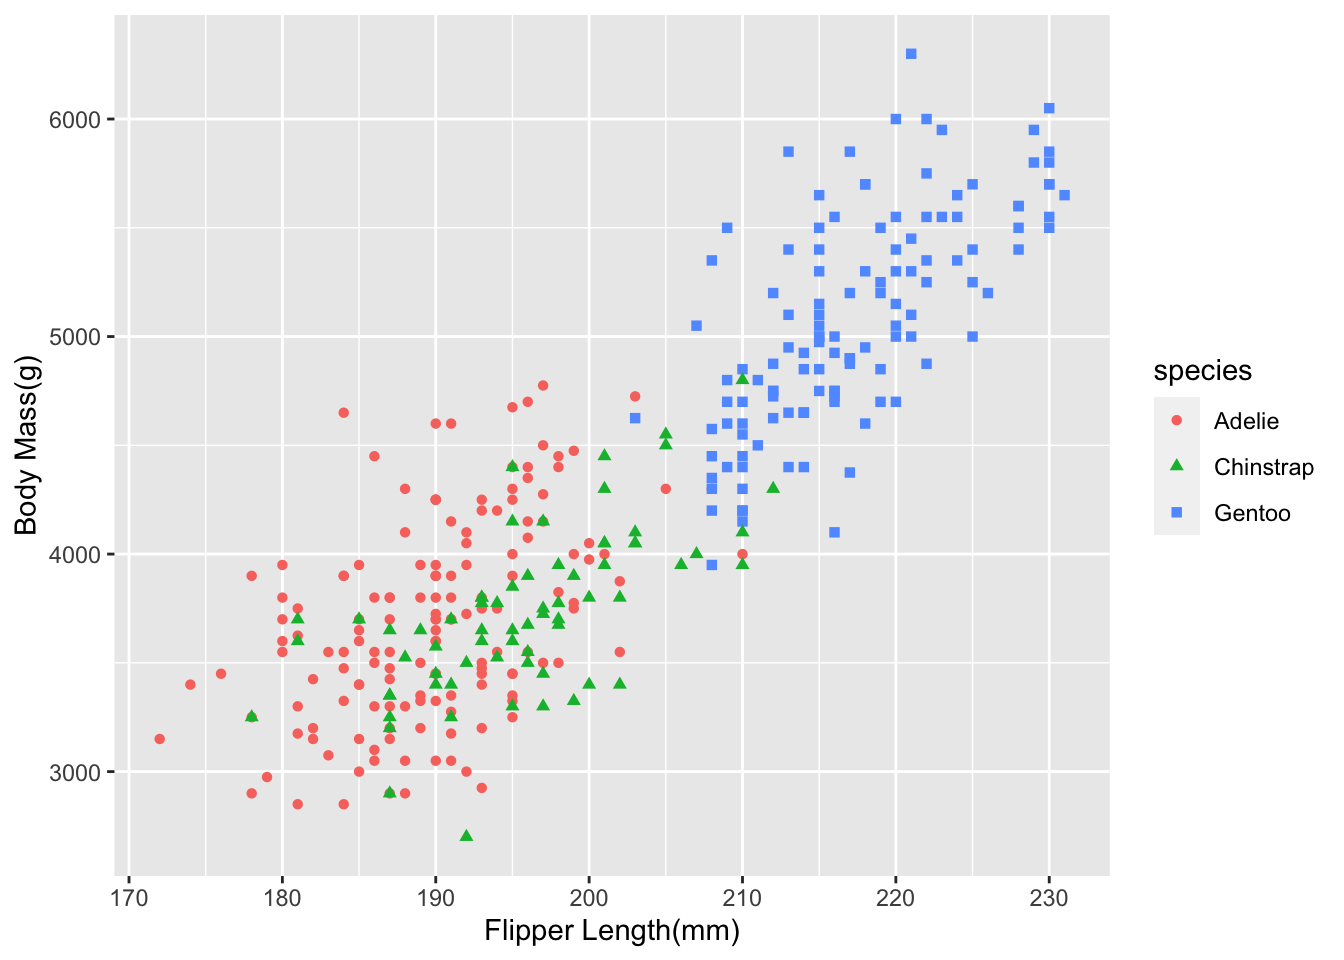
\includegraphics{visualizing-data-with-ggplot2_files/figure-pdf/unnamed-chunk-7-1.pdf}

}

\end{figure}

Here we are using two of the other options for \texttt{ggplot}
\texttt{shape} and \texttt{color}

This works slightly differently for things like histograms or density
plots instead of \texttt{color} we use \texttt{fill}

\begin{Shaded}
\begin{Highlighting}[]
\FunctionTok{ggplot}\NormalTok{(}\AttributeTok{data =}\NormalTok{ penguins, }\FunctionTok{aes}\NormalTok{(}\AttributeTok{x =}\NormalTok{ bill\_length\_mm, }\AttributeTok{fill =}\NormalTok{ species)) }\SpecialCharTok{+}
\FunctionTok{geom\_density}\NormalTok{() }\SpecialCharTok{+}
\FunctionTok{labs}\NormalTok{(}\AttributeTok{x =} \StringTok{"Bill Length(mm)"}\NormalTok{)}
\end{Highlighting}
\end{Shaded}

\begin{figure}[H]

{\centering 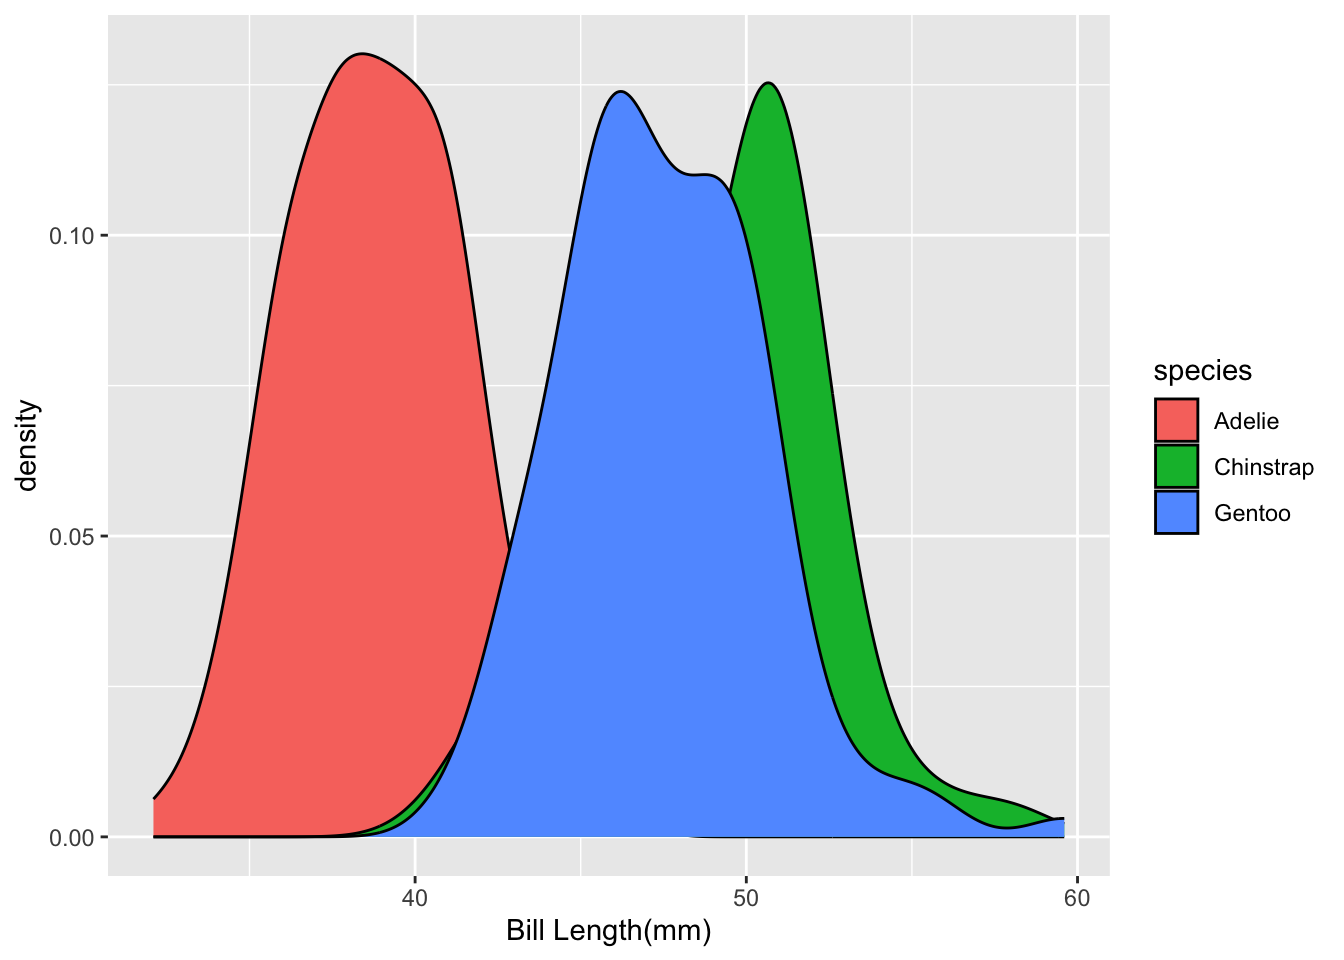
\includegraphics{visualizing-data-with-ggplot2_files/figure-pdf/unnamed-chunk-8-1.pdf}

}

\end{figure}

Notice that it can be hard to see the parts of the distribution in the
middle. We can fix that by changing the transparency in the geom

\begin{Shaded}
\begin{Highlighting}[]
\FunctionTok{ggplot}\NormalTok{(}\AttributeTok{data =}\NormalTok{ penguins, }\FunctionTok{aes}\NormalTok{(}\AttributeTok{x =}\NormalTok{ bill\_length\_mm, }\AttributeTok{fill =}\NormalTok{ species)) }\SpecialCharTok{+}
\FunctionTok{geom\_density}\NormalTok{(}\AttributeTok{alpha =} \FloatTok{0.4}\NormalTok{) }\SpecialCharTok{+}
\FunctionTok{labs}\NormalTok{(}\AttributeTok{x =} \StringTok{"Bill Length(mm)"}\NormalTok{)}
\end{Highlighting}
\end{Shaded}

\begin{figure}[H]

{\centering 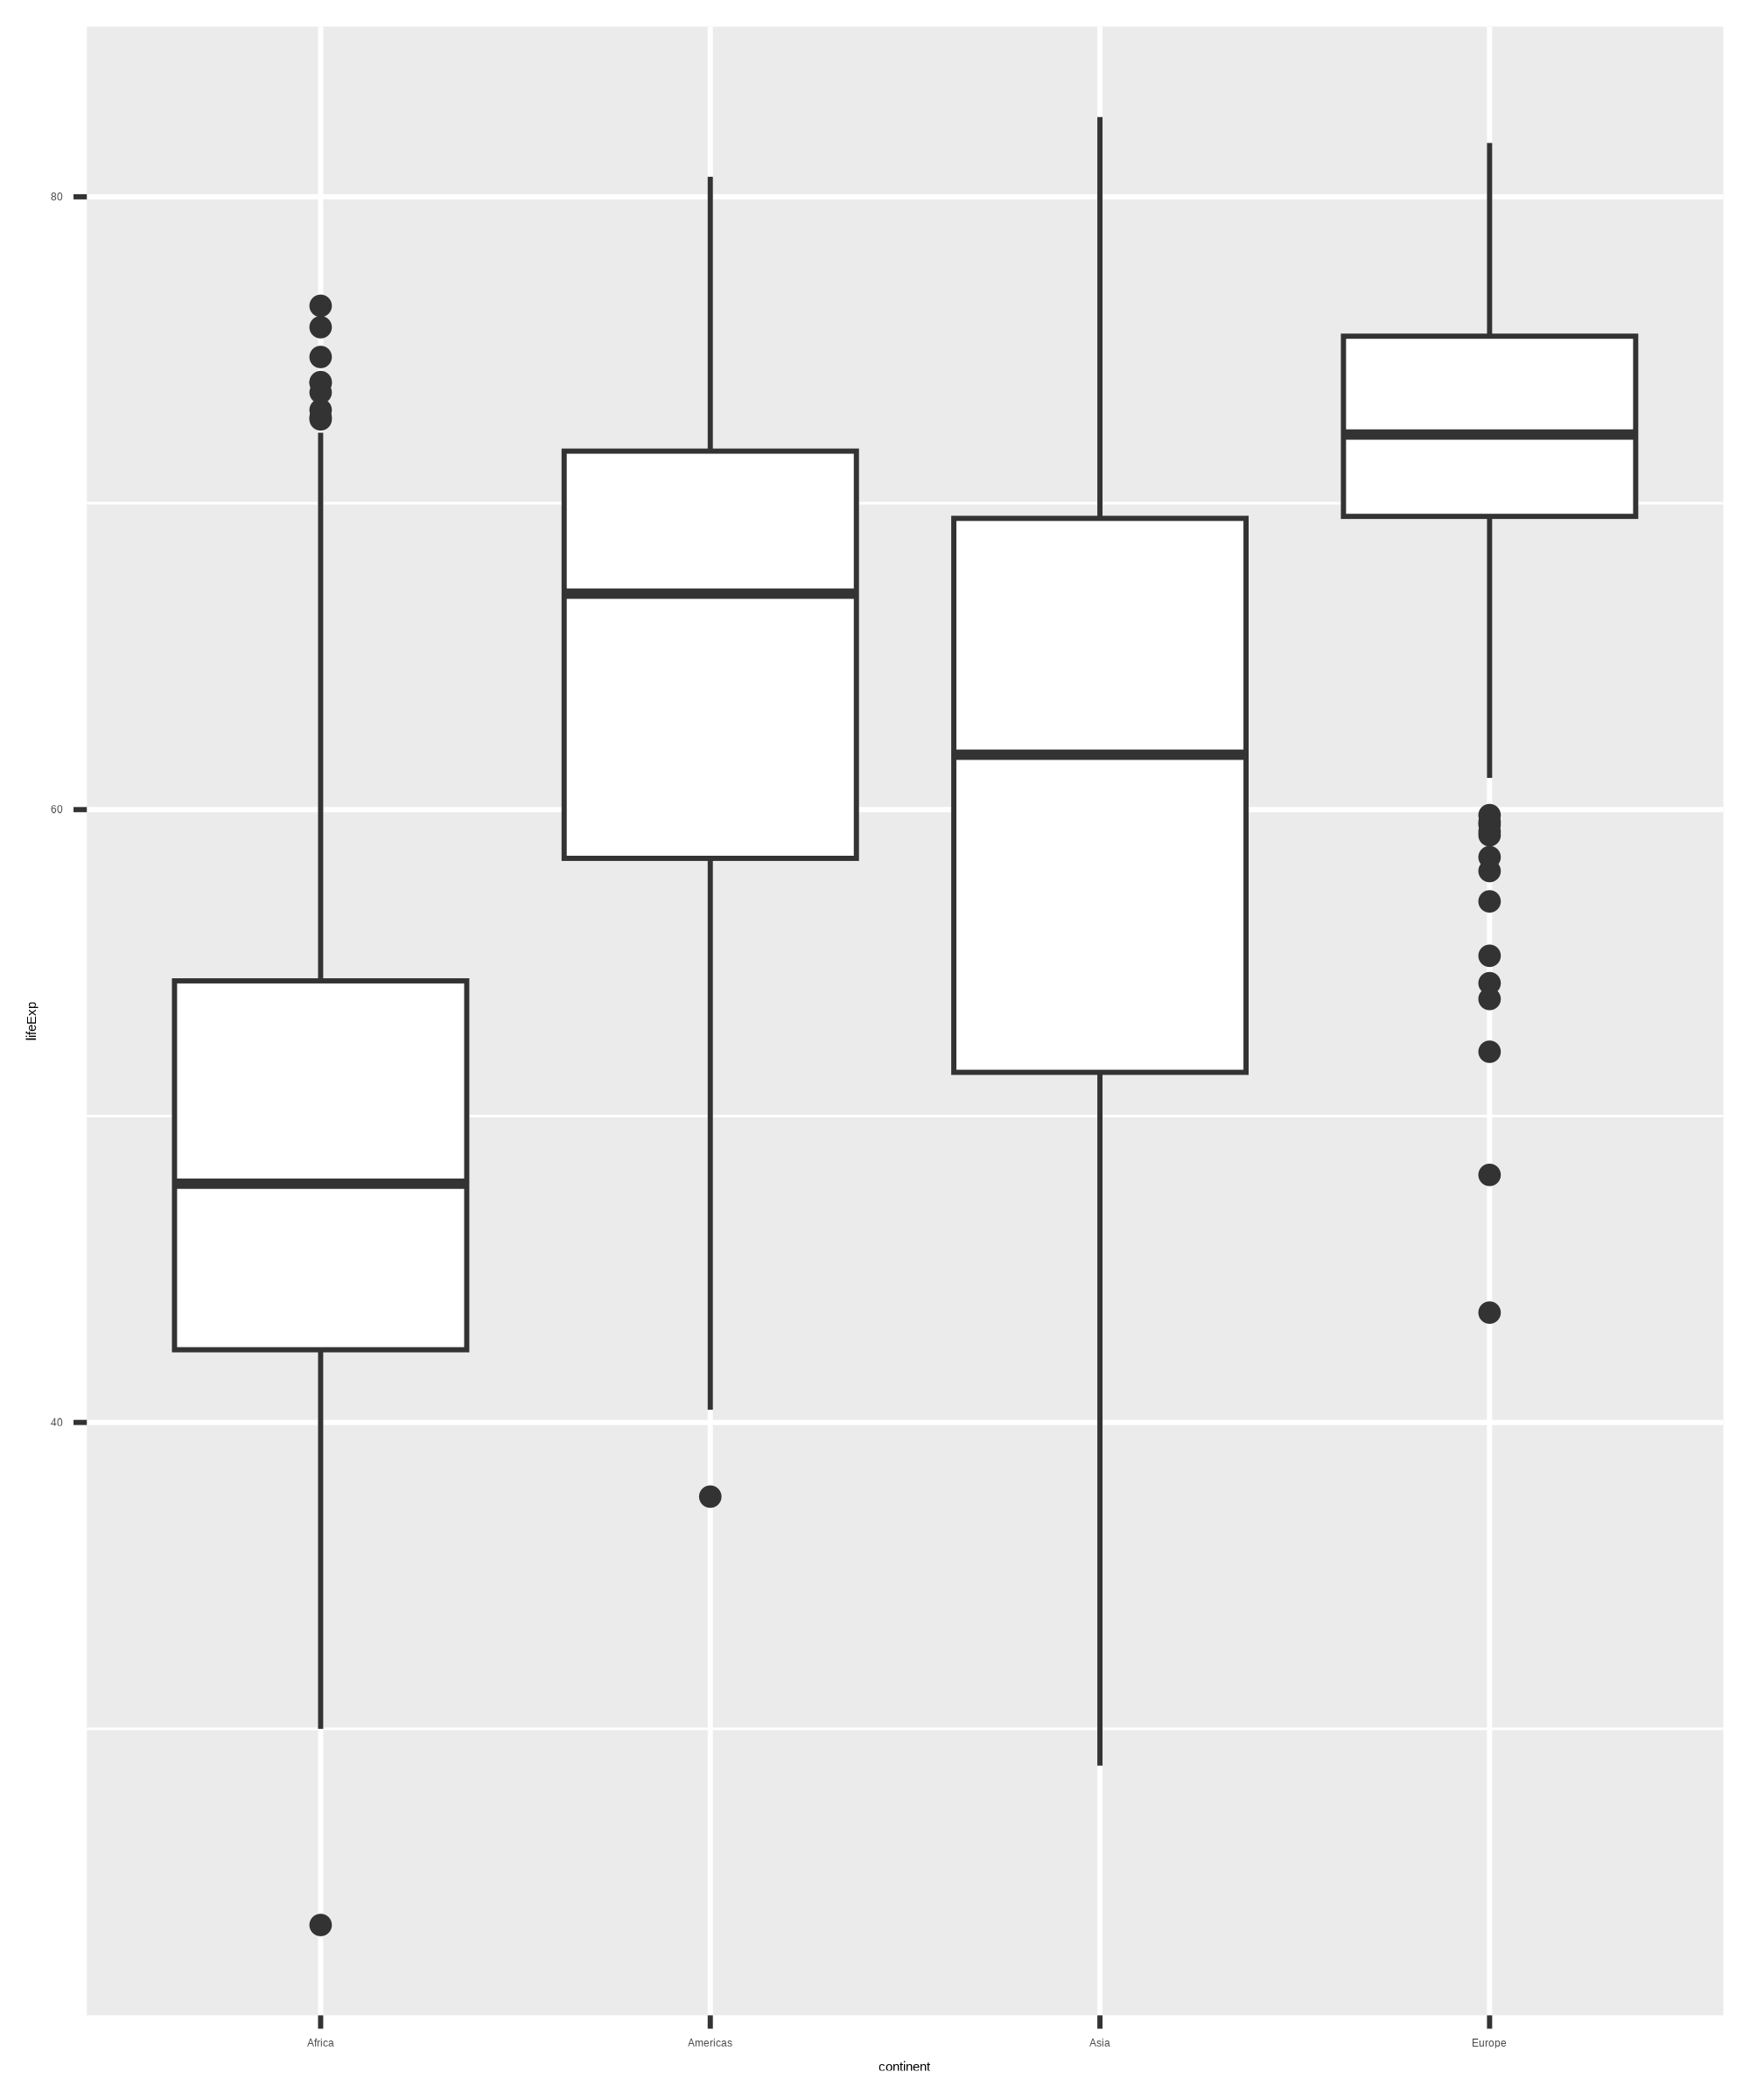
\includegraphics{visualizing-data-with-ggplot2_files/figure-pdf/unnamed-chunk-9-1.pdf}

}

\end{figure}

Density plots are just another way of visualizing distributions. They
use math to plot the distribution, whereas histograms group numbers into
equal-sized bins.

\hypertarget{scales}{%
\subsection{Scales}\label{scales}}

The \texttt{scale\_*()} components control the properties of all
theaesthetic dimensions mapped to the data. It means that it controls
where things go in the plot and what they look like.

The extensions (\texttt{*}) can be filled by e.g.:

\begin{itemize}
\item
  \texttt{continuous()}, \texttt{discrete()}, \texttt{reverse()},
  \texttt{log10()}, \texttt{sqrt()}, \texttt{date()} for positions
\item
  \texttt{continuous()}, \texttt{discrete()}, \texttt{manual()},
  \texttt{gradient()}, \texttt{gradient2()}, \texttt{brewer()} for
  colors
\item
  \texttt{continuous()}, \texttt{discrete()}, \texttt{manual()},
  \texttt{ordinal()}, \texttt{area()}, \texttt{date()} for sizes
\item
  \texttt{continuous()}, \texttt{discrete()}, \texttt{manual()},
  \texttt{ordinal()} for shapes
\item
  \texttt{continuous()}, \texttt{discrete()}, \texttt{manual()},
  \texttt{ordinal()}, \texttt{date()} for transparency
\end{itemize}

\begin{center}\rule{0.5\linewidth}{0.5pt}\end{center}

\begin{figure}

{\centering \includegraphics{pics/continuous_discrete.png}

}

\caption{Illustration by
\href{https://github.com/allisonhorst/stats-illustrations}{Allison
Horst}}

\end{figure}

\hypertarget{continuous-vs.-discrete-in-ggplot2}{%
\section{\texorpdfstring{Continuous vs.~Discrete in
\texttt{ggplot2}}{Continuous vs.~Discrete in ggplot2}}\label{continuous-vs.-discrete-in-ggplot2}}

\begin{figure}

\begin{minipage}[t]{0.50\linewidth}

{\centering 

\hypertarget{continuous-quantitative-or-numerical-data}{%
\section{\texorpdfstring{Continuous:quantitative or numerical
data}{Continuous: quantitative or numerical data}}\label{continuous-quantitative-or-numerical-data}}

\begin{itemize}
\tightlist
\item
  height
\item
  weight
\item
  age
\item
  counts
\end{itemize}

}

\end{minipage}%
%
\begin{minipage}[t]{0.50\linewidth}

{\centering 

\hypertarget{discrete-qualitative-or-categorical-data}{%
\section{\texorpdfstring{Discrete:qualitative or categorical
data}{Discrete: qualitative or categorical data}}\label{discrete-qualitative-or-categorical-data}}

\begin{itemize}
\tightlist
\item
  species
\item
  sex
\item
  study sites
\item
  age group
\end{itemize}

}

\end{minipage}%

\end{figure}

\hypertarget{continuous-vs.-discrete-in-ggplot2-1}{%
\section{Continuous vs.~Discrete in
\{ggplot2\}}\label{continuous-vs.-discrete-in-ggplot2-1}}

\begin{figure}

\begin{minipage}[t]{0.50\linewidth}

{\centering 

\hypertarget{continuous-quantitative-or-numerical-data-1}{%
\section{\texorpdfstring{Continuous:quantitative or numerical
data}{Continuous: quantitative or numerical data}}\label{continuous-quantitative-or-numerical-data-1}}

\begin{itemize}
\tightlist
\item
  height (continuous)
\item
  weight (continuous)
\item
  age (continuous or discrete)
\item
  counts (discrete)
\end{itemize}

}

\end{minipage}%
%
\begin{minipage}[t]{0.50\linewidth}

{\centering 

\hypertarget{discrete-qualitative-or-categorical-data-1}{%
\section{\texorpdfstring{Discrete:qualitative or categorical
data}{Discrete: qualitative or categorical data}}\label{discrete-qualitative-or-categorical-data-1}}

\begin{itemize}
\tightlist
\item
  species (nominal)
\item
  sex (nominal)
\item
  study site (nominal or ordinal)
\item
  age group (ordinal)
\end{itemize}

}

\end{minipage}%

\end{figure}

\begin{Shaded}
\begin{Highlighting}[]
\FunctionTok{ggplot}\NormalTok{(penguins,}
      \FunctionTok{aes}\NormalTok{(}\AttributeTok{x =}\NormalTok{ flipper\_length\_mm,}
          \AttributeTok{y =}\NormalTok{ body\_mass\_g,}
          \AttributeTok{color =}\NormalTok{ species,}
          \AttributeTok{shape =}\NormalTok{ species)) }\SpecialCharTok{+}
\FunctionTok{geom\_point}\NormalTok{() }\SpecialCharTok{+}
\FunctionTok{labs}\NormalTok{(}\AttributeTok{x =} \StringTok{"Flipper Length(mm)"}\NormalTok{, }\AttributeTok{y =} \StringTok{"Body Mass(g)"}\NormalTok{) }\SpecialCharTok{+}
\FunctionTok{scale\_x\_continuous}\NormalTok{(}\AttributeTok{limits =} \FunctionTok{c}\NormalTok{(}\DecValTok{170}\NormalTok{, }\DecValTok{240}\NormalTok{))}
\end{Highlighting}
\end{Shaded}

\begin{figure}[H]

{\centering 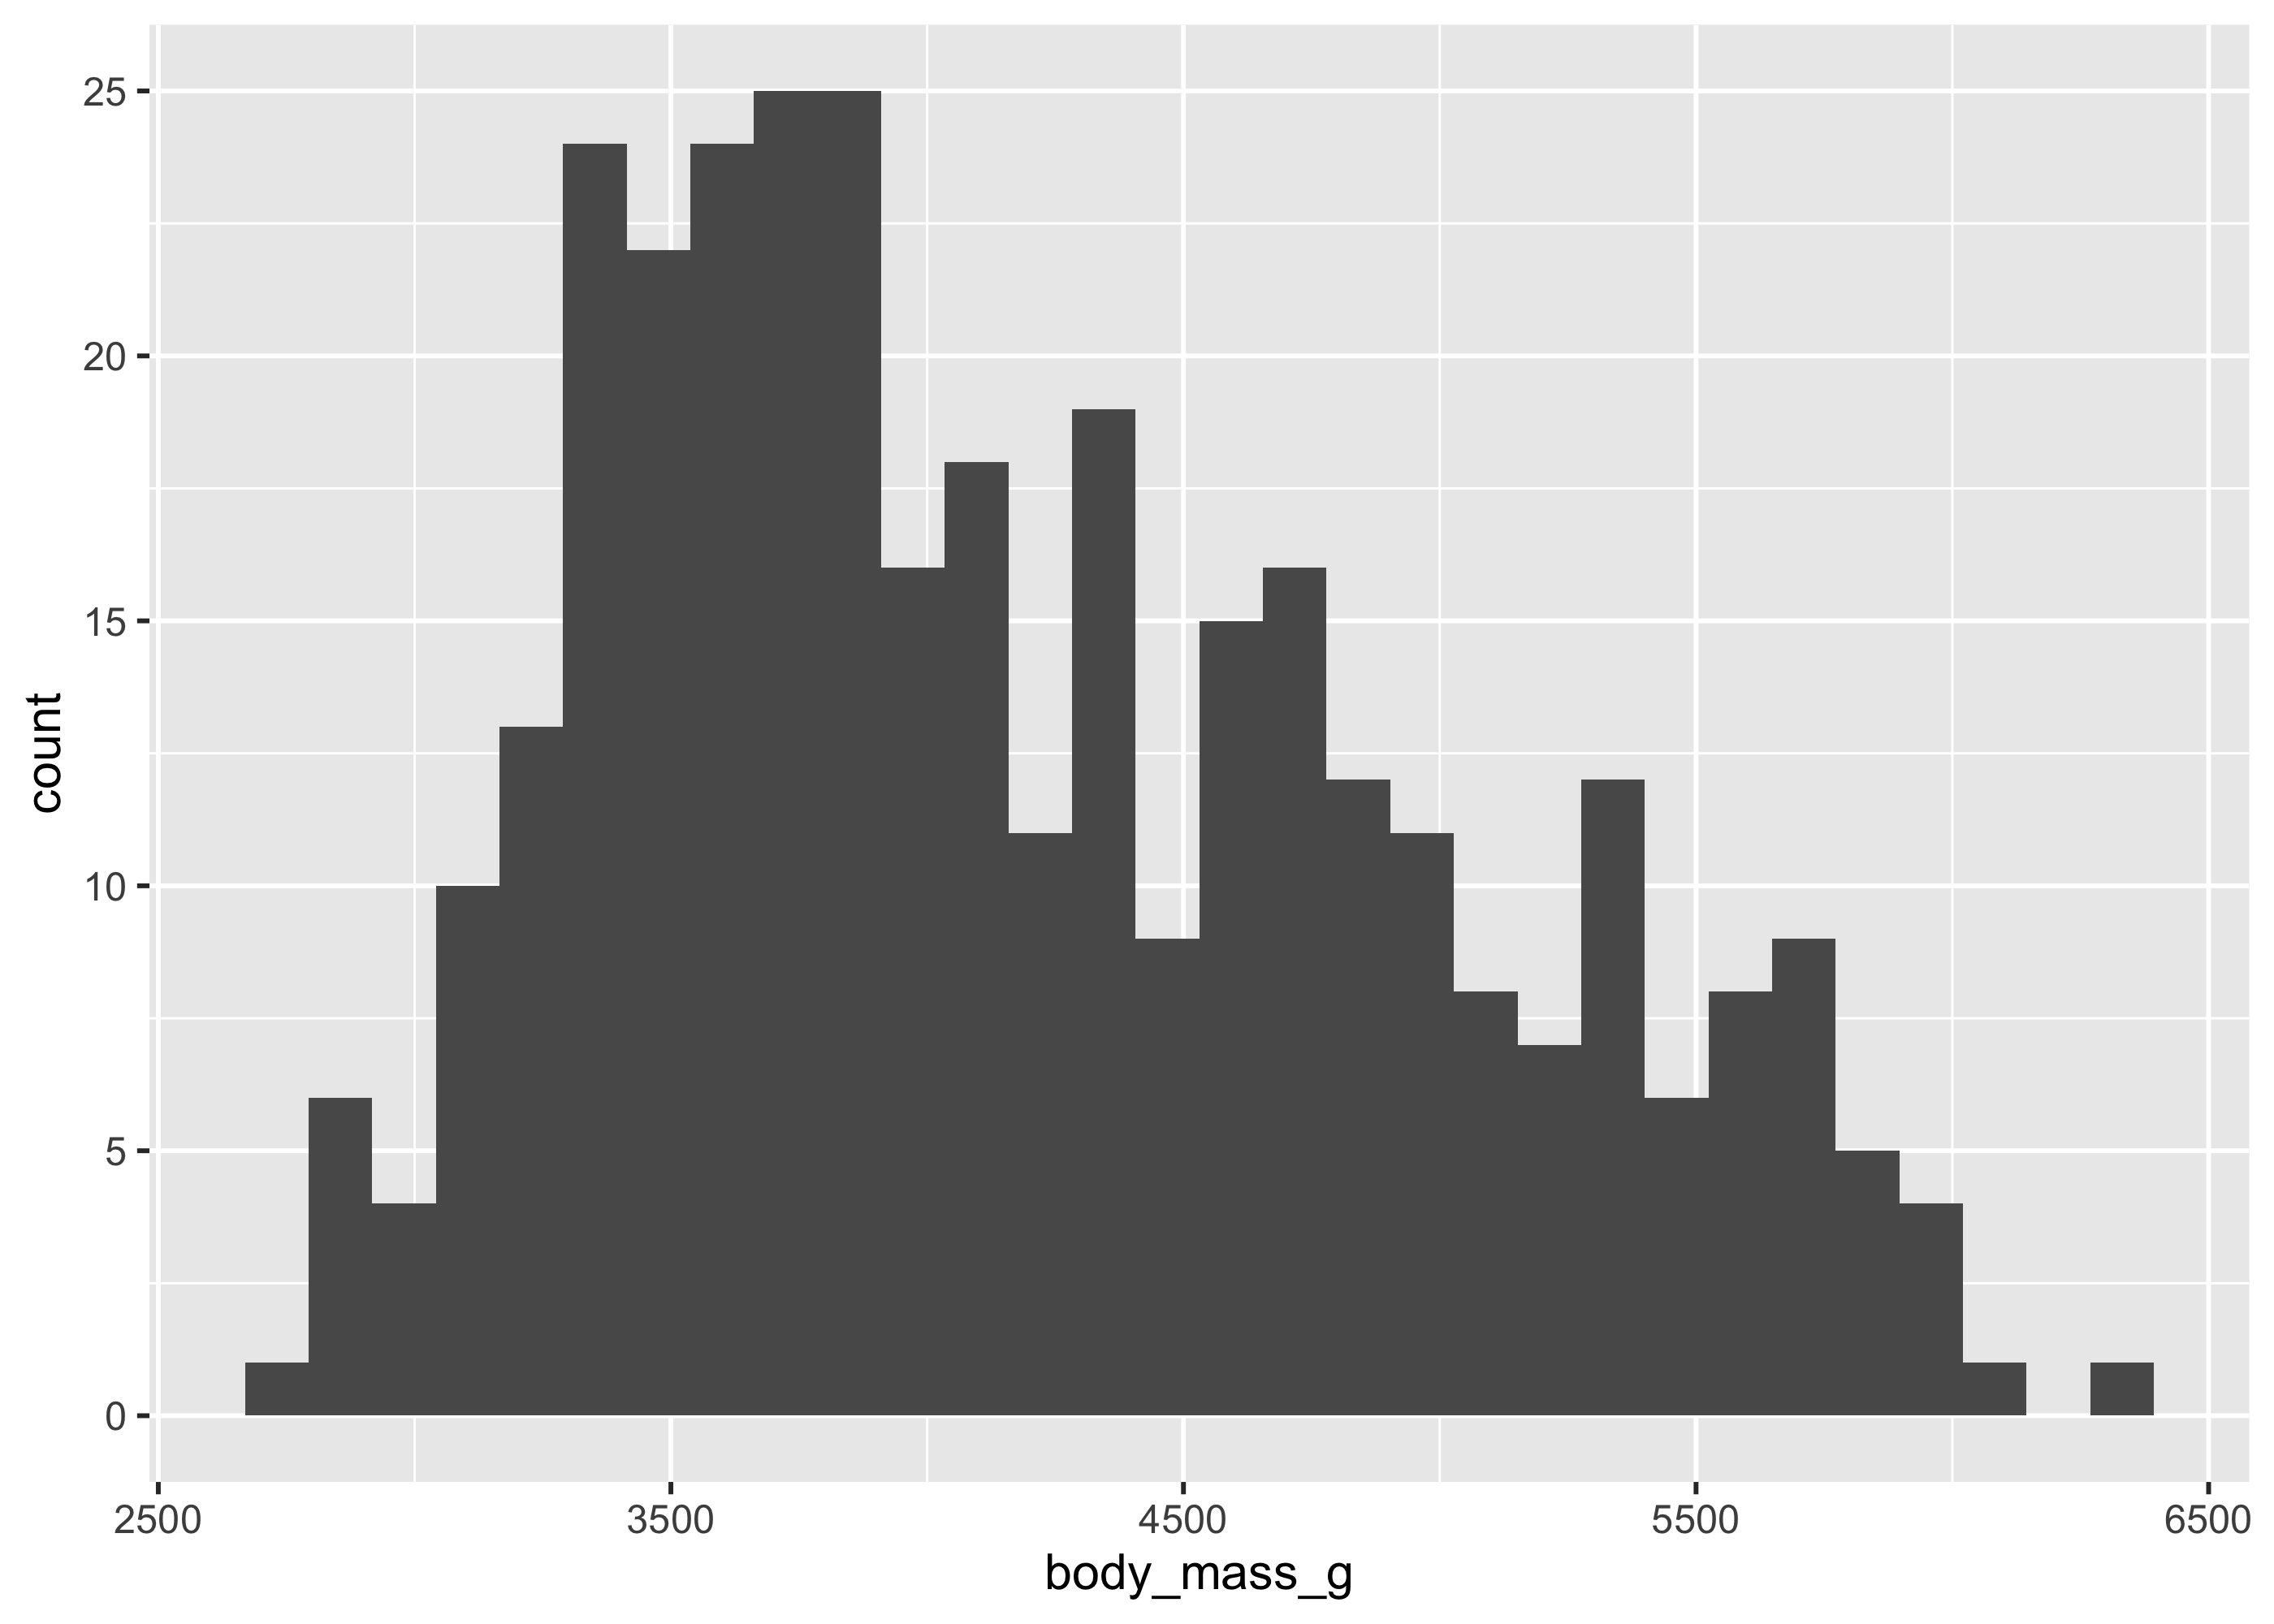
\includegraphics{visualizing-data-with-ggplot2_files/figure-pdf/unnamed-chunk-10-1.pdf}

}

\end{figure}

Scales also apply to color scales. The default colors in \texttt{R} out
of the box are not always the prettiest, and when you present figures to
a professional audience, you generally want to customize them. There are
also accessibility issues. The default colors may not be
colorblind-friendly. One popular colorblind-friendly palette is the
viridis color palette. I like the MetBrewer package and use it all the
time in my work.

\begin{Shaded}
\begin{Highlighting}[]
\FunctionTok{ggplot}\NormalTok{(penguins,}
      \FunctionTok{aes}\NormalTok{(}\AttributeTok{x =}\NormalTok{ flipper\_length\_mm,}
          \AttributeTok{y =}\NormalTok{ body\_mass\_g,}
          \AttributeTok{color =}\NormalTok{ species,}
          \AttributeTok{shape =}\NormalTok{ species)) }\SpecialCharTok{+}
\FunctionTok{geom\_point}\NormalTok{() }\SpecialCharTok{+}
\FunctionTok{labs}\NormalTok{(}\AttributeTok{x =} \StringTok{"Flipper Length(mm)"}\NormalTok{, }\AttributeTok{y =} \StringTok{"Body Mass(g)"}\NormalTok{) }\SpecialCharTok{+}
\FunctionTok{scale\_color\_met\_d}\NormalTok{(}\AttributeTok{name =} \StringTok{"Demuth"}\NormalTok{) }\CommentTok{\# if this color scheme looks familiar, this is what my slides use}
\end{Highlighting}
\end{Shaded}

\begin{figure}[H]

{\centering 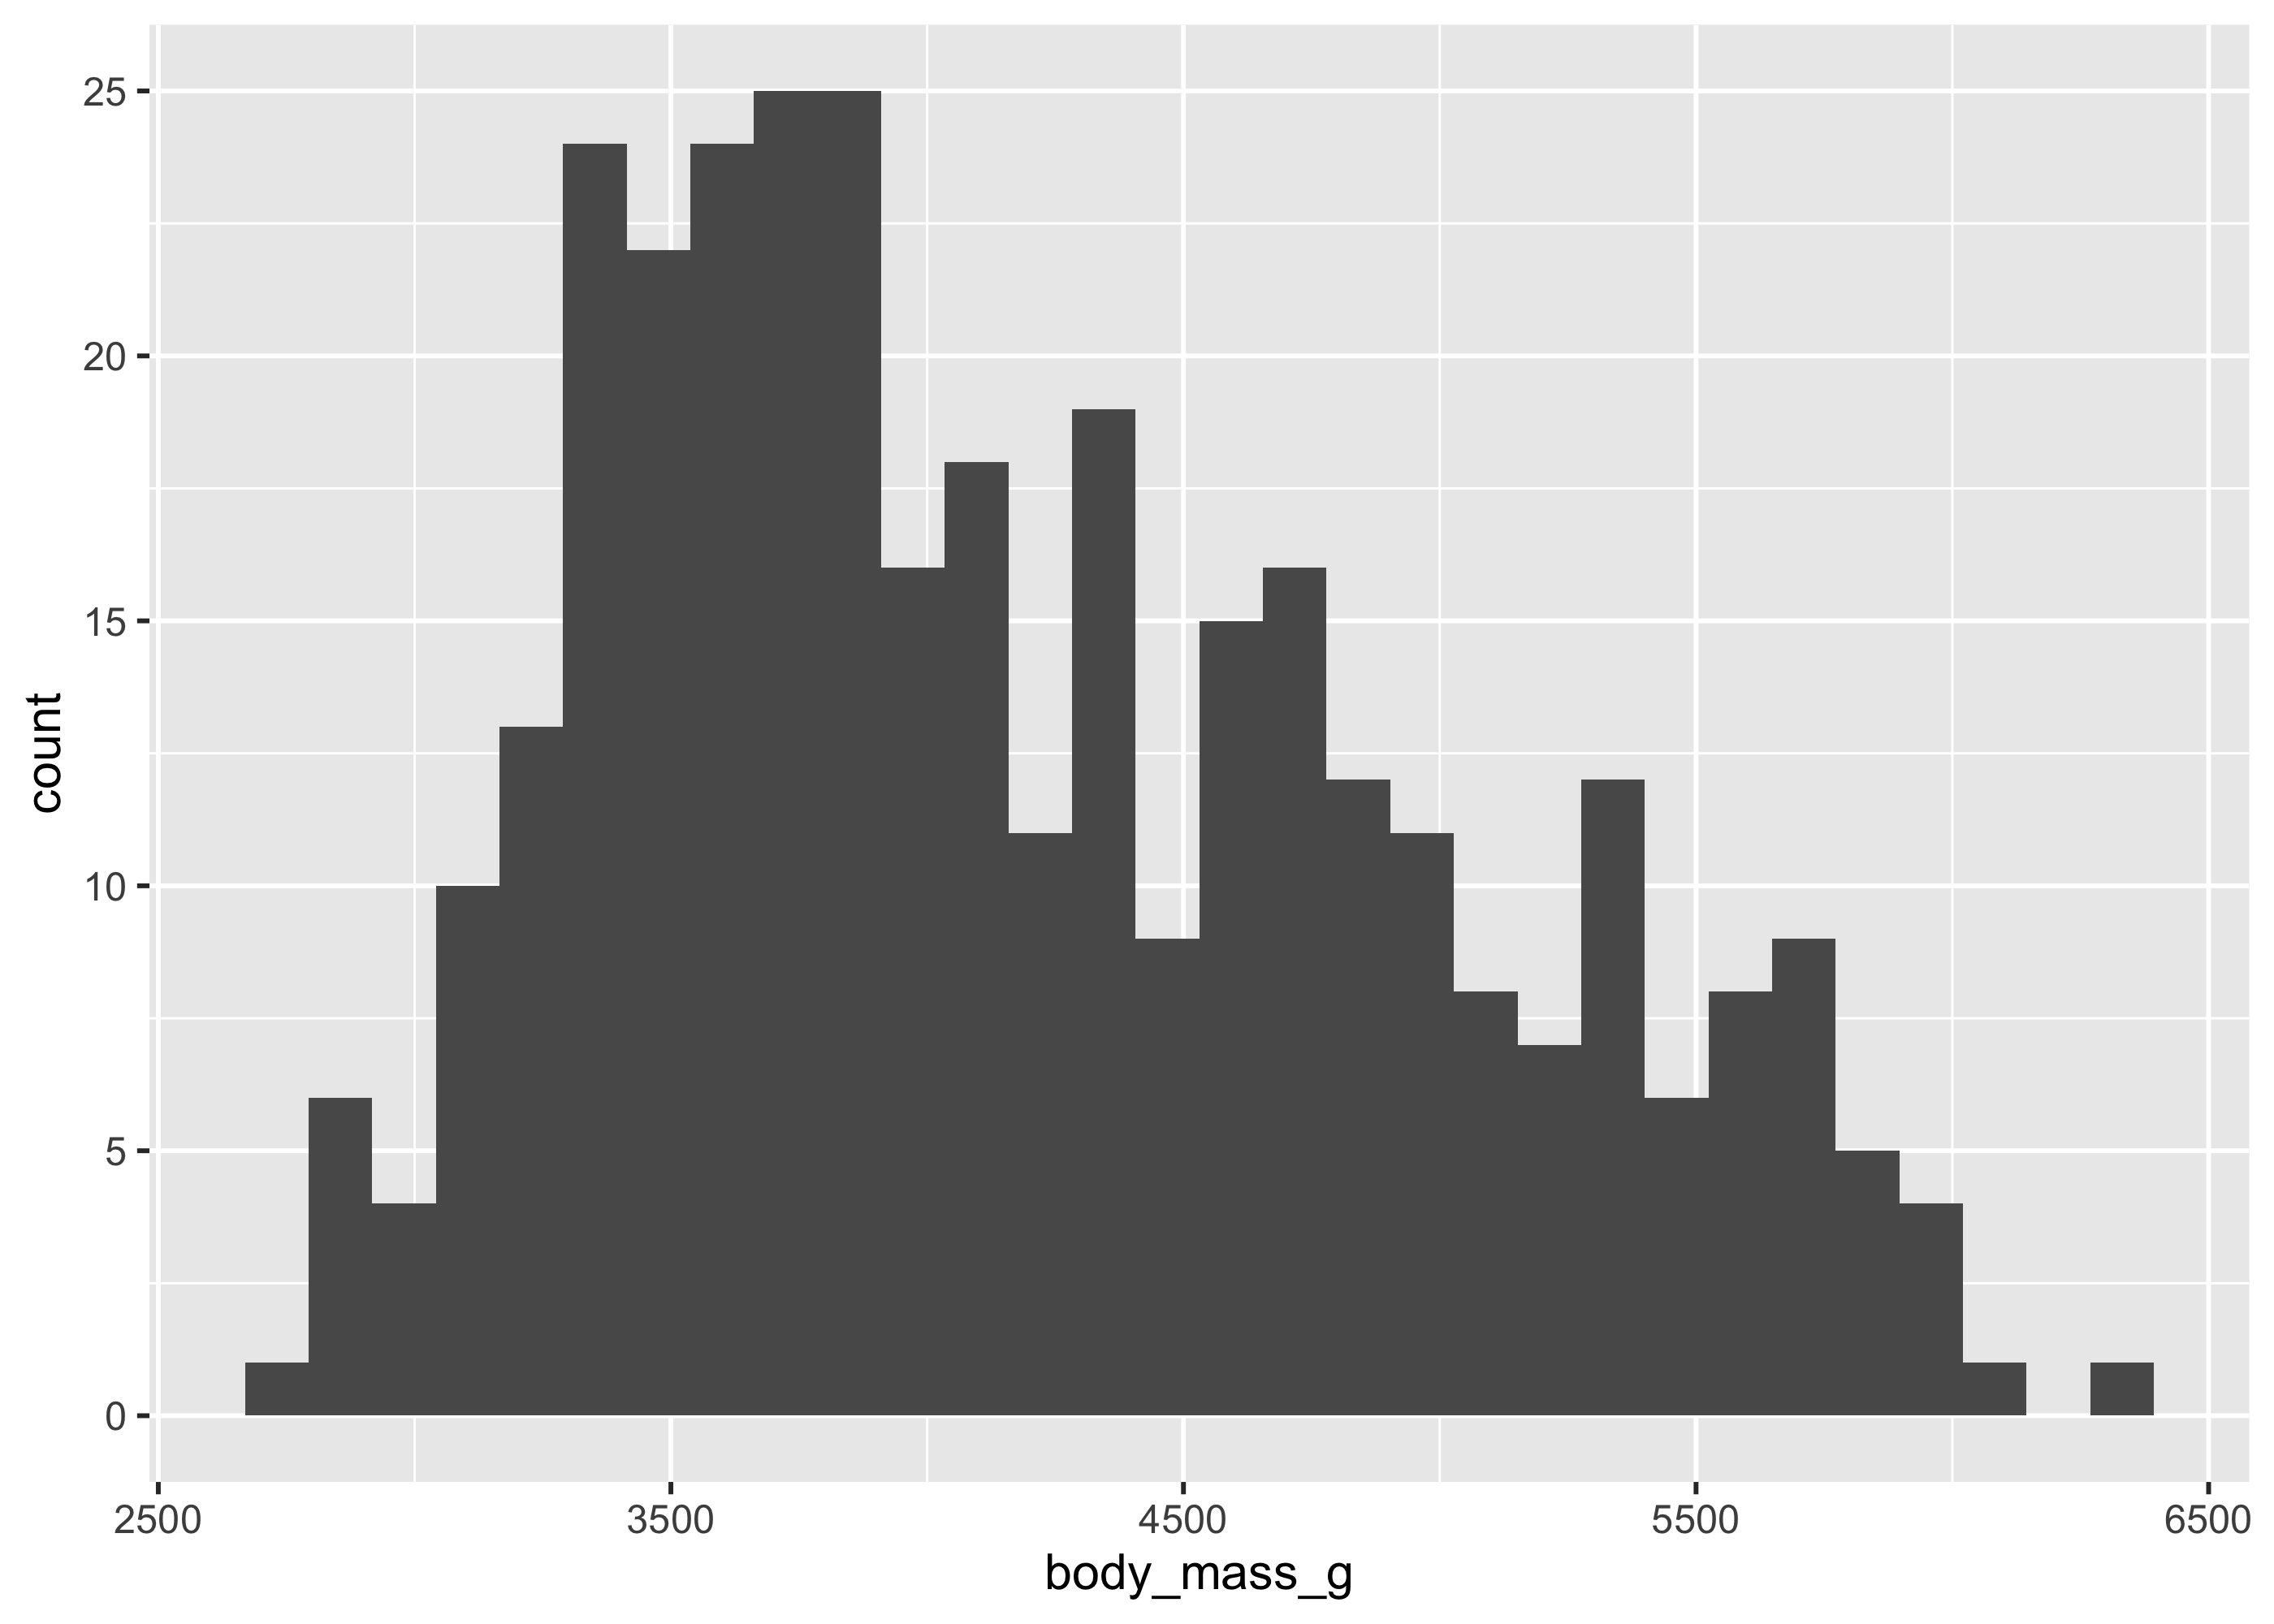
\includegraphics{visualizing-data-with-ggplot2_files/figure-pdf/unnamed-chunk-11-1.pdf}

}

\end{figure}

\hypertarget{coordinate-systems}{%
\subsection{Coordinate Systems}\label{coordinate-systems}}

Interpret the position aesthetics.

\begin{itemize}
\tightlist
\item
  \textbf{linear coordinate systems:} preserve the geometrical shapes

  \begin{itemize}
  \tightlist
  \item
    \texttt{coord\_cartesian()}
  \item
    \texttt{coord\_fixed()}
  \item
    \texttt{coord\_flip()}
  \end{itemize}
\item
  \textbf{non-linear coordinate systems:} likely change the geometrical
  shapes

  \begin{itemize}
  \tightlist
  \item
    \texttt{coord\_polar()}
  \item
    \texttt{coord\_map()} and \texttt{coord\_sf()}
  \item
    \texttt{coord\_trans()}
  \end{itemize}
\end{itemize}

The default coordinate system in ggplot is the cartesian coordinate
system. Generally, data viz folks hate pie charts because
\href{https://www.data-to-viz.com/caveat/pie.html}{they are not the best
way to visualize amounts and proportions}. There is not even
\texttt{geom\_piechart,} so to make one, you have to transform the
coordinate system like this.

\begin{Shaded}
\begin{Highlighting}[]
\NormalTok{penguins\_pie }\OtherTok{\textless{}{-}}\NormalTok{ penguins }\SpecialCharTok{|\textgreater{}}
\FunctionTok{group\_by}\NormalTok{(species) }\SpecialCharTok{|\textgreater{}}
\FunctionTok{summarise}\NormalTok{(}\AttributeTok{total =} \FunctionTok{n}\NormalTok{())}

\FunctionTok{ggplot}\NormalTok{(penguins\_pie,}
 \FunctionTok{aes}\NormalTok{(}\AttributeTok{x =}\NormalTok{ species,}
     \AttributeTok{y =}\NormalTok{ total,}
 \AttributeTok{fill =}\NormalTok{ species)) }\SpecialCharTok{+}
\FunctionTok{geom\_bar}\NormalTok{(}\AttributeTok{stat =} \StringTok{"identity"}\NormalTok{, }\AttributeTok{width =} \DecValTok{1}\NormalTok{ ) }\SpecialCharTok{+} 
\FunctionTok{coord\_polar}\NormalTok{(}\AttributeTok{start =} \DecValTok{0}\NormalTok{) }
\end{Highlighting}
\end{Shaded}

\begin{figure}[H]

{\centering 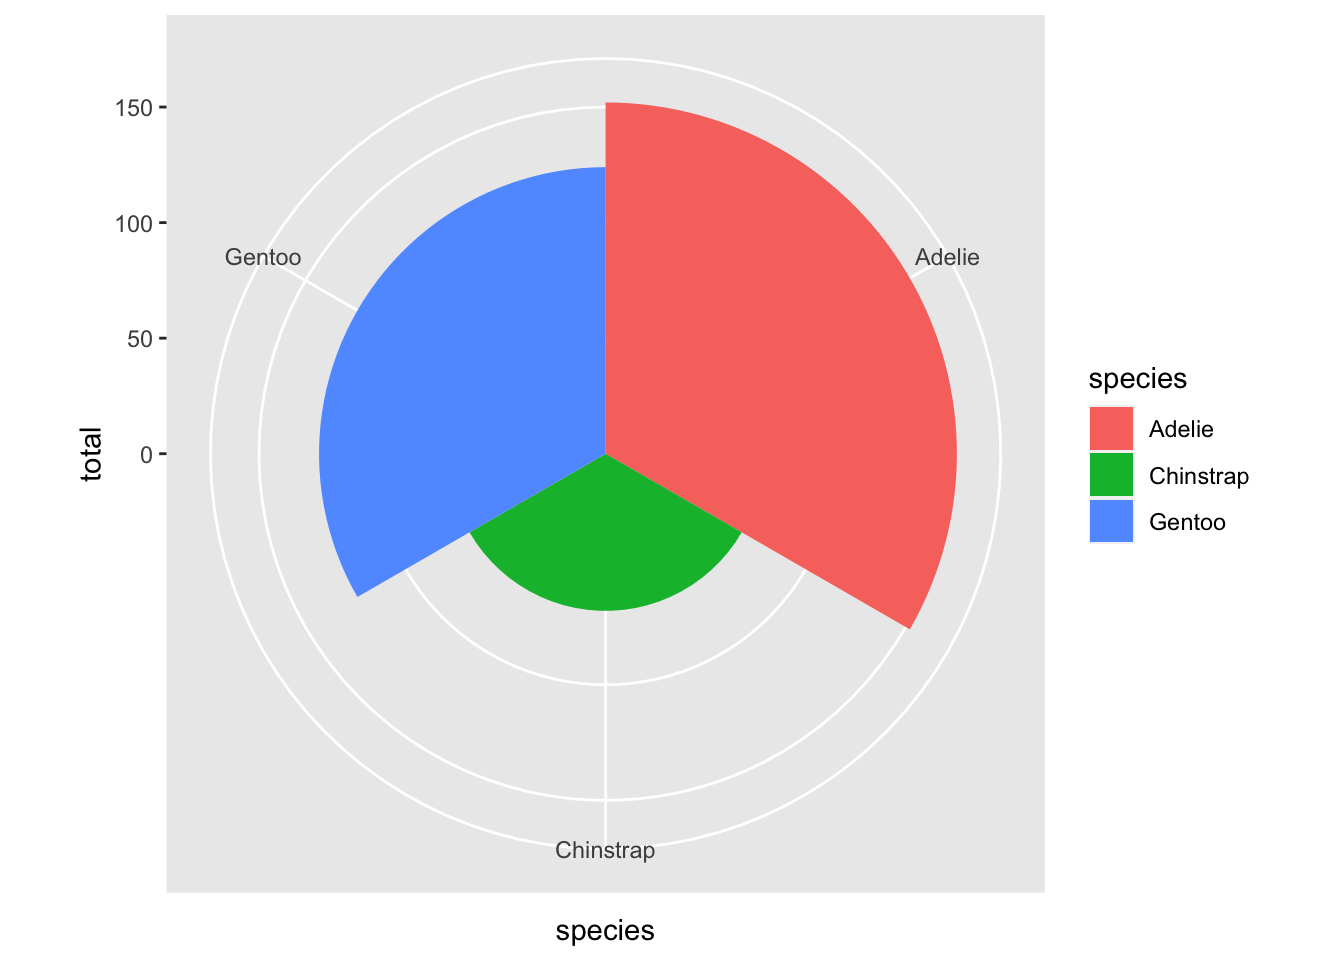
\includegraphics{visualizing-data-with-ggplot2_files/figure-pdf/unnamed-chunk-12-1.pdf}

}

\end{figure}

\hypertarget{facets}{%
\subsection{Facets}\label{facets}}

Facets are an excellent tool for data visualization. You are making a
plot for each value of a variable. Let's say we are interested in seeing
the subgroup differences of bill length and body mass but want to break
it out by sex. The most common ones you will see in the wild use
\texttt{facet\_wrap}

\begin{Shaded}
\begin{Highlighting}[]
\FunctionTok{ggplot}\NormalTok{(penguins,}
       \FunctionTok{aes}\NormalTok{(}\AttributeTok{x =}\NormalTok{ flipper\_length\_mm,}
           \AttributeTok{y =}\NormalTok{ body\_mass\_g,}
           \AttributeTok{color =}\NormalTok{ species,}
           \AttributeTok{shape =}\NormalTok{ species)) }\SpecialCharTok{+}
\FunctionTok{geom\_point}\NormalTok{() }\SpecialCharTok{+}
\FunctionTok{labs}\NormalTok{(}\AttributeTok{x =} \StringTok{"Flipper Length(mm)"}\NormalTok{, }\AttributeTok{y =} \StringTok{"Body Mass(g)"}\NormalTok{) }\SpecialCharTok{+}
\FunctionTok{facet\_wrap}\NormalTok{(}\FunctionTok{vars}\NormalTok{(sex))}
\end{Highlighting}
\end{Shaded}

\begin{figure}[H]

{\centering 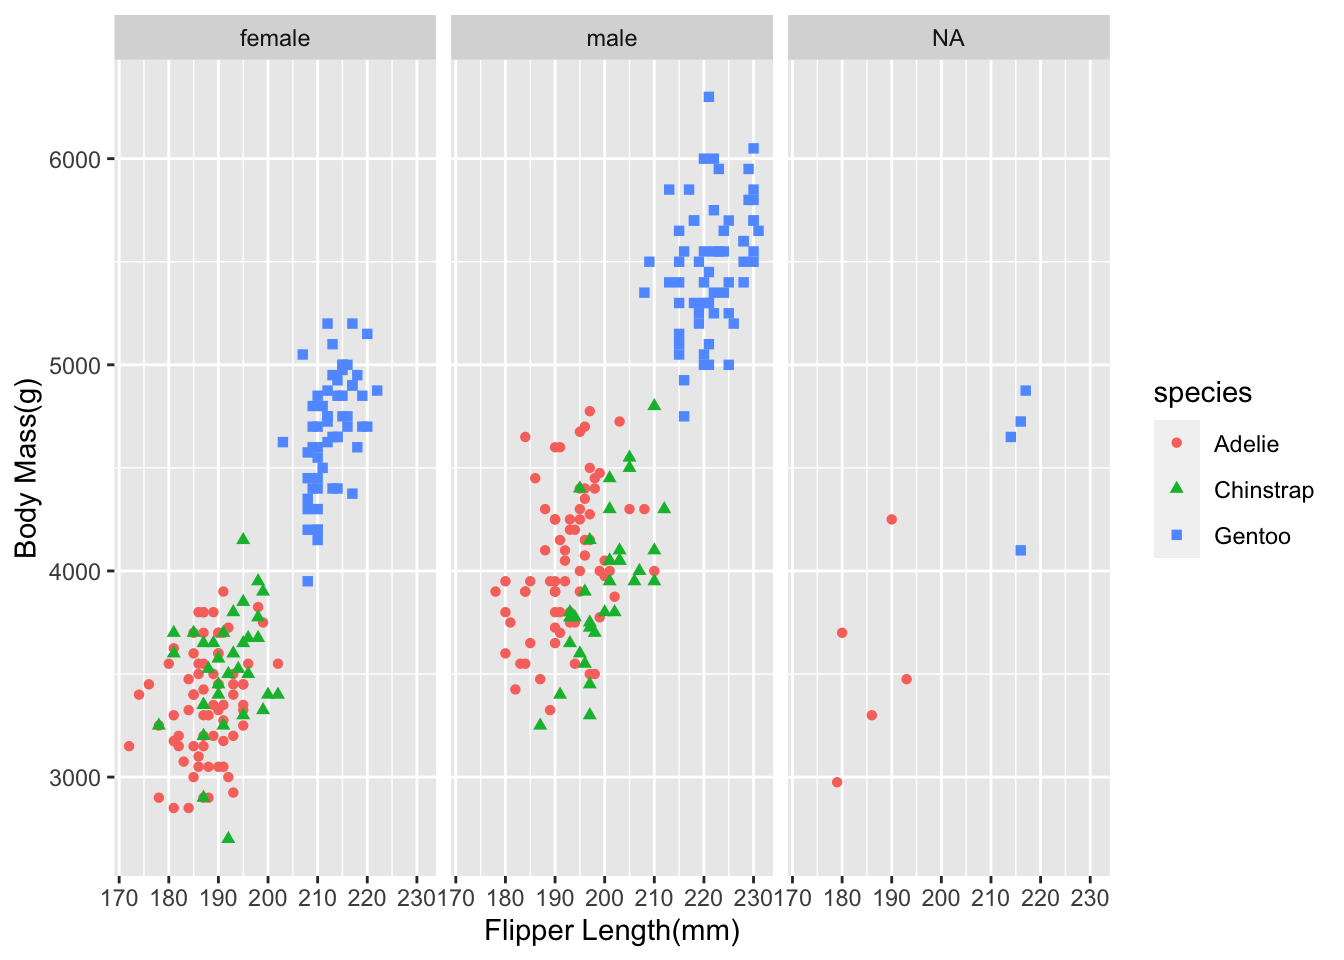
\includegraphics{visualizing-data-with-ggplot2_files/figure-pdf/unnamed-chunk-13-1.pdf}

}

\end{figure}

There is also something called \texttt{facet\_grid}, which forms a
matrix of panels defined by row and column faceting variables. It is
most useful when you have two discrete variables, and all combinations
of the variables exist in the data.

\begin{Shaded}
\begin{Highlighting}[]
\NormalTok{penguins\_no\_na }\OtherTok{\textless{}{-}}\NormalTok{ penguins }\SpecialCharTok{|\textgreater{}}
\FunctionTok{drop\_na}\NormalTok{()}

\FunctionTok{ggplot}\NormalTok{(penguins\_no\_na,}
      \FunctionTok{aes}\NormalTok{(}\AttributeTok{x =}\NormalTok{ flipper\_length\_mm,}
         \AttributeTok{y =}\NormalTok{ body\_mass\_g,}
         \AttributeTok{color =}\NormalTok{ species,}
         \AttributeTok{shape =}\NormalTok{ species)) }\SpecialCharTok{+}
\FunctionTok{geom\_point}\NormalTok{() }\SpecialCharTok{+}
\FunctionTok{labs}\NormalTok{(}\AttributeTok{x =} \StringTok{"Flipper Length(mm)"}\NormalTok{, }\AttributeTok{y =} \StringTok{"Body Mass(g)"}\NormalTok{) }\SpecialCharTok{+}
\FunctionTok{facet\_grid}\NormalTok{(}\FunctionTok{vars}\NormalTok{(sex), }\FunctionTok{vars}\NormalTok{(island))}
\end{Highlighting}
\end{Shaded}

\begin{figure}[H]

{\centering 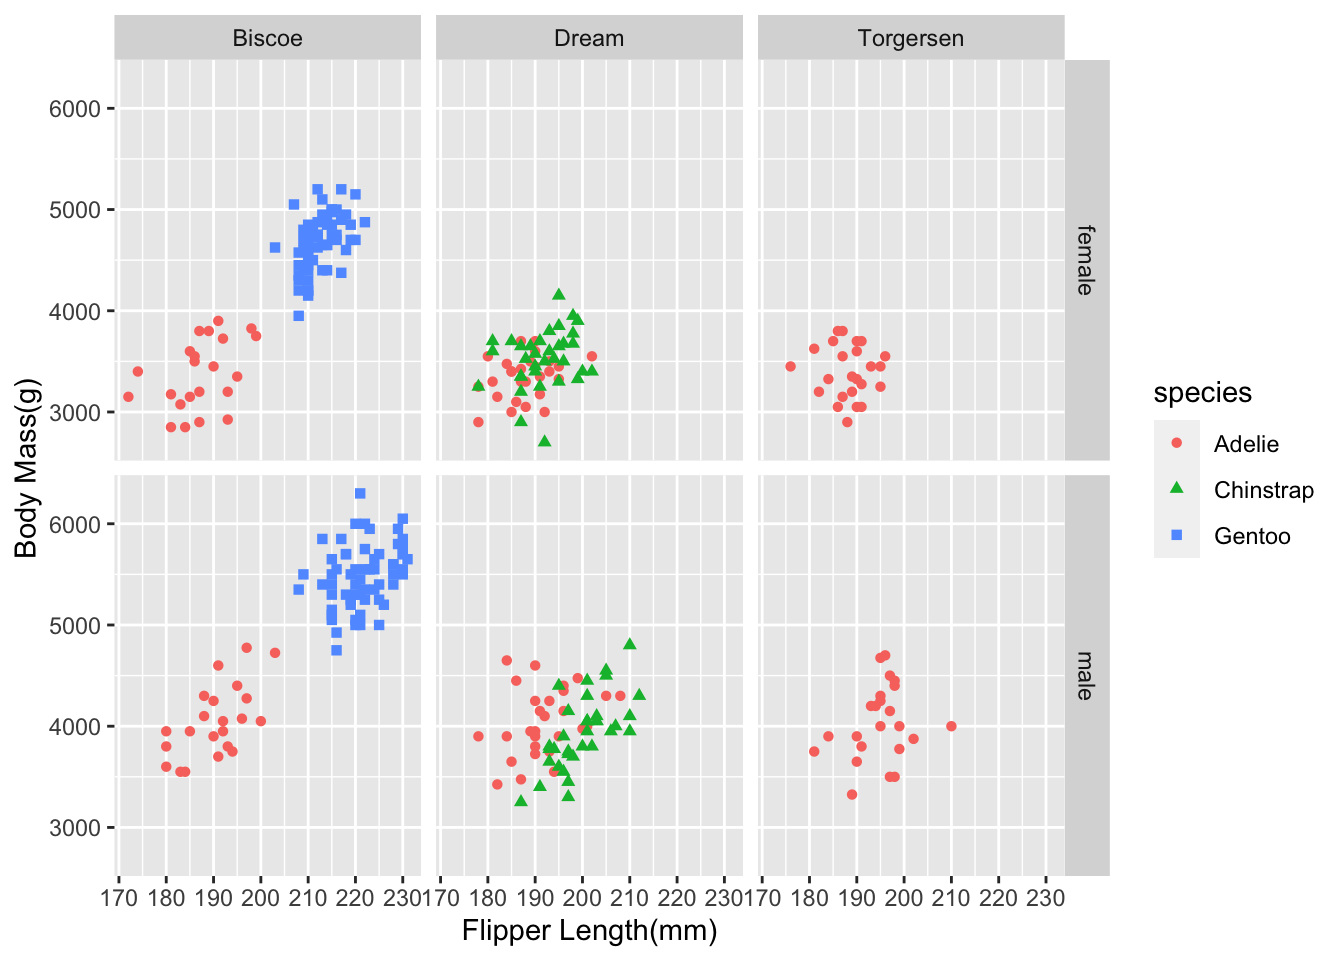
\includegraphics{visualizing-data-with-ggplot2_files/figure-pdf/unnamed-chunk-14-1.pdf}

}

\end{figure}

\hypertarget{themes-in-ggplot}{%
\subsection{Themes in ggplot}\label{themes-in-ggplot}}

Themes are just ways to customize everything that isn't data in your
plot. Themes make your graphs better looking and can make them stand
out. We have been working with the default theme, which I do not like,
but that is simply a matter of taste. Most people and organizations hate
it, so they immediately change the theme. The creator of ggplot will
defend it to his death which is a weird hill to die on.

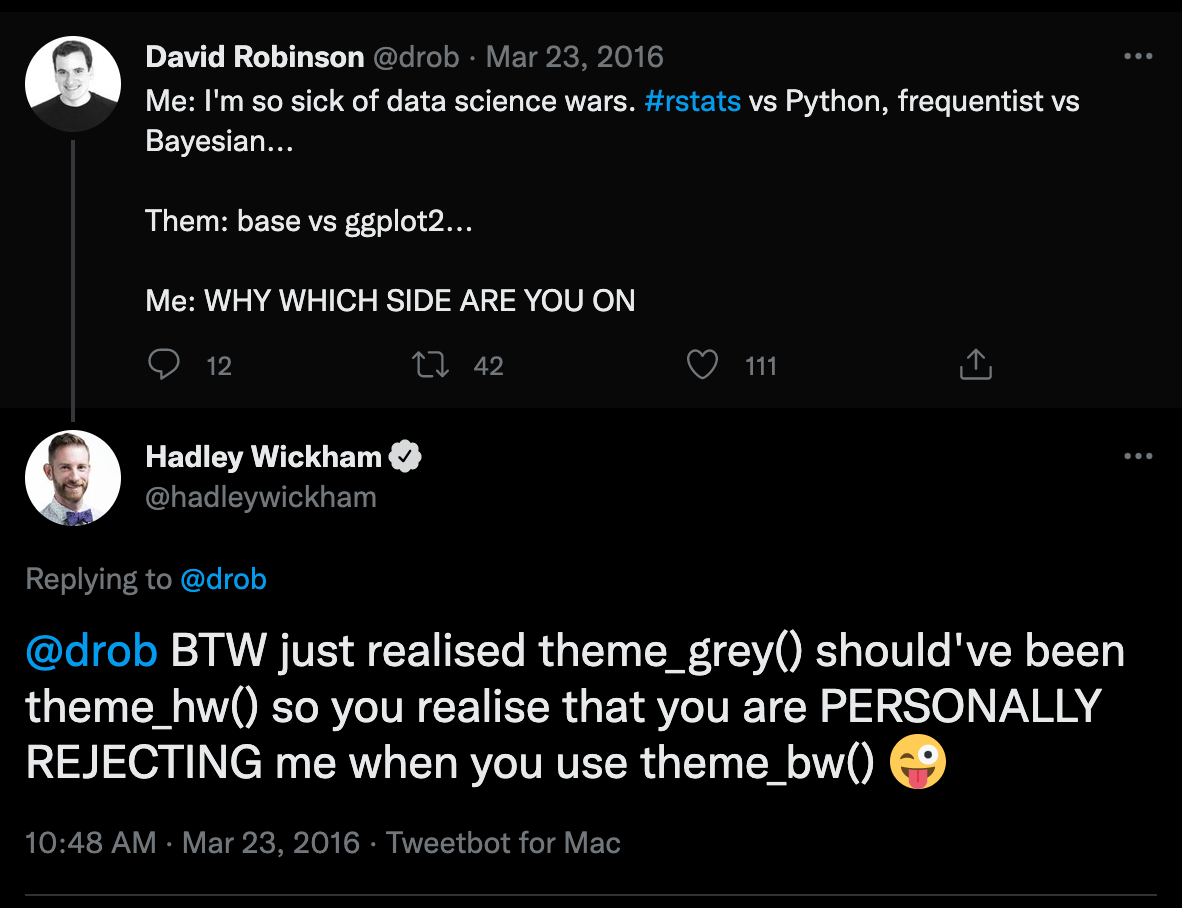
\includegraphics{figs/hadley_theme_grey.png}

To change the theme to something else, you add another layer once again.

\begin{Shaded}
\begin{Highlighting}[]
\FunctionTok{ggplot}\NormalTok{(penguins\_no\_na,}
      \FunctionTok{aes}\NormalTok{(}\AttributeTok{x =}\NormalTok{ flipper\_length\_mm,}
          \AttributeTok{y =}\NormalTok{ body\_mass\_g,}
         \AttributeTok{color =}\NormalTok{ species,}
         \AttributeTok{shape =}\NormalTok{ species)) }\SpecialCharTok{+}
\FunctionTok{geom\_point}\NormalTok{() }\SpecialCharTok{+}
\FunctionTok{labs}\NormalTok{(}\AttributeTok{x =} \StringTok{"Flipper Length(mm)"}\NormalTok{, }\AttributeTok{y =} \StringTok{"Body Mass(g)"}\NormalTok{) }\SpecialCharTok{+}
\FunctionTok{scale\_color\_met\_d}\NormalTok{(}\AttributeTok{name =} \StringTok{"Demuth"}\NormalTok{) }\SpecialCharTok{+}
\FunctionTok{theme\_bw}\NormalTok{()}
\end{Highlighting}
\end{Shaded}

\begin{figure}[H]

{\centering 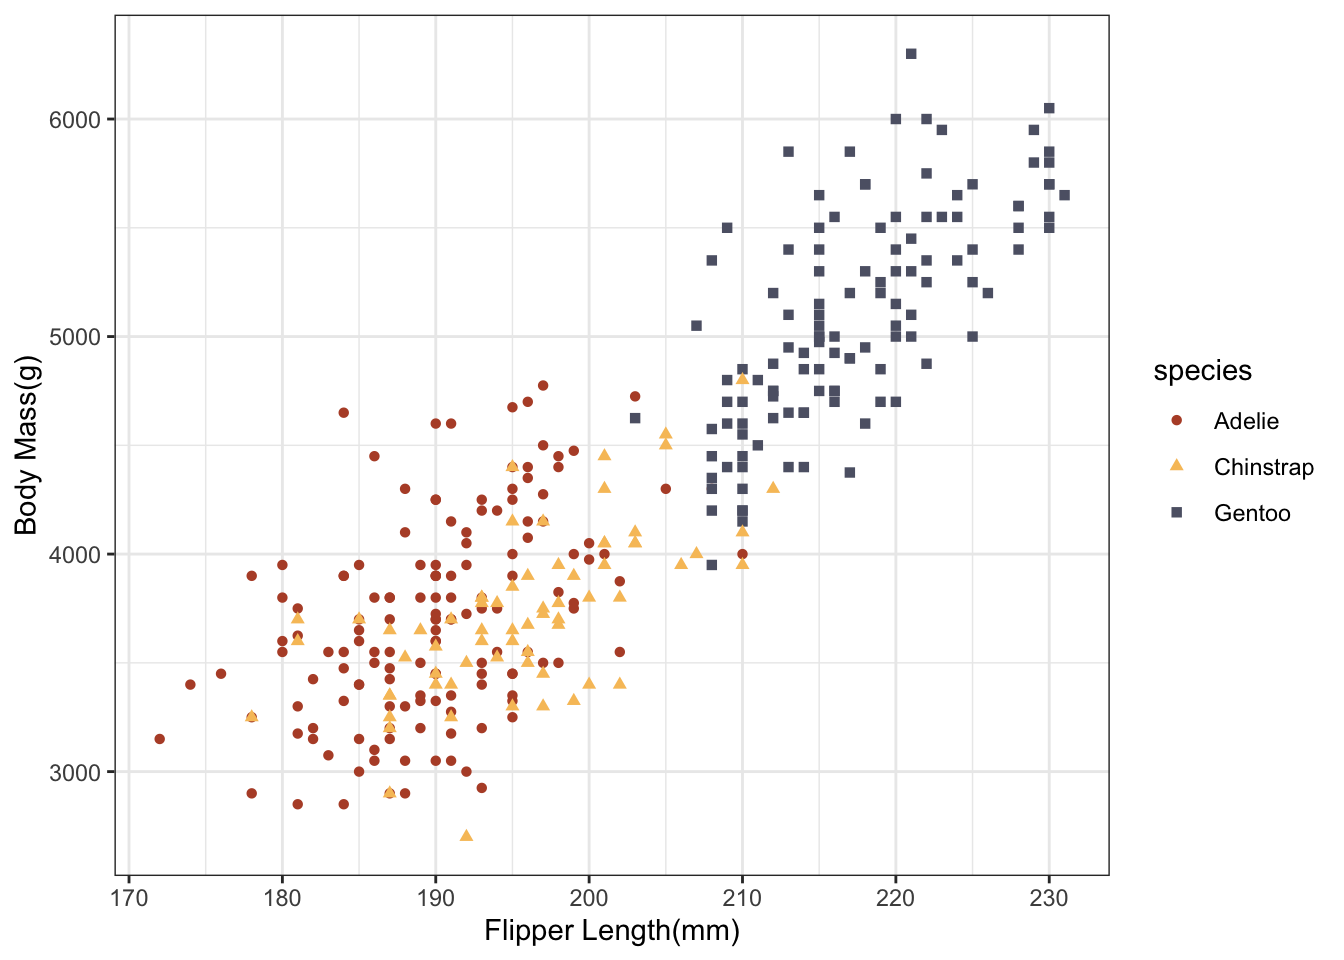
\includegraphics{visualizing-data-with-ggplot2_files/figure-pdf/unnamed-chunk-15-1.pdf}

}

\end{figure}

There are lots of user-written themes that look good. You can search the
internet to find them. \texttt{theme\_bw} is a function that changes a
whole host of things in the theme layer. I have my own bespoke theme
that I use in class all the time that looks something like this.

\begin{Shaded}
\begin{Highlighting}[]
\NormalTok{theme\_allen }\OtherTok{=} \ControlFlowTok{function}\NormalTok{()\{}
  \FunctionTok{theme\_minimal}\NormalTok{(}\AttributeTok{base\_family =} \StringTok{"Roboto Condensed"}\NormalTok{, }
                \AttributeTok{base\_size =} \DecValTok{14}\NormalTok{)  }\SpecialCharTok{+}
    \FunctionTok{theme}\NormalTok{(}\AttributeTok{axis.ticks =} \FunctionTok{element\_line}\NormalTok{(}\AttributeTok{colour=}\StringTok{\textquotesingle{}black\textquotesingle{}}\NormalTok{),}
          \AttributeTok{plot.background =} \FunctionTok{element\_blank}\NormalTok{(),}
          \AttributeTok{panel.grid.minor =} \FunctionTok{element\_blank}\NormalTok{(),}
          \AttributeTok{panel.grid.major =} \FunctionTok{element\_line}\NormalTok{(}\AttributeTok{linetype =} \StringTok{"dotted"}\NormalTok{, }
                                          \AttributeTok{color =} \StringTok{"\#BBBBBB"}\NormalTok{),}
          \AttributeTok{legend.background =} \FunctionTok{element\_rect}\NormalTok{(}\AttributeTok{color =} \StringTok{"white"}\NormalTok{),}
          \AttributeTok{legend.title =} \FunctionTok{element\_text}\NormalTok{(}\AttributeTok{face =} \StringTok{"bold"}\NormalTok{),}
          \AttributeTok{axis.title.x =} \FunctionTok{element\_text}\NormalTok{(}\AttributeTok{margin =} \FunctionTok{margin}\NormalTok{(}\AttributeTok{t =} \DecValTok{10}\NormalTok{), }\AttributeTok{hjust =} \DecValTok{0}\NormalTok{),}
          \AttributeTok{axis.title.y =} \FunctionTok{element\_text}\NormalTok{(}\AttributeTok{margin =} \FunctionTok{margin}\NormalTok{(}\AttributeTok{r =} \DecValTok{10}\NormalTok{), }\AttributeTok{hjust =} \DecValTok{1}\NormalTok{),}
          \AttributeTok{strip.background =} \FunctionTok{element\_rect}\NormalTok{(}\AttributeTok{fill =} \StringTok{"white"}\NormalTok{, }\AttributeTok{color =} \ConstantTok{NA}\NormalTok{),}
          \AttributeTok{panel.border =} \FunctionTok{element\_rect}\NormalTok{(}\AttributeTok{color =} \StringTok{"grey90"}\NormalTok{, }\AttributeTok{fill =} \ConstantTok{NA}\NormalTok{))}
  
\NormalTok{\}}
\end{Highlighting}
\end{Shaded}

\marginnote{\begin{footnotesize}

The theme I use in class and in my work is just various tweaks to
\href{https://github.com/kylebutts/templates/blob/master/ggplot_theme/theme_kyle.R}{Kyle
Butt's ggplot theme}

\end{footnotesize}}

Covering all possible ways to modify a theme would require much more
time. There are something like 94 different arguments you can modify in
theme to change virtually anything you can think of in your figure. I
will frequently use the theme argument in my work to just make minor
tweaks like changing the legend position.

\begin{Shaded}
\begin{Highlighting}[]
 \FunctionTok{ggplot}\NormalTok{(penguins\_no\_na,}
       \FunctionTok{aes}\NormalTok{(}\AttributeTok{x =}\NormalTok{ flipper\_length\_mm,}
           \AttributeTok{y =}\NormalTok{ body\_mass\_g,}
           \AttributeTok{color =}\NormalTok{ species,}
           \AttributeTok{shape =}\NormalTok{ species)) }\SpecialCharTok{+}
\FunctionTok{geom\_point}\NormalTok{() }\SpecialCharTok{+}
\FunctionTok{labs}\NormalTok{(}\AttributeTok{x =} \StringTok{"Flipper Length(mm)"}\NormalTok{, }\AttributeTok{y =} \StringTok{"Body Mass(g)"}\NormalTok{) }\SpecialCharTok{+}
\FunctionTok{scale\_color\_met\_d}\NormalTok{(}\AttributeTok{name =} \StringTok{"Demuth"}\NormalTok{) }\SpecialCharTok{+}
\FunctionTok{theme\_bw}\NormalTok{() }\SpecialCharTok{+} 
\FunctionTok{theme}\NormalTok{(}\AttributeTok{legend.position =} \StringTok{"bottom"}\NormalTok{)}
\end{Highlighting}
\end{Shaded}

\begin{figure}[H]

{\centering 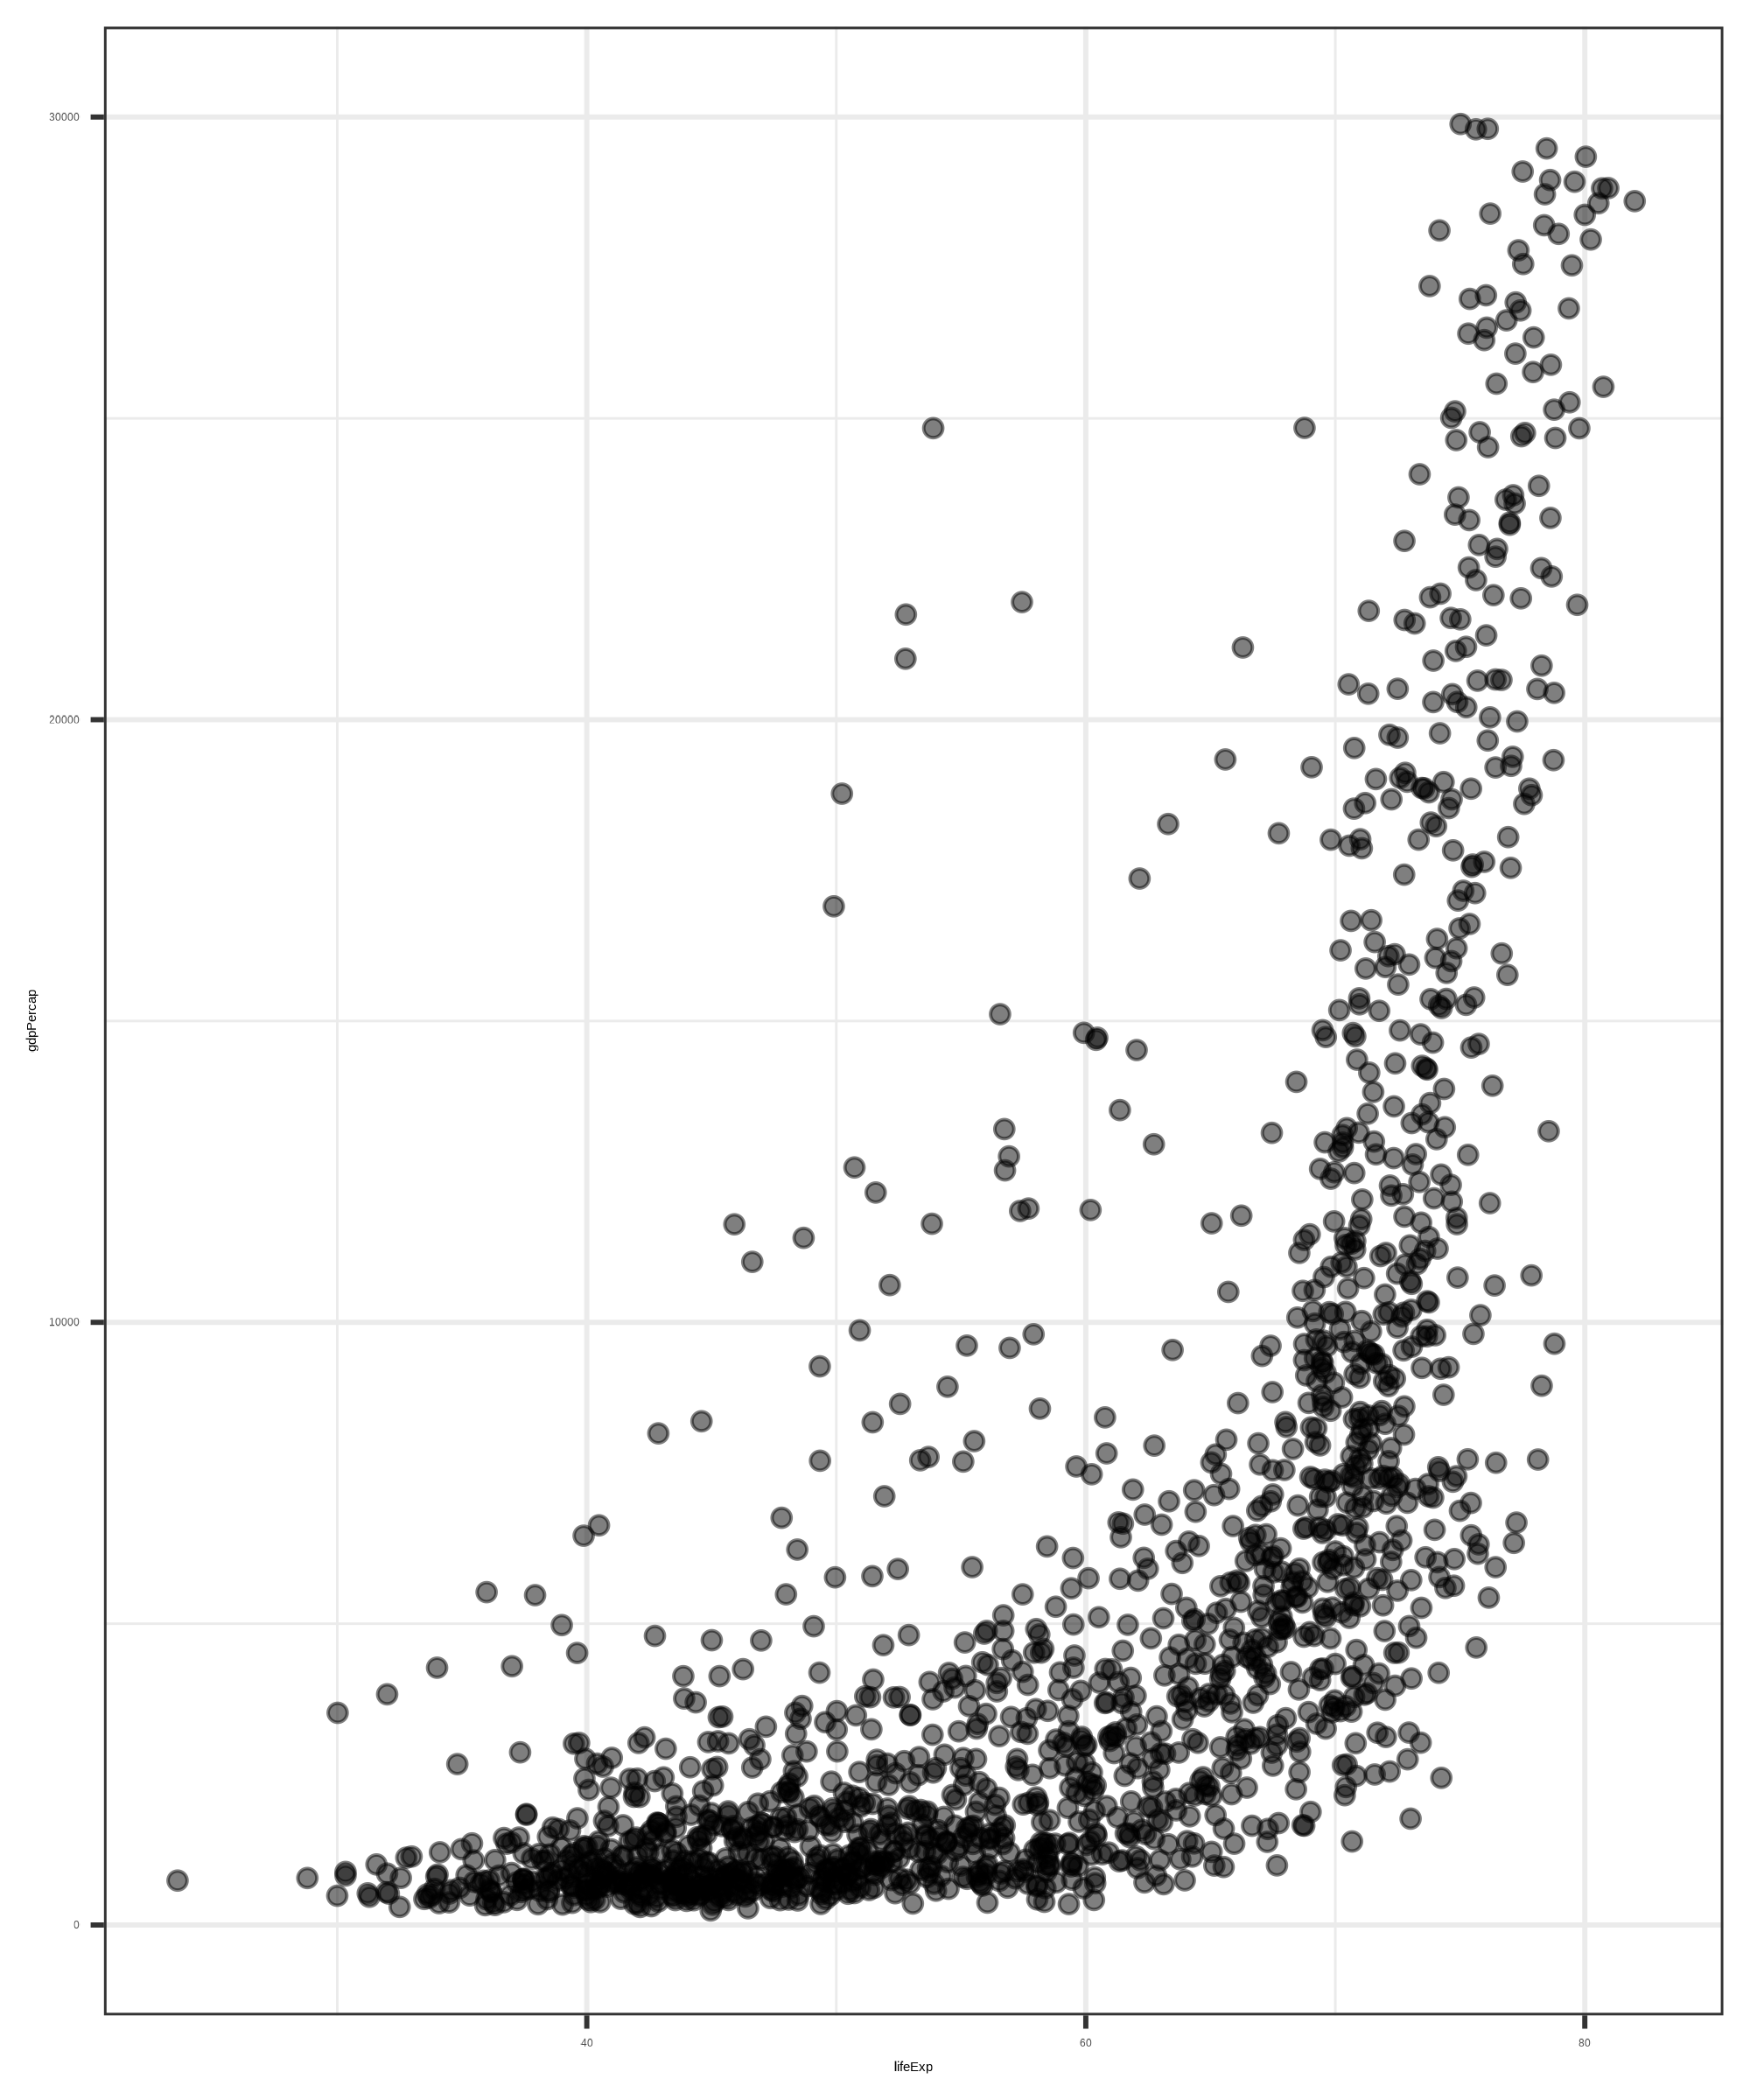
\includegraphics{visualizing-data-with-ggplot2_files/figure-pdf/unnamed-chunk-17-1.pdf}

}

\end{figure}

\hypertarget{saving-your-work}{%
\subsection{Saving your work}\label{saving-your-work}}

Finally, the last thing is I will show you in ggplot is how to save your
plot.

\begin{Shaded}
\begin{Highlighting}[]
\NormalTok{your\_plot\_here }\OtherTok{=} \FunctionTok{ggplot}\NormalTok{(data, }\FunctionTok{aes}\NormalTok{(}\AttributeTok{x =}\NormalTok{ blah, }\AttributeTok{y =}\NormalTok{ blah))}
\end{Highlighting}
\end{Shaded}

\begin{Shaded}
\begin{Highlighting}[]
\FunctionTok{ggsave}\NormalTok{(}\StringTok{"name{-}of{-}your{-}file.pdf"}\NormalTok{,your\_plot\_here) }
\end{Highlighting}
\end{Shaded}

\begin{Shaded}
\begin{Highlighting}[]
\FunctionTok{ggsave}\NormalTok{(}\StringTok{"name{-}of{-}your{-}file.pngs"}\NormalTok{,your\_plot\_here)}
\end{Highlighting}
\end{Shaded}

\part{Beyond the Basics of The Tidyverse}



\end{document}
